One view to take on this is to give enough material such that the rest of the thesis is understandable, at least in concept from here. I am thinking to write in such a way that the questions answered by the papers become obvious ones to ask.

\subsection{Einstein summation convention}

Typical notation in the study of manifolds is the \emphmarginnote{Einstein summation convention}. In many places we will see sums of the form \(\sum_i x^i E_i\). It is notationally helpful therefore to have a shorthand for this. We write \[E(x) = x^i E_i, \quad \text{ as an abbreviation of } E(x) = \sum_{i=1}^n x^i E_i\]. In general
\1 Indices that appear twice it is assumed we sum over all values of these indices.
\2 Indices that appear once index the output of the expression.
\3 Basis vectors are always written with subscripts.
\4 Basis coefficients are written with superscripts. 
\0
Point 3\&4 help us keen notation sane. Typically, under this convention we would expect to see an index appear once as an upper index and once as a lower. Violation of this rule might indicate something is awry. Some illustrative examples can be given by:
\begin{itemize}
    \item A vector in a basis \(\cbr{e_i}\) with coefficients \(\cbr{v^i}\) is written as \(v = v^i e_i\).
    \item A matrix-vector multiplication, \(\v{y} = \m{M}\v{x}\), \(y_j = \sum_{i=i}^n M_{ji} x_i \)would be written as  \(y^j = M^{ji} x^i \).
    \item A matix-matrix multiplication, \(\m{C} = \m{A}\m{B}\), \(\m{C}_{ik} = \sum_{j=1}^n \m{A}_{ij}\m{B}_{jk}\), would be written as \(C^{ik} = A^{ij} B^{jk}\).
    \item The inner product \(\v{u} \cdot \v{v} = u^j v^j\).
    \item 
\end{itemize}
\todo{Improve this. SOrt out the different intepretations of the convention.}

\section{Set theory}

The construction of all math lies upon set theory. Starting from a set of simple axioms, we can build all of the beauty of modern mathematics. Caution though, these are not the only axioms we could choose, and indeed there is great debate over one in particular, the axiom of choice. There exist a number of set theories, but the most common is Zermelo–Fraenkel, with or without the axiom of choice (ZF or ZFC). We can also start mathematics with type-theory - but this can be shown to be identical to choices of set theory. The following is an informal introduction.

A \emphmarginnote{set} is a collection of mathematical objects, typically denoted with curly brackets \(\cbr{}\). For example if there exist such objects as \(\cbr{}\) 

\section{Basic Algebra}

From sets we can begin to construct more interesting mathematical objects by combining sets with operations on sets. These operation take elements of sets and map them to elements of sets. An operation, or function \(f\), that maps objects from set \(X\) to set \(Y\) is typically denoted \(f: X \to Y\). 

\subsection{Vector spaces and linear algebra}

A \emphmarginnote{vector space} over a given field \(F\) (a set with the typical notions of addition, \(+_F\) and multiplication \(\times_F\), and their inverses) is a set \(V\) equipped with two operation, \(+: V \times V\to V\), \emphmarginnote{vector addition}, under which the vector space is an abelian group, and \(\cdot:  F \times V \to V\), \emphmarginnote{scalar multiplication}, such that \(a \cdot( b \cdot v) = (a \times_f b)\cdot v\) and \(1\cdot v = v\) for \(a, b \in F, v\in V\), and \(1\) the identity element of the field multiplication. In addition the field and vector operations must be suitably distributive \[(a +_F b) \cdot v = a \cdot v + b \cdot v \quad\quad a\cdot (v + w) = a\cdot v + a \cdot w\quad\quad a,b \in F, \; w,v\in V \]. A \emphmarginnote{topological vector space} is a vector space over a topological field, equipped with a topology so that vector addition and scalar multiplication are continuous. Most commonly we deal with vector spaces over the \emph{real numbers} \(\R\), but sometimes also over the \emph{complex numbers} \(\C\). From now on we will only discuss real vector spaces.

A subset of a vector space that is closed under the vector operation is called a \emphmarginnote{linear subspace}, distinct from a topological subspace. If we have a finite set of vectors \(S = \cbr{v_1, ..., v_n}, v_i \in V\), a \emphmarginnote{linear combination} of them is denoted by \(\sum_{i=1}^n a_i v_i\) with \(a_i \in \R\). The \emphmarginnote{span} of a set of vectors, denoted \(\Span(S)\) is the set of all linear combinations of the vectors, and is a linear subspace. If \(V = \Span(S)\) then \(S\) \emph{spans} \(V\). A set \(S\) is said to be \emphmarginnote{linearly dependant} is there exist \(a_i\in \R\) such that the linear combination is \(0\in V\). Otherwise they are \emphmarginnote{linearly independent}.

A \emphmarginnote{basis} for \(V\) is a linearly independent subset \(S \subseteq V\) such that \(\Span(S) = V\). Every \(v\in V\) has a \emph{unique} expression as a linear combination of the basis.  The choice of basis is non-unique, although often there is a sensible choice. All bases of a vector space are of the same cardinality, called the dimension of the space, \(\dim V\).If the basis is finite of size \(n\), the space is said to be finite-dimension or \(n-\)dimension. If it is infinite, infinite-dimension. If we can ascribe an order to a basis (if it is finite or countable) the we call it an \emphmarginnote{ordered basis}, and we can identify the elements \(v\in V\) of the vector space with the ordered set of field coefficients \(\del{a_i1, ...}\) such that \(\sum_i a^i v_i  = v\). This is called the \emphmarginnote{basis representation}. All bases of the same vector space are of the same dimension.

\(n\)\emph{-dimension Euclidean space}\marginnote{\(n\)-dimension Euclidean space}, \(\R^n\) is the prototypical example of a finite-dimension real vector space with vector and scalar multiplication defined by\[(x_1, ..., x_n) + (Y-1, ..., y_n) &= (x_1 + y_1, ..., x_n + y_n) \\ a(x_1, ..., x_n) &= (ax_1, ..., ax_n)\], with standard basis \((e_1, ..., e_n)\), \(e_i = (0,..., 1, ..., 0)\) with the \(1\) in the i'th position. 

\textcolor{red}{some inf dim one?}

A \emphmarginnote{linear map} between vector spaces \(V\) and \(W\) are maps \(T: V \to W\) such that they preserve the structure of vector addition and scalar multiplication. I.e. \(T(av + bw) = aT(v) + bT(w)\). A map \(T: V \to \R\) is called a \emphmarginnote{linear functional}. The \emphmarginnote{image} of \(T\), \(\im T\) is the set \(\im T = \cbrcolon{w = T(v)}{v \in V}\). The \emphmarginnote{kernel} or \emphmarginnote{null space} of \(T\), \(\ker T\) is the preimage of \(0\) under \(T\), \(\ker T = \cbrcolon{v}{T(v) = 0, v\in V}\).

If \(V, W\) are vector spaces, a bijective linear map \(T: V \to W\) is called a \emphmarginnote{vector isomorphism}, \(T\) has an inverse, and \(V, W\) are said to be (vector) isomorphic, \(V \isomvec W\).

\subsection{Tensors}
\label{sec:tensors}
\subsubsection{Covectors}

For any vector space \(V\), we can define a \emphmarginnote{covector} as a linear map \(\omega: V \to \R\). We call the space of covectors the \emphmarginnote{dual space} of \(V\), denoted \(V^*\).  For a finite dimension vector space, if we have a basis on \(V\), \(e_1, ..., e_n\), then we can define the \emphmarginnote{standard dual basis} \(\epsilon^1, ..., \epsilon^n\) on \(V^*\) by \(\epsilon^i(e_j) = \delta^i_j\), showing it is also \(n\)-dimension. Note the use of upper indices, inline with Einstein summation notation. We write basis vectors of the dual space with upper indices so that they appear once upper and once lower when computing the interaction of a vector and a covector. \[\omega(v) = (\omega_i\epsilon^i)(v^je_j) = \omega_iv^j \epsilon^i(e_j) = \omega_iv^j \delta^j_i = \omega_i v^i\] 

For any linear map \(A: V\to W\), we can define its \emphmarginnote{dual map}, \emph{transpose}, or \emphmarginnote{adjoint} \(A^*: W^* \to V^*\) as the map \[(A^*\omega)(v) = \omega(Av), \quad \omega \in W^*, v \in v\]. This adjoint distributes over composition, but reverse terms, \((A\circ B)^* = B^* \circ A^*\), and preserves the identity, \((\id_V)^* = \id_{V^*}\). 

The \emphmarginnote{double dual} of \(V\), \(V^{**} = (V^*)^*\), the dual of the dual, for finite dimension vector spaces is isomorphic to the original space \(V\). There is a natural map \(\xi: V \to V^{**}\) as \[\xi(v)(\omega) = \omega(v) \quad, \omega \in V^*,  v \in V\]. Because we can unambiguously identify \(V\) with \(V^{**}\) for finite dimension vector spaces, we typically only talk about \(V\) and its dual \(V^*\). Sometimes one may see the inner product between a vector and a covector written as \(\innerprod{\omega}{v}\) or \(\innerprod{v}{\omega}\). The second denotes the action of \(\xi(v)\) on \(\omega\), but the result of both are identical.

\subsubsection{Higher order tensors}
Covectors defined linear maps over vector spaces. Tensors allow us to define \emphmarginnote{multilinear maps}. For vector spaces \(V_1, ..., V_k, W\), a multilinear map is a map \(f: V_1 \x ... \x V_k \to W\) if for any \(i\), \[f(v_1, ..., a v_i + b v'_i, ..., v_k) = a f(v_1, ..., v_i, ..., v_k) + b f(v_1, ..., v'_i, ..., v_k)\]. Tensors are multilinear maps over copies of the same vectors space and its dual. We can define multilinear maps

\begin{tabular}{lcc}
    \scshape Map & \scshape Notation & \scshape "Archaic" name \\ 
    \(f: \underbracket{V\x ... \x V}_{k \text{ copies}} \to \R \) & \(T^k(V^*) = T^{(0,k)}(V)\)& covariant \(k\)-tensor on \(V\)\\
    \(f: \underbracket{V^* \x ... \x V^*}_{k \text{ copies}} \to \R \) & \(T^k(V) = T^{(k,0)}(V)\)& contravariant \(k\)-tensor on \(V\)\\
    \(f: \underbracket{V^*\x ... \x V^*}_{k \text{ copies}}\x \underbracket{V \x ... \x V}_{l \text{ copies}} \to \R \) & \(T^{(k,l)}(V)\) & mixed \((k,l)\)-tensor on \(V\)\\
\end{tabular}

The "archaic" name refers to how the basis coefficients transform with the basis vectors. \emph{Covariant} tensor basis coefficients transform \emph{with} them, and \emph{contravariant} \emph{opposite} to them. In the modern setting where we typically work basis-free these make less sense. By convention, and for sensible reasons, the a tensor in \(T^{(0,0)}\) is just a scalar. 

The \emphmarginnote{tensor product} is an operation \(\otimes: T^{(k,l)}(V) \x T^{(p,q)}(V)\to T^{(k+p, l+q)}(V)\). It is defined by its evaluation \[\del{F\otimes G}(\omega^1, ..., \omega^k, \omega^{k+1}, ..., \omega^{k+p}, v_1, ..., v_l, v_{l+1}, ..., v_{l+q})\\ = F(\omega^1, ..., \omega^k, v_1, ..., v_l) G(\omega^{k+1}, ..., \omega^{k+p}, v_{l+1}, ..., v_{l+q})\]. This is an associative but \emph{not} a commutative operation. We can build a \emphmarginnote{basis on a tensor space} then out of the basis on \(V\) and \(V^*\), giving basis elements of the form \[e_{i_1}\otimes ...\otimes e_{i_k}\otimes \epsilon^{j_1},  \otimes ...\otimes \epsilon^{j_l}, \quad\quad i_{a}\in [1,..., k], \; j_b \in [1,..., l]\] with the obvious action on basis vectors \[e_{i_1}\otimes ...\otimes e_{i_k}\otimes \epsilon^{j_1},  \otimes ...\otimes \epsilon^{j_l}\del{\epsilon^{s_1}, ..., \epsilon^{s_k}, e_{t_1}, ..., e_{t_l}} = \delta^{s_1}_{i_1} ... \delta^{s_k}_{i_k} \delta^{j_1}_{t_1} ... \delta^{j_l}_{t_l} \]. This makes a \(T^{(k,l)}(V)\) of a \(n\)-dimension vector space a \(n^{k+l}\)-dimension vector space. 

\todo{write about the trace - find a concise way to state the coordinate free theory}

\todo{write about tensors corresponding to linear operators}

\subsubsection{Symmetric and alternating tensors}
For the space of tensors of one type only (\(T^k(V^*) = T^{(0,k)}(V)\) or \(T^k(V) = T^{(k, 0)}(V)\)) we can define two special types fo tensor. We will focus here on \(T^k(V^*)\) tensors, but the same applies identically to \(T^k(V)\) tensors. 

A \emphmarginnote{symmetric tensor} is one such that if you take any set of vectors \(v_1, ..., v_k\) and permute a pair, then the evaluation of the tensor remains the same. I.e. \[F(v_1, v_i, ..., v_j ...., v_k) = F(v_1,v_j, ..., v_i, ..., v_k)\]. This implies \emph{any} permutation of arguments by \(\sigma \in S_k\), the group of permutation of \(k\) elements, leave it unchanged. We denote this \emph{linear} subspace of \(T^k(V^*)\) as \(\Sigma^k(V^*)\). The tensor product does \emph{not} preserve symmetry. We can \emphmarginnote{symmetrise a tensor}, denoted \(\sym F\) by \[(\sym F) (v_1, ..., v_k)  = \frac{1}{k!}\sum_{\sigma \in S^k} F\del{v_{\sigma(1)}, ..., v_{\sigma(k)}}\]. We can then define the \emphmarginnote{symmetric product} of \(F\in \Sigma^k(V^*), G\in \Sigma^l(V^*)\) as \[ FG = \sym (F\otimes G) \], \(FG \in  T^{k+l}(V^*)\). This is a \emph{bilinear, associative, commutative} operation. On 2 1-tensors this gives \[\omega\eta = \frac{1}{2}\del{\omega\otimes \eta + \eta\otimes \omega}\]. All 0- and 1-tensors are symmetric trivially.

An \emphmarginnote{alternating tensor} is one such that if you take any set of vectors \(v_1, ..., v_k\) and permute a pair, then the evaluation of the tensor flips sign. I.e. \[F(v_1, v_i, ..., v_j ...., v_k) = -F(v_1,v_j, ..., v_i, ..., v_k)\]. This implies that \emph{even} permutations of \(S_k\) (made up of an even number of pair flips) leaves the sign unchanged and that \emph{odd} permutations flip i, \[F(v_{\sigma(1)}, ..., v_{\sigma(k)}) = \sign(\sigma) F(v_1, ..., v_k)\]. We denote this \emph{linear} subspace of \(T^k(V^*)\) as \(\Lambda^k(V^*)\). The tensor product does \emph{not} preserve alternation. We can define the \emphmarginnote{alternation of a tensor}, denoted \(\alt F\) by \[(\alt F) (v_1, ..., v_k)  =\frac{1}{k!}\sum_{\sigma \in S^k} \sign(\sigma) F\del{v_{\sigma(1)}, ..., v_{\sigma(k)}}\]. We can then define the \emphmarginnote{wedge product} of \(F\in \Lambda^k(V^*), G\in \Lambda^l(V^*)\) as \[ F\wedge G = \frac{(k+l)!}{k!l!} \alt (F\otimes G) \], \(F\wedge G \in  \Lambda^{k+l}(V^*)\). This is a \emph{bilinear, associative, anti-commutative} (\(F\wedge G = \del{-1}^{kl}G\wedge F\)) operation. All 0- and 1-tensors are alternating trivially.

For covectors \(\omega^1, ... \omega^k\), and vectors \(V-1, ..., v_k\), \[\omega^1 \wedge ... \wedge \omega^k(v_1, ..., v_k) = \det \del{\omega^i(v_j)}\] where \(\det\) is the usual matrix determinant.

The \emphmarginnote{interior product} is an operation \(\iprod: \Lambda^k(V^*) \x V \to \Lambda^{k-1}(V^*)\) defined by \[(v\iprod \omega)(w_1, ..., w_{k-1}) = \omega(v, w_1, ..., w_{k-1})\].

\section{Topology}

Intro about riemannian manifolds and why they're useful. Relate to scientific problems?

In short, manifolds are a set equipped with significant additional structure that tell us about their "geometry".

\subsection{Topological spaces}
Intuitively, the study of topology is the study of spaces that we identify as the same if we can "continuously" deform one into another - as if the space is made of rubber that can be stretched and deformed. Another way to think about it is a the weakening of the structure of a \emphmarginnote{metric space} that allows us to extend certain tools to new spaces. In this sense, it allows us to discuss the proximity of points, without necessarily being abel to say how far apart exactly they are.

One motivation behind the modern definition of a topology comes from the "open set criterion", the observation that continuous functions between metric spaces (defined in the \(\del{\epsilon, \delta}\) sense) can be defined by knowing only the open sets of the metric spaces and throwing out the metrics that generated the open sets in the first place.
\begin{definition}[Topology]
    A topological space \((X, \topo{X})\) is a set \(X\) along with a collection of subsets \(\topo{X}\) of \(X\), called the \emphmarginnote{open sets} of \(X\) that satisfy the following:
    \begin{itemize}
        \item \(X\) and \(\emptyset\) are elements of \(\topo{X}\).
        \item \(\topo{X}\) is closed under \emph{finite} intersections.
        \item \(\topo{X}\) is closed under \emph{arbitrary} unions.
    \end{itemize}
\end{definition}
A point in a topological space can be said to be "near" another is it is in a \emphmarginnote{neighbourhood} of the point. A neighbourhood of \(x \in X\) is simply an open set containing \(x\). The neighbourhood of a set \(S\subset X\) is an open set containing \(S\).

This definition of a topology takes open sets as the primary element. Relatedly of importance are \emphmarginnote{closed sets}. A set in a topology is closed if its compliment in \(X\), \(X \backslash S\) is open. Note despite the name, these properties are not opposite. Sets can be neither, just closed, just open, or both. In all topologies \(X\) and \(\emptyset\) are both open and closed. A topology can just as well be defined by its closed sets, but by convention we specify the open ones.

On any given space we can define many different topologies, although only some are useful. We say that a topology is \emph{coarser} than another if it is a subset of the other topology. Conversely, a topology that contains another topology is said to be \emph{finer} than that topology.

The \emphmarginnote{interior} of a set \(S\), \(\inte S\) is the union of all open subset of \(X\) contained in \(S\). The interior of any set is open.\\
The \emphmarginnote{exterior} of a set \(S\), \(\ext S\), is the union of all open sets in \(X\) contained in \(X \backslash S\). The exterior of any set is open.\\
The \emphmarginnote{closure} of a set \(S\), \(\closure{S}\), is the intersection of all closed set of \(X\) containing \(S\). The closure of any set is closed.\\
The \emphmarginnote{boundary} of a set \(S\), \(\boundary S\), is the set of all points not in \(\inte S\) or \(\ext S\). The boundary of any set is a closed set.\\
A point \(p\in S\) is said to be \emphmarginnote{isolated} in \(S\) if \(p\) has a neighbourhood in \(X\) such that \(U \^ S = \cbr{p}\).\\
A point \(p\in X\) (not \(S\)) is said to be a \emphmarginnote{limit point} of \(S\) if every neighbourhood of \(p\) contains a point in \(S\) that is not \(p\). Topologically closed sets contain all such limit points.\\
\(S\) is said to be \emphmarginnote{dense} in \(X\) if \(\closure{S} = X\). A classic example is that the rational numbers \(\Q\) are dense in the reals \(\R\).

\begin{figure}[h]
    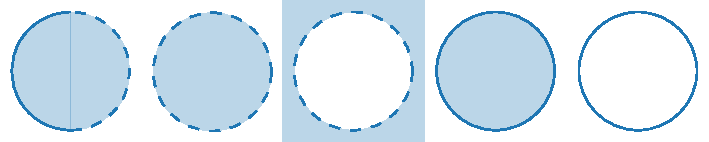
\includegraphics{figures/diagrams/set_properties.pdf}
    \caption{From left to right: \(S\), \(\inte S\), \(\ext S\), \(\closure{S}\), \(\boundary S\).}
\end{figure}

\subsection{Continuity \& Convergence}

The two most important notions in topology are those of \emph{continuous functions} and \emph{sequential convergence}.

% A topology allows us to discuss a series notions commonly discussed in relation to metric spaces without that additional structure. Some of these are \textit{locality, convergence, continuity, compactness, paracompactness, denseness}, along with a others.

% A property of a topological space is said to hold \emphmarginnote{locally} if it is true for one of the following two cases:
% \1 Each point has a neighbourhood exhibiting the property.
% \2 Each point has a neighbourhood basis of sets exhibiting the property
% \0
% Condition 2 is much stronger than condition 1.


Continuous functions between two topological spaces preserve in one direction the structure of the topology of the two spaces.
% \begin{definition}[Continuous functions]
%     A function \(f: X\to Y\) between two topological spaces \(\del{X, \topo{X}}\) and \(\del{Y, \topo{Y}}\) is said to be continuous if for every open set \( V \in \topo{Y}\), its preimage is open in \(X\), \(f^{-1}(V) \in \topo{X}\).
% \end{definition}
A function \(f: X\to Y\) between two topological spaces \(\del{X, \topo{X}}\) and \(\del{Y, \topo{Y}}\) is said to be \emphmarginnote{continuous} if for every open set \( V \in \topo{Y}\), its preimage is open in \(X\), \(f^{-1}(V) \in \topo{X}\).
\begin{figure}[h]
    
\includegraphics{figures/tex/continuous.tex}
\end{figure}
Compositions of continuous functions are continuous, and so are their restrictions to open sets. Continuity can be proved by proving continuity just for a basis on \(\topo{Y}\).

If a bijective function and its inverse are both continuous, then that function is said to be a \emphmarginnote{homeomorphism}, as it preserve the topological structure of the two spaces. If there exists a homeomorphism between \(X\) and \(Y\) then we say that \(X\) and \(Y\) are \emphmarginnote{homeomorphic}, denoted \(X \isomtop Y\) (isomorphic in the topological sense).

A weaker but important notion is that of a \emphmarginnote{local homeomorphism}. A function \(f\) is a local homeomorphism if for every point \(x\in X\) has a neighbourhood \(U\) such that the restriction of \(f\) to \(U\), \(\eval{f}_U\), is a homeomorphism from \(U\) to \(f(U)\). If there exists a local homeomorphism between \(X\) and \(Y\) then we say they are \emphmarginnote{locally homeomorphic}.

Convergence in the topological sense implies a sequence becomes arbitrarily close to a point in the sense of neighbourhoods of the point.
% \begin{definition}[Convergence]
%     The point \( x \in X \) is said to be the limit of a sequence \(\cbr{x_i}_{i=0}^\infty\) if for every neighbourhood \(U\) of \( x \), there is and \(N_U \in \N\) such that for all \( i > N_U \), \( x_i \in U\).
% \end{definition}
The point \( x \in X \) is said to be the \emphmarginnote{limit of a sequence} \(\cbr{x_i}_{i=0}^\infty\) if for every neighbourhood \(U\) of \( x \), there is and \(N_U \in \N\) such that for all \( i > N_U \), \( x_i \in U\). Alternatively we might say that \(\cbr{x_i}_{i=0}^\infty\) \emphmarginnote{converges} to \(x\), denoted \(\cbr{x_i}_{i=0}^\infty x\) or even \(x_i \to x\) for short.
\begin{figure}[h]
    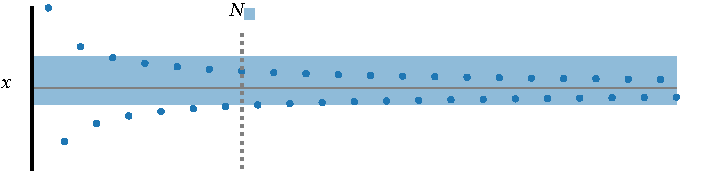
\includegraphics{figures/diagrams/neighbourhood.pdf}
    \caption{The sequence \(\cbr{
\includegraphics{figures/diagrams/tab_blue_scatter.pdf}_i}\) converges to the point \(x\). We see that on the neighbourhood 
\includegraphics{figures/diagrams/tab_blue_fill.pdf}, for \(i > N_{
\includegraphics{figures/diagrams/tab_blue_fill.pdf}}\), \(
\includegraphics{figures/diagrams/tab_blue_scatter.pdf}_i \in 
\includegraphics{figures/diagrams/tab_blue_fill.pdf}\)}
\end{figure}

A set \(S\) is is said to be \emphmarginnote{sequentially closed} if it contains the limits of all sequences in \(S\). This notion is \emph{different} ot that of \emph{topologically closed} introduced earlier, and is different to the notion of containing all of its \emph{topological limit points}. Topological closure implies sequential closure, but not the converse.

A useful combination of these notions is the convergence of sequences under continuous maps. If a sequence \(x_i \to x\), and we have \(f: X\to Y\) continuous, then \(f(x_i) \to f(x)\).

\subsection{"Goldylocks" topologies}
The definition of a topology along with the notions we have introduced can sometimes lead to paradoxical results. On one end if we endow \(X\) with the topology with the least sets, the \emphmarginnote{trivial topology}, \(\topo{X} = \cbr{X, \emptyset}\), then every sequence converges to every point in \(X\). By contrast if we endow \(X\) with the \emphmarginnote{discrete toplopgy}, the topology tha defines \emph{every} subset of \(X\) as open, then it is \emph{totally disconnected}, i.e. that every point is completely separated from every other point. In order to avoid these pathologies in "nice" spaces, we introduce a some more notions so that our topologies have the right amount of open sets to be useful to us. 

A \emphmarginnote{Hausdorff space} ensures that we have \emph{enough} open sets in our topology. A space is said to be Hausdorff if for any two points \(x_1, x_2 \in X\), we can find two open sets \(U_1, U_2\) such that \(x_1 \in U_1\), \(x_2 \in U_2\), but \(U_1 \cap U_2 = \emptyset\). Intuitively this says if I have any two points, I can always separate them into two distinct neighbourhoods. Being a {Hausdorff space} implies two very useful properties:
\1 Every 1-point set \(\cbr{x}\) is closed.
\2 If a sequence \(\cbr{x_i}\) in \(X\) converges to a limit \(x\), then this limit is \emph{unique}.
\0
On a finite set, only the discrete topology is Hausdorff. On infinite sets, many might be. The Hausdorff property is no the only possible "separability" criteria, it exists in a scale of strictness, but it is the most useful to us.

Secondly we have the notion of \emphmarginnote{countability}. This ensures we don't have \emph{too many} open sets in our topology. To introduce this, we first introduce the notion of a \emph{basis} of a topology.

A topology can often be constructed by specifying some special set of open sets, and "completing" this in a suitable manner.
% \begin{definition}[Basis]
%     A basis \(\c{B}\) of \(X\) is a collection of subsets such that their union is \(X\), and for all \(B_1, B_2 \in \c{B}\), there is a \(B_3 \in \c{B}\) such that \(B_3 \subset B_1 \cap B_2\)
% \end{definition}
A \emphmarginnote{basis} \(\c{B}\) of \(X\) is a collection of subsets such that their union is \(X\), and for all \(B_1, B_2 \in \c{B}\), there is a \(B_3 \in \c{B}\) such that \(B_3 \subset B_1 \cap B_2\).

A basis can be completed into a topology by adding to it all possible unions of the sets in the basis. This topology is said to be \emph{generated} by the basis. Bases are useful as they give us something \emph{simpler} from which we can reconstruct the whole topology.

In some sense opposite, we have the notion of a \emphmarginnote{neighbourhood basis}. If we consider \emph{all} the neighbourhoods of a point or set, \(\c{N}(x)\), then a neighbourhood basis \(\c{B}\) is a subset of \(c{N}(x)\) such that for any neighbourhood \(U \in \c{N}(x)\) there is an element in the neighbourhood basis \(V \in \c{B}\) such that \( V \subset U\). This says that for any neighbourhood we can find a set in the neighbourhood basis that is contained within it. This is useful as it allows us to study properties only "very close" to the point, forgetting about the rest of the topology.

In the discrete topology, the set \(\cbrcolon{\cbr{x}}{x\in X}\) is a basis and the set \(\cbr{x}\) is a neighbourhood basis of \(x\) as all points are separated from each other.

A space is \emphmarginnote{first-countable} if every point has a countable neighbourhood basis. First countability implications regarding \emph{sequential closure} and \emph{topological closure}. Previously we had that topological closure \(\implies\) sequential closure, but topological closure \(\centernot\implies\) sequential closure. First countability results in topological closure \(\iff\) sequential closure, i.e. the topological and sequential notions of closure become identical. Every metric space is first countable, but not necessarily the converse.

A space is \emphmarginnote{second-countable} if its topology has a countable basis. Second countability implies first countability, as it must contain a countable neighbourhood basis for each point.

This condition is often used to reduce the number of sets on needs to "cover" a space \(X\). A collection of subsets \(\c{U}\) is called a \emphmarginnote{cover} of \(X\) if for every point in \(X\), there is a \(U \in \c{U}\) such that \(x \in U\). An \emphmarginnote{open cover} is a cover where all the subsets are open. A \emphmarginnote{subcover} is a subset of a cover that remains still a cover. In a second countable space, every open cover of the space has a \emph{countable} subcover.

% Most reasonable spaces we deal with are Hausdorff and second countable. Importantly these properties both hold of Euclidean space. For any two points \(x_1, x_2\) in \(\R^n\) separated by distance \(r\), the open ball neighbourhoods \(B_{\bar{r}}(x_1), B_{\bar{r}}(x_2)\), \(\bar{r} < r/2 \), and so it is Hausdorff. The topology can be generated by the basis of open balls \(\c{B} = \cbrcolon{B_r(x)}{r \text{ is rational and } x \text{ has rational coordinates}}\)


\subsection{Constructing topologies}

Many import spaces can be constructed out of other spaces. When doing this we need to define the topology on these new spaces. 4 examples of particular importance are: \emph{subspaces}, \emph{products}, \emph{disjoint unions} and \emph{quotients}. We will choose canonical ways to define these new topologies that preserve sensible properties on the new spaces.

\subsubsection{Subspaces}

If we have \(S \subseteq X\), then the \emphmarginnote{subset topology} is the topology \(\topo{S} = \cbrcolon{U \^ S}{U \in \topo{X}} = S \^ \topo{X}\), i.e the intersection of the topology of \(X\) with \(S\). We define the \emphmarginnote{inclusion map} \(\inclusion_S:  S \hookrightarrow X\) as the restriction of the identity of \(X\) to \(S\), \(\eval{\id}_S\).

A continuous, \emph{injective} map \(f: X\to Y\) is called a \emphmarginnote{topological embedding} if it is a homeomorphism onto its image in \(Y\), \(f(X) \subseteq Y\), endowed with the subspace topology.

This definition is motivated by the \emphmarginnote{characteristic property of the subset topology}: if \(Y\) is a topological space, \(f: Y \to S\) is continuous if and only if the composition \[Y\xrightarrow{f}S\xhookrightarrow{\inclusion_S}X \] is continuous. The subset topology is the unique topology satisfying this property.
% \(\inclusion_S\circ f: Y \to X\)

This induces a number of properties with respect to \(\topo{X}\) and the subset topology on \(S\), \(S\^ \topo{X}\):
\begin{enumerate}[noitemsep]
    \item The inclusion map is a topological embedding.
    \item The closed subsets of \(S\) are the intersection of the closed subsets of \(X\) with \(S\).
    \item If \(f: X \to Y\) is continuous, then \(\eval{f}_S: S \to Y\) is continuous.
    \item If \(\basis\) is a basis of \(X\), then \(\basis_S = \cbrcolon{B\^S}{B \in \basis}\) is a basis of \(S\).
    \item If we have \(T \subset S \subset X\) then the topology \(T\^ \del{S\^ \topo{X}}\) agrees with \(T\^ \topo{X}\).
    \item If \(X\) is Hausdorff, then \(S\) is Hausdorff.
    \item If \(X\) is first countable, then \(S\) is first countable.
    \item If \(X\) is second countable, then \(S\) is second countable.
\end{enumerate}
The converse of 3. allows us to show that \emphmarginnote{continuity is local}. If we have \(f: X\to Y\), and for every point \(x\in X\) we have a neighbourhood \(U\) such that \(\eval{f}_U\) is continuous, then \(f\) is continuous.

Alternatively, we can \emphmarginnote{glue continues maps} together. If we have a) \(B_1,...,B_n\), a finite collection of closed sets or b) \(\cbr{B_i}_{i\in A}\), any collection of open sets such that \(\u_{a\in A}B_a = X\), and a continuous function for each \(B\), \(f_i: B_i \to Y\), and these functions agree on intersections, \(f_i(B_i \^ B_j) = f_j(B_i \^ B_j)\), then there is a unique continuous function \(f: X\to Y\) such that \(\eval{f}_{B_i} = f_i\). A important corollary of this is that to check continuity it is sufficient to check continuity on a basis of \(X\).

\subsubsection{Product spaces}

Now consider the product of a finite collection of spaces \(X_1, ..., X_n\). Define a basis by \[\basis  = \cbrcolon{U_1 \times ... \times U_n}{U_i \in \topo{X_i}, i=1,..,n}\], the Cartesian product of each combination of sets from each topology. The topology generated by this basis is the \emphmarginnote{product topology}.

The \emphmarginnote{characteristic property of the product topology} is that, for any topological space \(Y\), \(f: B\to X_1\times ... X_n\) is continuous if and only if the composition with each projection function \(\pi_i: x_1, ..., x_n \mapsto x_i\), \(f_i = \pi_i \circ f\) is continuous. The product topology is the unique topology for which this holds.

This induces a number of properties with respect to product topology on \(X_1\times... \times X_n\):
\begin{enumerate}[noitemsep]
    \item Each projection map \(\pi_i\) is continuous.
    \item For continuous functions \(f_i: X_i \to Y_i\), the \emphmarginnote{product map} \(f_1 \times ... \times f_n: X_1 \times .. \times X_n \to Y_1\times ... \times Y_n\), \(f(x_1, ..., x_n) = (x_1, ..., x_n)\) is continuous.
    \item If we have subspaces \(S_i \subseteq X_i\), then the product topology \(S_1\^\topo{X_1} \times ... \times S_n\^\topo{X_n}\) coincides with the subspace topology \((S_1\times ... \times S_n) \^ \topo{X_1 \times ... \times X_n}\).
    \item For any \(i\), and picking \(a_j \in X_j, i\neq j\), then the map \(x \mapsto (a_1, ..., x, ..., a_n)\) it a topological embedding into the product space \(X_1 \times ... \times X_n\).
    \item If \(\basis_i\) is a basis for each \(X_i\), then \(\basis \cbrcolon{B_1 \times ... \times B_n}{B_i\in \basis_i}\) is a basis of \(X_1 \times ... \times X_n\).
    \item Every finite product of Hausdorff spaces is Hausdorff.
    \item Every finite product of first countable spaces is first countable.
    \item Every finite product of second countable spaces is second countable.
\end{enumerate}

For products of an infinite collection of spaces, a piece of subtly creeps in. We want all the properties above to continue to hold. But, as it turns out the basis we defined earlier is not a good choice. On infinite spaces this is known as the \emphmarginnote{box topology}, where we take the products of all the open sets of each space. This topology fails in a number of ways. The box topology fails to preserve compactness through products. For example, functions we expect to be continuous fail to be continuous, and topological convergence becomes a significantly strict condition under the box topology.

Instead we introduce the concept of \emphmarginnote{cylinder sets}. For collection of spaces, each with a collection of subsets, \((X_a, \c{S}_a)_{a\in A}\), we take the Cartesian product of these to give \(X = \prod_{a\in A}\). We get a canonical projection for each \(a\), \(\pi_a: X_a \to X\), that elements of \(X_a\) to its component in \(X\). A \emph{cylinder set} is then a set \[\Int_{i=1}^n \pi_{a_i}^{-1}(S_{a_i}), \quad\quad S_{a_i} \in \c{S}_{a_i}, a_i \in A \]. Note this is a \emph{finite} intersection. Alternatively we can see the cylinder sets as \[\cbrcolon{U_1 \times U_2 \times ...}{U_i \in \topo{X_i}, i=1,2,..., U_i \neq X_i \text{ for finitely many } i}\], products of subsets of each \(X_a\) where only \emph{finitely many} of the subsets are not the whole space \(X_a\).

We then define the \emphmarginnote{product topology on infinite products} to be the one generated by the basis of cylinder sets on the product of \((X_a, \topo{X_a})_{a\in A}\). This topology is the one compatible with the previously stated conditions, and is the default topology on infinite products. In the product topology, topological convergence coincides with the notion of \emphmarginnote{pointwise convergence}, i.e. a sequence of functions converge if and only if each of the component functions \(f_i\) converge.

On finite products, we can see that these two definitions coincide, and so we can use the cylinder sets to define the topology on finite products too.

\subsubsection{Disjoint unions}

An alternative way to join sets together from the Cartesian product is the \emphmarginnote{disjoint union}. For a collection of sets \(\cbr{X_a}_{a\in A}\), the disjoint union is given by appending \(a\) to each element of \(X_a\).\[\coprod_{a\in A} X_a = \cbrcolon{\del{x, a}}{a\in A, x\in X_a}\]. We can define a canonical inclusion map \(\inclusion_a: X_a \to \coprod_{a\in A} X_a\) for each \(a\) by \(\inclusion_a: x \mapsto (x, a)\). We define the open sets of the \emphmarginnote{disjoint union topology} to be the set that when intersected with each \(X_a\), are open in \(\topo{X_a}\). Note this is defined for infinite index sets \(A\).

The \emphmarginnote{characteristic property of the disjoin union topology} is that for a topological space \(Y\), a function \(f: \coprod_{a\in A} X_a \to Y\) is continuous if and only if \(f\circ \inclusion_a \to Y\) is continuous for each \(a\in A\). The disjoint union topology is the unique topology satisfying this property.

This induces a number of properties with respect to disjoint union topology on \(\coprod_{a\in A} X_a\):
\begin{enumerate}[noitemsep]
    \item A subset of \(\coprod_{a\in A} X_a\) is closed if and only if its intersection with each \(X_a\) is closed.
    \item Each injection \(\inclusion_a: X_a \to \coprod_{a\in A} X_a\) is a topological embedding.
    \item Every disjoint union of Hausdorff spaces is Hausdorff.
    \item Every disjoint union of first countable spaces is first countable.
    \item Every disjoint union of second countable spaces is second countable.
\end{enumerate}

\subsubsection{Quotient spaces}

\begin{figure}[h]
    \input{figures/tex/quotient_map.tex}\hfill\documentclass[tikz,10pt]{standalone}
\usepackage[standalone,commands]{../../MJH}

\graphicspath{/Users/mhutchin/Documents/thesis/figures/diagrams/}

% \usepackage{tikz}
% \usetikzlibrary{positioning}

\usepackage{pgfplots}
\pgfplotsset{compat=1.17}
% \usepgfplotslibrary{external}
% \usepgfplotslibrary{groupplots}
% \usepgfplotslibrary{fillbetween}
% \usetikzlibrary{fadings}

\begin{document}
    % \tikzsetnextfilename{generative_model}
    \begin{tikzpicture}
        \node (simple) at (0,0) {
\includegraphics{/Users/mhutchin/Documents/thesis/figures/diagrams/saturated_sets.pdf}};
        \node (math) at (-2.8,-0.3) {\(V\)};
        \node (math) at (3.2,-0.3) {\(U\)};
        \node (math) at (0.225,0.2) {\(S\)};
        \node (math) at (-1.2,-1) {\(\pi(V)\)};
        \node (math) at (1.2,-1) {\(\pi(U)\)};
        \node (math) at (1.4,0.9) {\(\pi^{-1}(S)\)};
        \node (math) at (-1.4,0.9) {\(\neq\pi^{-1}(S)\)};

        % \node (math2) at (-1.5,-1) {\(V\)};

        % \node (math2) at (-1.6,-0.2) {\(U \u V\)};

        % \node (math) at (-0,1.0) {\(\phi_U\)};
        % \node (math) at (-0,-0.7) {\(\phi_V\)};

        % \node (math) at (2.5,0) {\(\phi_V \circ \phi^{-1}_U\)};


        % \node (complex) at (3,0) {
\includegraphics{../diagrams/simple_distribution.pdf}};
        % \draw[-stealth] (math.north) to [out=45,in=135] (math2.north) node [midway, yshift=1.1cm] {\(f\)} ;
        % \draw[-stealth] (math2.west) to (math.east) node [midway, above] {\(f^{-1}(V) = U\)} ;
    \end{tikzpicture}
\end{document}
    \caption[short]{\emph{Left:} The quotient map \(\pi\) maps fibres of blue into points in orange. \emph{Right:} The set \(U\) is a saturated set in blue, as it is the preimage of \(S\). \(V\) is not.}
\end{figure}

Finally we discuss creating quotient spaces. If we have a topological space \(X\), a set \(Y\), and a continuous surjective map \(\pi: X\to Y\), called a \emphmarginnote{quotient map}, then we define the open sets of the \emphmarginnote{quotient topology} \(\topo{Y}\) to be the sets \(U \subseteq Y\) such the preimage \(\pi^{-1}(U)\) is open in \(\topo{X}\). Denote this topology \(\topo{X}\takeaway \pi\).

The most common quotient spaces are induced by an \emphmarginnote{equivalence relation}, \(\sim\). This is a truth operation on two elements on \(X\) such that it is reflexive (\(x\sim x\) for all \(x\in X\)), transitive(\(x\sim y\) and \(y\sim z\) \(\implies x\sim z\)) , and symmetric (\(x\sim y \iff y\sim x\)). We denote the \emphmarginnote{equivalence class} of \(x\), \(\sbr{x}\), as all the elements \(y\) of \(X\) such that \(x\sim y\). The set of all equivalence classes partitions \(X\) into disjoint sets. If we denote the set of all equivalence classes on \(X\) as \(X\takeaway \sim\), then there is a natural quotient map \(\pi: X\to X\takeaway\sim\), \(\pi: x\mapsto \sbr{x}\).

A \emphmarginnote{fibre} of a quotient map \(\pi: X \to Y\) is the preimage of a point in \(Y\), \(\pi^{-1}(y) \subset X\). A \emphmarginnote{saturated set} is a union of fibres. Alternatively, it is a subset \(U \subseteq X\) such that \(U = \pi^{-1}(\pi(U))\).

The \emphmarginnote{characteristic property of the quotient topology} is that, for any quotient map \(\pi : X \to Y\), for any topological space \(B\), a map \(f: Y\to B\) is continuous if and only if the composition \(f \circ \pi : X \to B\) is continuous. The quotient topology is the unique topology satisfying this condition.

This induces a number of properties with respect to quotient topology on \(Y\):
\begin{enumerate}[noitemsep]
    \item \(K \subseteq Y\) is closed if and only if \(\pi^{-1}(K)\) is closed in \(X\).
    \item If \(\pi\) is injective (and therefore bijective), it is a homeomorphism.
    \item If \(U \subseteq X\) is a saturated open or closed set, then \(\eval{\pi}_U: U \to \pi(U)\) is a quotient map.
    \item Any composition of quotient maps is a quotient map.
\end{enumerate}

Importantly, quotient topologies do not necessarily play nicely with products, subspaces or disjoint unions, and do not necessarily preserve the properties of Hausdorff, first or second countability, these have to be checked. 

Quotients have two important properties that will be important later.

\emphmarginnote{Passing to the quotient}. If \(\pi: X\to Y\) is a quotient map, \(B\) a topological space, and we have a continuous function \(f: X\to B\) such that it is \emph{constant} on the fibres of \(\pi\), i.e. that \(\pi(p) = \pi(q) \implies f(p) = f(q)\), then there is a unique continuous map \(\tilde{f}: Y\to B\) such that \(f = \tilde{f}\circ\pi\).

\emphmarginnote{Homeomorphic quotient spaces} can be detected by analysing their quotient maps. If for two quotient maps \(\pi_1: X\to Y_1\) and \(\pi_2: X \to Y_2\) we have that \(\pi_1(p) = \pi_1(q) \iff \pi_2(q) = \pi_2(q)\), then \(Y_1\) and \(Y_2\) are homeomorphic, and there exists a homeomorphism \(\phi: Y_1 \to Y_2\) such that \(\pi_2 = \phi \circ \pi_2\).

\subsubsection{Open and closed maps}
We have now discussed the most important types of continuous maps in topology
\begin{itemize}[nosep]
    \item Homeomorphisms - continuous bijections \(f: X\to Y\) with continuous inverse.
    \item Topological embeddings - continuous injections \(f: X \to Y\) where \(X \subseteq Y\) that are homeomorphisms on their images \(f(X)\) endowed with the subspace topology \(X\^\topo{Y}\).
    \item Quotient maps - continuous surjections \(f: X\to Y\) where \(Y\) is endowed with the quotient topology \(\topo{X}\takeaway f\).
\end{itemize}
It can be hard however when analysing maps between spaces with predetermined topologies,  \((X, \topo{X}), (Y, \topo{Y})\), to determine if maps \(f: X\to Y\) satisfy the conditions above.

An \emphmarginnote{open map} \(f: X\to Y\) is a map such that the image of every open set \(U\subseteq X\), \(f(U)\subseteq\) is open in \(Y\).\\
A \emphmarginnote{closed map} \(f: X\to Y\) is a map such that the image of every closed set \(U\subseteq X\), \(f(U)\subseteq\) is closed in \(Y\).

Using these definitions we can thenprove the following: If \(f: X \to Y\) is an continuous open or closed map then
\begin{itemize}[nosep]
    \item If \(f\) is a bijection, it is a homeomorphism.
    \item If \(f\) is an injection, it is a topological embedding, and \(\topo{X} = X\^\topo{Y}\).
    \item If \(f\) is a surjection, it is a quotient map, and \(\topo{Y} = \topo{X}\takeaway f\).
\end{itemize}

\subsection{Connectedness and Compactness}

% \subsection{Conections}

% \emphmarginnote{Connectedness} tells us if a topological space is split into multiple parts or not. A space is said to be \emph{disconnected} if there exist \(U, V \in \topo{X}\) such that \(U \^ V = \emptyset\) and \(U \u V = X\). A space that is not disconnected is connected.
% \begin{figure}[h]
%     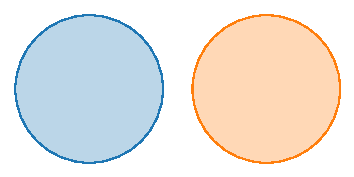
\includegraphics{figures/diagrams/connected_disks.pdf}
%     \caption[short]{The space 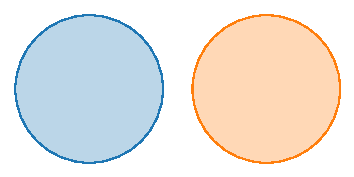
\includegraphics[height=1.5ex]{figures/diagrams/connected_disks.pdf} is disconnected as \(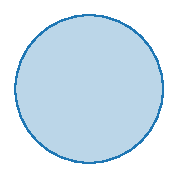
\includegraphics[height=1.5ex]{figures/diagrams/disk_blue.pdf} \^ 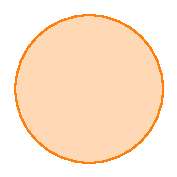
\includegraphics[height=1.5ex]{figures/diagrams/disk_orange.pdf} = \emptyset\) and \(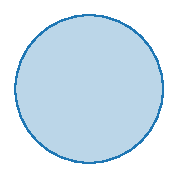
\includegraphics[height=1.5ex]{figures/diagrams/disk_blue.pdf} \u 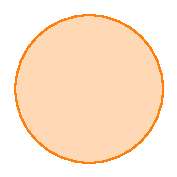
\includegraphics[height=1.5ex]{figures/diagrams/disk_orange.pdf} = 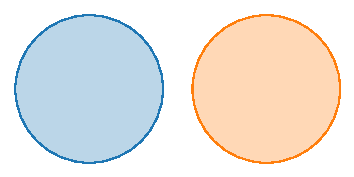
\includegraphics[height=1.5ex]{figures/diagrams/connected_disks.pdf}\)}
% \end{figure}

% A useful corollary of this is that a space is connected if and only if the only two sets in the topology that are both closed and open are \(X\) and \(\emptyset\).

% For any space that is not connected, we can turn this into a series of connected spaces by breaking it into its components. We do this by applying an equivalence relation \(p \tilde q\) if there is a connected subset of \(X\) that contains \(p\) and \(q\). The equivalence class of \(X\) under this equivalence are called the \emph{components} of \(X\), and each is connected. 

% \emphmarginnote{Path connectedness} is a stronger notion than connectedness that implies connectedness. A space is path connected if for every \(p, q \in X\), there is a continuous map \(f: \sbr{0,1} \to X\).
% \begin{figure}[h]
%     \centering
%     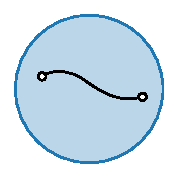
\includegraphics{figures/diagrams/continuous_path.pdf}\hspace{1cm}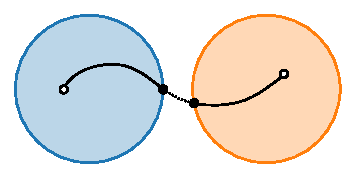
\includegraphics{figures/diagrams/discontinuous_path.pdf}
%     \caption{The space on the left is path connected, the space on the right is not.}
% \end{figure}

\section{Manifolds}
\subsection{Topological Manifolds}
With all this in place, we are ready to define a manifold.
\begin{definition}[Topological manifold]
    An n-dimension topological manifold is a \emph{Hausdorff} and \emph{second-countable} topological space for which \emph{every point has a neighbourhood homeomorphic to an open subset of \(\R^n\)}.
\end{definition}
This last condition is alo stated as being \emph{locally Euclidean of dimension \(n\)}. Note that the requirement of second countability is sometimes replaced with \emphmarginnote{paracompactness}. In locally Euclidean Hausdorff spaces, these two notions imply each other and so this is a moot point. This means therefore a manifold \(X\) is in fact a tuple \(\del{X, \topo{X}}\), containing a set along with a suitable topology.

Euclidean space of dimension n is clearly a topological manifold of dimension n, when endowed with the topology induced by the usual Euclidean metric.

We call any open subset of \(X\) along with the homeomorphism \(\phi: U \to \underset{\text{open}}{\subset} \R^n\) a \emphmarginnote{chart} of \(X\). A collection of charts \(\cbrcolon{\del{U_a, \phi_a}}{a\in A}\) such that \(\underset{a\in A}{\u} U_a = X\) an \emphmarginnote{atlas} of \(X\), denoted \(\atlas{X}\). For any two charts \(\del{U, \phi_U}, \del{V, \phi_V}\) in an atlas where \(U\^ V \neq \emptyset\) we can define the \emphmarginnote{transition map} between them as the map \(\phi_{UV}: \phi_{U}(U\^V) \to \phi_V(U\^ V)\) as the composition \(\phi_{UV} = \phi_V \circ \phi_U^{-1}\). An atlas is called a \emphmarginnote{maximal atlas} if it is not a subset of some larger atlas. 

We may also be interested in manifolds that have \emph{edges}, aptly names manifolds with boundary.
\begin{definition}[Manifold with boundary]
    An n-dimension topological manifold with boundary is a \emph{Hausdorff} and \emph{second-countable} topological space for which every point has a neighbourhood homeomorphic to an open subset of the n-dimension \(\mathbb{H}^n\).
\end{definition}
where \(\mathbb{H}^n\) is the \emphmarginnote{upper half-space}, \(\mathbb{H}^n = \cbrcolon{\del{x_1, ..., x_n}\in\R^n}{x_n \geq 0}\). We call any point that has a neighbourhood homeomorphic to the upper half-space a \emphmarginnote{boundary point}, and denote the collection of these the \emphmarginnote{boundary}, denoted \(\partial X\). Points that are not boundary points are call \emphmarginnote{interior points}.
\begin{figure}[h]
    % 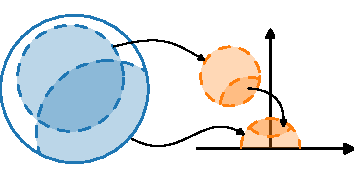
\includegraphics{figures/diagrams/boundary_charts2.pdf} % 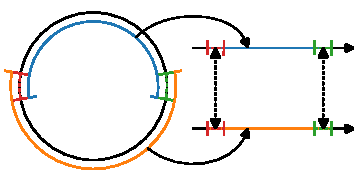
\includegraphics{figures/diagrams/circle_atlas.pdf}
    \input{figures/tex/boundary_chart.tex}
    \caption{Two charts of the atlas \(\atlas{X}\) of \(X\), the unit disk, a manifold with boundary. \(\del{U, \phi_U}\), a chart mapping into a subset of \(\R^n\), and \(\del{V, \phi_V}\), a chart mapping into a subset of the upper half-space \(\mathbb{H}^2\).}
\end{figure}
\begin{figure}[h]
    
\includegraphics{figures/diagrams/earth.pdf}\hspace{1cm}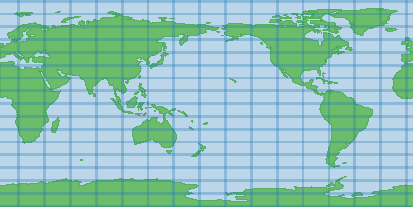
\includegraphics{figures/diagrams/earth_flat.pdf}
    \caption{The projection of the earth onto a flat map is the prototypical example of a chart. While the Mercator projection it looks like the chart covers the whole globe, but mathematically it is in fact missing the poles and a line connecting them as we need the set to be an open one.}
\end{figure}

The required structure of a manifold (with boundary) implies additional properties: all topological manifolds (with boundary) are locally path-connected, locally compact, and paracompact.

Using the previously outlined ways of producing topological spaces from other topological spaces, it is clear we can create new manifolds automatically via taking subspaces of manifolds, taking products of manifolds, or by taking direct products of manifolds. We can also produce new manifolds via quotients, however we must check that this quotient preserves the Hausdorff and second countable properties manually.

While not required for the definition of a manifold, the concept of charts and atlases is key to the study of additional structure we can impose on a manifold. In addition, from a computational perspective they are incredibly useful as they give us one way of representing points on a manifold as a series of real numbers.%.The first such additional structure we will explore is that of \emph{smoothness}. We briefly review some concepts of vector spaces, linear algebra, and calculus. 

\subsubsection{Examples}

\subsection{Smooth manifolds}

A smooth manifold is a topological manifold with additional structure. In this case, we want to ensure that the charts and transition maps of the atlas of the manifold as \emph{smooth}. For a chart \((U, \phi)\) to be smooth we require that \(\phi: U \to \R^k\) be smooth (\(\phi\in C^\infty\)), if all its component functions have continuous differentials of all orders. An atlas is said to be \emphmarginnote{smoothly compatible} is for every pair of charts \((U, \phi), (V, \psi)\) the transition maps \(\phi \circ \psi^{-1}\) and \(\psi \circ \phi^{-1}\) restricted to \(\phi(U\^V)\) and \(\psi(U\^V)\) are smooth. A \emphmarginnote{smooth structure} on \(X\) is a \emph{maximal smooth atlas}, and so a \emphmarginnote{smooth manifold (with boundary)} is a triple \((X, \topo{X}, \atlas{X})\) with the right properties. Every coordinate chart of a smooth manifold is itself smooth.

Showing a manifold is smooth is not always simple from the definition. The following is useful as it lets us create a smooth manifold with suitable charts:
\begin{lemma}[Smooth manifold chart lemma]
    \label{lem:smooth_chart}
    Suppose \(X\) is a set, and we have a subset of collections \(\cbr{U}_a\) along with maps \(\phi_a: U\to \R^n\). If the following are satisfied:
    \1 for each \(a\), \(\phi_a\) is a bijection between \(U_a\) and an \emph{open} subset of \(\R^n\) with the usual topology.
    \2 For each \(a\), \(b\), the sets \(\phi_a(U_a\^U_b)\) and \(\phi_b(U_a\^U_b)\) are open in \(\R^n\) with the usual topology.
    \3 For all \(a,b\) where \(U_a\^U_b \neq \emptyset\), the map \(\phi^{-1}_a\circ\phi_b: \phi_a(U_a\^U_b) \to \phi_b(U_a\^U_b)\) is smooth.
    \4 Countably many \(U_a\) cover \(X\).
    \5 When \(p, q\in X\), \(p\neq q\), there exists some \(U_a\) containing \(p\) and \(q\), or there exist disjoint \(U_a, U_b\) with \(p\in U_a\), \(q\in U_n\).
    \0
    Then \(X\) has a unique smooth manifold structure such that each \((U_a, \phi_a)\) is a smooth chart. 
\end{lemma}
\begin{proof}
    \cite[p.22]{lee2013smooth}
\end{proof}
The topology of the structure is induced by the topology on \(\R^n\) and the \((U_a, \phi_a)\) (1-3). The basis for the topology on \(X\) is given by \(\basis = \cbrcolon{\phi_a^{-1}(S)}{S \text{ is open in } \phi_a(U_a) \text{ for all  } a}\). 4. ensures second countability, and 5. Hausdorff.

We can define \emphmarginnote{smooth functions on manifolds}. \(f: X\to \R^k\) is a smooth function if for every point \(p \in X\) and chart \((U, \phi) \in \atlas{X}\) the function \(f \circ \phi^{-1}: \phi(U)\to \R^k\) is smooth. Typically we denote the space of smooth function \(f: X\to \R^k\) as \(C^\infty(X, \R^k)\), and \(f: X\to \R\) \(C^\infty(X)\). Like continuity, smoothness is a local property, and it suffices to check that for a sub-atlas of the atlas on a smooth manifold that a function is smooth on the restriction ot each chart to show it is globally smooth.

The space of functions \(C^\infty(M)\) forms a vector space over \(\R\) using pointwise addition and pointwise multiplication of scalars as the vector space operations. If we add pointwise multiplication (but \emph{not} division), this turns \(C^\infty(M)\) into both a \emph{commutative ring} and a \emph{commutative and associative algebra}.

We can define \emphmarginnote{smooth functions between manifolds} as well. \(f: X \to Y\), where \(X, Y\) are smooth manifolds, is smooth if for each pair of charts \((\phi, U)\in \atlas{X}, (\psi, V) \in \atlas{Y}\) the composition \(\psi \circ f \circ \phi^{-1}: \phi(U)\to \psi(V)\) is smooth. We denote the space of smooth functions between \(X\) and \(Y\) as \(\C^\infty(X, Y)\). A \emphmarginnote{diffeomorphism} between manifolds is a smooth bijection with smooth manifolds. A pair of manifolds for which a diffeomorphism exists are said to be \emphmarginnote{diffeomorphic}, \(X \isomdiff Y\).

\begin{figure}[h]
    \documentclass[tikz,10pt]{standalone}
\usepackage[standalone,commands]{../../MJH}

\graphicspath{/Users/mhutchin/Documents/thesis/figures/diagrams/}

% \usepackage{tikz}
% \usetikzlibrary{positioning}

\usepackage{pgfplots}
\pgfplotsset{compat=1.17}
% \usepgfplotslibrary{external}
% \usepgfplotslibrary{groupplots}
% \usepgfplotslibrary{fillbetween}
% \usetikzlibrary{fadings}

\begin{document}
    % \tikzsetnextfilename{generative_model}
    \begin{tikzpicture}
        \node (simple) at (0,0) {
\includegraphics{/Users/mhutchin/Documents/thesis/figures/diagrams/hom_not_diff.pdf}};
        \node (math) at (0, 0.5) {\(\isomtop\)};
        \node (math) at (0, -0.5) {\(\not\isomdiff\)};
    \end{tikzpicture}
\end{document}
    \caption{Diffeomorphism is a stronger condition that homeomorphic. The disk is homeomorphic to the square, but not diffeomorphic, as one runs into smoothness difficulties with the sharp corners.}
\end{figure}

\subsection{Tangent vectors and tangent spaces}

One of the key advantages of studying smooth manifolds is that it allows us to bring the notions of calculus to the study of manifolds. The most basic concept is that of the \emph{tangent vector}.

We can begin looking at tangent vectors on manifolds by first looking at tangent vectors on \(\R^n\). Since all we have defined on smooth manifolds so far is smooth functions and smooth charts, we will need a definition that works in terms of these. Consider the set \(\R^n_p = \cbr{p}\x \R^n\). We will call this the \emphmarginnote{geometric tangent space} at \(p\). We call an element of this, \((p, v), \; v\in \R^n\), usually written at \(\eval{v}_p\) or \(v_p\), a \emphmarginnote{geometric tangent vector}. This is clearly a vector space with operations \[v_p + w_p = (v + w)_a \quad\quad c(v_p) = (cv)_p\]. The subscript \(p\) is to allow us to differentiate between tangent spaces at different points \(p\) and \(q\). Given the canonical basis of \(\R^n\), \(e_1, ...., e_n = (1, ..., 0), ..., (0, ..., 1)\), we can put a natural basis on \(\R^n_p\) as \(\eval{e_1}_p = (p, e_1), ..., \eval{e_n}_p = (p, e_n)\) via the \emphmarginnote{canonical isomorphism} \(\inclusion_p: \R^n \to \cbr{p}\x \R^n\), \(\inclusion_p : v \mapsto (p, v)\).

For a smooth function \(f \in C^\infty(\R^n)\) we can define the \emphmarginnote{directional derivative} \(D_{v_a}: C^\infty(\R^n) \to \R\) as \[ D_{v_a} f = D_v f(a) = \eval{\od{}{t}}_{t=0} f(a + tv) \]. This operation obeys the product rule \[ D_{v_a} (fg) = f(a) D_{v_a}f + g(a) D_{v_a}f \]. For the basis vectors \(\eval{e_i}_p\), \[D_{\eval{e_i}_p} f = \pd{f}{x_i}(p)\], simply the partial derivative with respect to the \(i\)th input. So for \(v_p \in \R^n_p\) expressed as \(v = \sum_{i=1}^n v_i \eval{e_i}_p\), we have that \[D_{v_p} f = \sum_{i=1}^n v_i \pd{f}{x_i}(p)\]
\begin{figure}[h]
    \documentclass[tikz,10pt]{standalone}
\usepackage[standalone,commands]{../../MJH}

\graphicspath{/Users/mhutchin/Documents/thesis/figures/diagrams/}

% \usepackage{tikz}
% \usetikzlibrary{positioning}

\usepackage{pgfplots}
\pgfplotsset{compat=1.17}
% \usepgfplotslibrary{external}
% \usepgfplotslibrary{groupplots}
% \usepgfplotslibrary{fillbetween}
% \usetikzlibrary{fadings}

\begin{document}
    % \tikzsetnextfilename{directional_derivative}
    \begin{tikzpicture}
        \node (simple) at (0,0) {
\includegraphics{/Users/mhutchin/Documents/thesis/figures/diagrams/directional_derivative.pdf}};
    \end{tikzpicture}
\end{document}
    \caption{Directional derivative.}
\end{figure}

Bearing this in mind, we define a \emphmarginnote{derivation at \(p\)} as a linear function \(w: C^\infty(\R^n)\to \R\) that follows the product rule \[w(fg) = f(p) w(g) + g(p) w(f)\]. We denote \(T_p\R^n\) as the space of all derivations of \(C^\infty(\R^n)\) at \(p\). This is a vector space, with the operations \[(w_1 + w_2)f = w_1 f + w_2f \quad \quad (cw) f = c(wf)\]. We can then prove that our geometric tangent vector direction derivative and the derivatives at \(p\) are isomorphic.
\begin{proposition}[\(T_p\R^n \isomvec \R^n_p\)]
    \1 For each \(v_p\in \R^n_p\), \(D_{v_p}\) is a derivation.
    \2 The map \(V_p \mapsto D_{v_p}\) is an isomorphism from \(\R^n_p\) onto \(T_p\R^n\).
    \0
\end{proposition}
\begin{proof}
    \cite[proposition 3.2]{lee2013smooth}
\end{proof}
    
This then give us a natural way to define the \emphmarginnote{tangent space at a point on a manifold}, \(T_pX\), as the vector space of derivations of \(C^\infty(X)\) at \(p\). For a \(n\)-dimension manifold is \(n\)-dimension vector space, isomorphic (in the vector space sense) to \(\R^n\). Intuitively, this is the space of all possible directions one could move in from \(p\).
\begin{figure}[h]
    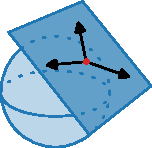
\includegraphics{figures/diagrams/tangent_space_sphere.pdf}
    \caption{The tangent space of the point \(\icon{figures/diagrams/dot_red.pdf}\in \c{S}_2\) with example tangent vectors.}
\end{figure}

If we have a smooth function between manifolds \(F: X\to Y\), we can also define a natural map between their tangent spaces at a point \(p\in X\) and \(F(p)\in Y\), \(\d F: T_pX\to T_{F(p)}Y\), called the \emphmarginnote{differential} of \(F\) at \(p\) by its action on a tangent vector \(v \in T_pX\) and a smooth function on \(Y\), \(f\in C^\infty (Y)\). \[\sbr{\d F_p (v)}\del{f} = v \del{f \circ F}, \quad v\in T_pM, \; f\in C^\infty(Y) \]. This is a \emph{linear} map that distributes over compositions of maps between manifolds, \(\d_p\del{F\circ G} = \d F_{G(p)} \circ \d G_p\), and preserves the identity map, \(\d(\id_X)_p = \id_{T_pX}\). Importantly if \(F\) is a \emph{diffeomorphism}, then \(\d F\) is an \emph{isomorphism} between tangent spaces and \(\del{\d F}^{-1} = \d \del{F^{-1}}\).
\begin{figure}[h]
    \documentclass[tikz,10pt]{standalone}
\usepackage[standalone,commands]{../../MJH}

\graphicspath{/Users/mhutchin/Documents/thesis/figures/diagrams/}

% \usepackage{tikz}
% \usetikzlibrary{positioning}

\usepackage{pgfplots}
\pgfplotsset{compat=1.17}
% \usepgfplotslibrary{external}
% \usepgfplotslibrary{groupplots}
% \usepgfplotslibrary{fillbetween}
% \usetikzlibrary{fadings}

\begin{document}
    % \tikzsetnextfilename{generative_model}
    \begin{tikzpicture}
        \node (simple) at (0,0) {
\includegraphics{/Users/mhutchin/Documents/thesis/figures/diagrams/differential.pdf}};
        \node (math) at (-3.3,-0.85) {\(X\)};
        \node (math) at (3.3,-0.7) {\(Y\)};
        \node (math) at (-.7,-1.3) {\(F\)};
        \node (math) at (-.7,.8) {\(\d F_p\)};
        \node (math) at (-2.3,.8) {\(v\)};
        \node (math) at (1.3,0.85) {\(\d F_p (v)\)};
        \node (math) at (-2.6,.2) {\(p\)};
        \node (math) at (1.2,.05) {\(F(p)\)};
    \end{tikzpicture}
\end{document}
    \caption{A smooth map between smooth manifolds \(F: X \to Y\) induces a natural map between the tangent spaces of \(p\) and \(F(p)\), the differential \(\d F_p\).}
\end{figure}

\subsection{Local coordinates}

The concepts of tangent vectors and differentials just introduced are very abstract. To understand them better, and make them computationally useful, we can introduce the concept of \emphmarginnote{coordinate vectors}.

For the special case of \(\R^n\), we already know how to define a basis on the tangent space at \(p\in \R^n\), \(T_p\R^n\). We simply take the partial differentials with respect to each input at the given point, \(\eval{\pd{}{x_1}}_p, ..., \eval{\pd{}{x_n}}_p\). Any derivation  can then be expressed as \[v = \sum_{i=1}^n v^i \eval{\pd{}{x_i}}_p \quad\quad v \in T_p\R^n ,\; v_i \in \R\]. Their action on a smooth function \(f\in C^\infty(\R^n)\) is simply \[\eval{\pd{}{x_i}}_p \del{f} = \pd{f}{x_i}\del{p}\]

Using this basis on \(T_p\R^n\), we can place a basis on a tangent space of a manifold \(T_pX\) at point using a smooth chart \((U, \phi)\in \atlas{X}\) containing that point. Remember that a smooth chart \(\phi: U \to \R^n\) is a diffeomorphism onto its image. Therefore, the differential \(\d \phi_p: T_pX \to T_{\phi(p)}\R^n\) is an isomorphism. We can define a basis on \(T_pX\) then as the \emph{preimage} of the standard basis on \(T_{\phi(p)}\R^n\) under \(\phi\). Let us then define the basis vector \[\eval{\pd{}{\phi_i}}_{ p} = \del{\d \phi_p}^{-1} \del{\eval{\pd{}{x_i}}_{\phi({p})}} = d\del{\phi^{-1}}_{\phi(p)}\del{\eval{\pd{}{x_i}}_{\phi({p})}}\]. Often, \(\eval{\pd{}{\phi_i}}_{p}\) is denoted as \(\eval{\pd{}{x_i}}_{p}\), obscuring the dependence on \(\phi\) and potentially confusing it with the basis vector of \(T_{\phi(p)}\R^n\) that it is related to, \( \eval{\pd{}{x_i}}_{\phi(p)}\). For further simplicity, the notation is often shortened further to \[\eval{\pd{}{\phi_i}}_{p} = \eval{\partial \phi_i}_p = \eval{\partial x_i}_p = \eval{\partial_i}_p\] when the chart and local coordinates are implied. The action of one of these basis vectors on a function \(f\in C^\infty(X)\) is then \[\eval{\pd{}{\phi_i}}_{p}f = \eval{\pd{}{x_i}}_{\phi(p)} \del{f \circ \phi^{-1}}\]. We can then express any tangent vector \(v \in T_pX\) as \[v = \sum_{i=1}^n v_i \eval{\pd{}{\phi_i}}_p \quad\quad v \in T_pX ,\; v_i \in \R \]
\begin{figure}[h]
    \documentclass[tikz,10pt]{standalone}
\usepackage[standalone,commands]{../../MJH}

\graphicspath{/home/mhutchin/GoogleDrive/University - Postgraduate/Theses/Final/figures/diagrams/}

% \usepackage{tikz}
% \usetikzlibrary{positioning}

\usepackage{pgfplots}
\pgfplotsset{compat=1.17}
% \usepgfplotslibrary{external}
% \usepgfplotslibrary{groupplots}
% \usepgfplotslibrary{fillbetween}
% \usetikzlibrary{fadings}

\begin{document}
    % \tikzsetnextfilename{generative_model}
    \begin{tikzpicture}
        \node (simple) at (0,0) {
\includegraphics{/home/mhutchin/GoogleDrive/University - Postgraduate/Theses/Final/figures/diagrams/tangent_basis.pdf}};
        \node (math) at (-4.5,-0.3) {\(U \subset X\)};
        \node (math) at (-1.8,-1.7) {\(\phi\)};
        \node (math) at (-1.4,-0.75) {\(\d \phi_p\)};
        \node (math) at (4.5,-1.) {\(Y \subset \R^n\)};
        \node (math) at (1.4,0.1) {\(T_{\phi(p)}\R^n\)};
        \node (math) at (-3.8,1.1) {\(T_{p}X\)};
        \node (math) at (-3.1,.4) {\(p\)};
        \node (math) at (0.1,.8) {\(\phi(p)\)};
        \node (math) at (-2.,.6) {\(\eval{\partial\phi_\text{lon}}_{p}\)};
        \node (math) at (-2.9,1.3) {\(\eval{\partial\phi_\text{lat}}_{p}\)};
        \node (math) at (1.85,.85) {\(\eval{\partial x_\text{lon}}_{\phi(p)}\)};
        \node (math) at (1.2,1.4) {\(\eval{\partial x_\text{lat}}_{\phi(p)}\)};
        \node (math) at (4.7,0.05) {\(x_\text{lon}\)};
        \node (math) at (3.3,1.4) {\(x_\text{lat}\)};
        % \node (math) at (1.2,.05) {\(F(p)\)};



        % \node (math2) at (-1.5,-1) {\(V\)};

        % \node (math2) at (-1.6,-0.2) {\(U \u V\)};

        % \node (math) at (-0,1.0) {\(\phi_U\)};
        % \node (math) at (-0,-0.7) {\(\phi_V\)};

        % \node (math) at (2.5,0) {\(\phi_V \circ \phi^{-1}_U\)};


        % \node (complex) at (3,0) {
\includegraphics{../diagrams/simple_distribution.pdf}};
        % \draw[-stealth] (math.north) to [out=45,in=135] (math2.north) node [midway, yshift=1.1cm] {\(f\)} ;
        % \draw[-stealth] (math2.west) to (math.east) node [midway, above] {\(f^{-1}(V) = U\)} ;
    \end{tikzpicture}
\end{document}
    \caption{Using a chart on the sphere that maps from points on the sphere to their latitude and longitude, we can induce a basis on the tangent space on the sphere in the latitude and longitude direction via the differential of the chart.}
\end{figure}
\begin{figure}[h]
    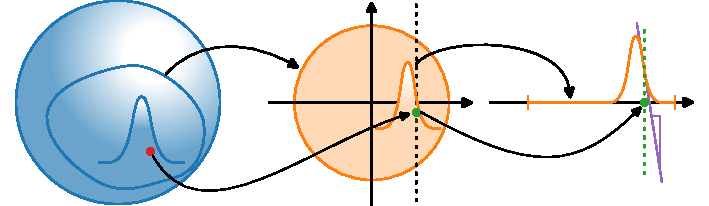
\includegraphics{figures/diagrams/coordinate_differential.pdf}
    \caption{Taking the differential of \(f\), a bump function, evaluated at \(p\) in the i'th direction. Push the function \(f\) onto the chart \(U\) through \(\phi\) to give the function \(f\circ \phi^{-1}: \R^k\to \R\). Then restrict this function to the i'th component to give \(\eval{f\circ \phi^{-1}}_i: \R \to \R\). Finally, evaluate the derivative of this as usual, in purple here at the i'th coordinate of \(\phi(p)\).}
\end{figure}

We can also study how the differential behaves in local coordinates. First again let us consider the special case of \(F: U\subseteq\R^n \to V\subseteq\R^m\), with the standard basis for the tangent spaces \(\eval{\pd{}{x_1}}_p, ..., \eval{\pd{}{x_n}}_p\) and \(\eval{\pd{}{y_1}}_q, ..., \eval{\pd{}{y_m}}_q\). Applying the definition of the differential and the chain rule to a function \(f\in C^\infty (\R^m)\), we get \[\d F_p\del{\eval{\pd{}{x_i}}_p}f = \eval{\pd{}{x_i}}_p \del{f \circ F} = \sum_{j=1}^m \pd{f}{y_j}\del{F(p)} \pd{F_j}{x_i}(p) = \del{\sum_{j=1}^m  \pd{F_j}{x_i}(p) \eval{\pd{}{y_j}}_{F(p)}} f\]. Therefore \[\d F_p\del{\eval{\pd{}{x_i}}_p} = \sum_{j=1}^m  \pd{F_j}{x_i}(p) \eval{\pd{}{y_j}}_{F(p)} \]. If we have \(v = \sum_{i=1}^n v_i \eval{\pd{}{x_i}}_p\), then its image under the differential, \(w = \d F(v)\) in basis coefficients is \[\begin{bmatrix}
    w_1 \\ \vdots \\ w_m
\end{bmatrix}
    = \begin{bmatrix}
    \pd{F_1}{x_1}(p) & \dots & \pd{F_1}{x_n}(p) \\
    \vdots & \ddots & \vdots \\
    \pd{F_m}{x_1}(p) & \dots & \pd{F_m}{x_n}(p)
\end{bmatrix}\begin{bmatrix}
    v_1 \\ \vdots \\ v_n
\end{bmatrix}\]. So we see in local coordinates the differential is associated with a matrix with entries \(\pd{F_j}{x_i}\). This is exactly the \emphmarginnote{Jacobian matrix} of \(F\). The differential is therefore the coordinate-free definition of the Jacobian.

In order to apply this to the differential of \(F: X \to Y\), we again look at the behaviour with respect to charts. Pick two charts \((U, \phi)\in \atlas{X}\), \(p\in U\), and \((V, \psi)\in \atlas{Y}\), \(F(p)\in V\), and write that \(\tilde{F} = \psi \circ F \circ \phi^{-1}\), so \( F = \psi^{-1} \circ \tilde F \circ \phi\). We know that \(\d \tilde F _{\phi(p)}\) in coordinates is the matrix described above, \(\pd{\tilde F_j}{\x_i}\). We can then write \[\d F_p \del{\eval{\pd{}{\phi_i}}_p} = \d \del{\psi^{-1} \circ \tilde F \circ \phi}_p \del{\eval{\pd{}{\phi_i}}_p} &= \d {\psi^{-1}}_{F(p)} \circ \d {\tilde F}_{\phi(p)} \circ \d {\phi}_p \del{\eval{\pd{}{\phi_i}}_p} \\&= \d {\psi^{-1}}_{F(p)} \circ \d {\tilde F}_{\phi(p)}  \del{\eval{\pd{}{x_i}}_{\phi(p)}} \\ &= \d {\psi^{-1}}_{F(p)} \del{\sum_{j=1}^m \pd{\tilde F_j}{x_i}\eval{\pd{}{y_j}}_{\psi(p)}} \\ &= \sum_{j=1}^m \pd{\tilde F_j}{x_i}\eval{\pd{}{\psi_j}}_{p}\]. So again we see that the differential is associated in local coordinates with the Jacobian matrix \(\pd{\tilde F_j}{x_i}\).

One particular example of the differential in coordinates is in the effect on tangent vectors under a change in chart, called a \emphmarginnote{change in coordinate}. If we have \(p\) in two charts \((U, \phi)\), \((V, \psi)\) and a vector at \(p\), \(v = \sum_{i=1}^n a_i \eval{\pd{}{\phi_i}}_p = \sum_{i=1}^n b_i \eval{\pd{}{\psi_i}}_p\), then the basis coefficients are related by \(b_j = \sum_{i=1}^n \pd{\psi \circ \phi^{-1}_j}{x_i} a_i\). As a small abuse of notation I will write \(\pd{\psi \circ \phi^{-1}_j}{x_i} = \pd{\psi_j}{\phi_i}\). Since we know this differential is an isomorphism, so must its Jacobian, i.e. is it full rank, so \(\pd{\psi_j}{\phi_i}\in \groupGL\). This group that related the basis coefficients of different bases of the tangent space is called the \emphmarginnote{structure group} of the manifold. If we have additional structure on our manifold, we can get a \emphmarginnote{reduced structure group} \(G\subset \groupGL\) by preferring a subset of specific bases on each tangent space. \todo{talk more on structure groups, frame bundles etc? COvered well by weiler.}. For example, if we have a notion of an inner product on the tangent space, we can prefer orthonormal bases and reduce the structure group to \(\groupO\). If our manifold is \emph{orientable} then we can 
 

\begin{figure}[h]
    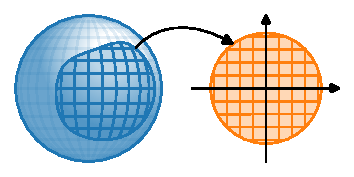
\includegraphics{figures/diagrams/coordinate_chart.pdf}
    \caption{A coordinate chart of the sphere, \(\c{S}_2\).}
\end{figure}

\begin{figure}[h]
    
\includegraphics{figures/diagrams/earth.pdf}
\end{figure}



\subsection{Tangent bundles and vector fields}

We have just considered the tangent space of a point \(p\) on a manifold \(X\). What if we want to consider the tangent space at every point on a manifold simultaneously? This leads us to the notion of the tangent \emph{bundle}.

We construct the \emphmarginnote{tangent bundle} by taking the set \emph{disjoint union} of the tangent spaces, \[TX = \disjointU_{p\in X} T_pX = \cbrcolon{(x, v)}{x\in X, v\in T_xX}\]. Along with this we have a \emphmarginnote{canonical projection} \(\pi : TX \to X\), defined by \(\pi: (x, v) \mapsto x\). The topology we place on this is \emph{not} however the disjoint union topology. The disjoint union topology would leave each tangent space topologically disconnected from each other. Instead, we give it a \emphmarginnote{natural topology} that renders the tangent bundle itself also a manifold of dimension \(2n\). 

\begin{proposition}[The tangent bundle is a smooth manifold]
    For any smooth \(n\)-dimension manifold \(X\), the tangent bundle is a \(2n\)-dimension smooth manifold with a natural topology and smooth structure. With respect to this structure, the projection \(\pi: TX \to X\) is smooth.z 
\end{proposition}

\begin{proof}
To do this, we construct charts that satisfy the smooth chart lemma (\cref{lem:smooth_chart}).

We construct our charts on \(TX\) out of the atlas of the base manifold \(\atlas{X}\). 

Take any chart in \(\atlas{X}\), \((U, \phi)\). We construct a new chart \(\Phi: TU \to \R^{2n}\) (\(TU = \coprod_{p\in U} T_pX\)) by taking the coordinate functions  \(\phi_i: U \to \R\) and the induced basis on the tangent space \(T_pX\), \(\eval{\partial \phi_i}_p\). Defining \[\Phi(p, v^i\eval{\partial \phi_i}_p) = \del{\phi_1(p), ..., \phi_n(p), v_1, ..., v_n}\]. This is a bijection as its inverse is \[\Phi^{-1}(x_1, ..., x_n, v_1, ..., v_n) = \del{\phi^{-1}(x_1, ..., x_n), v^i\eval{\phi_i}_{\phi^{-1}(x_1, ..., x_n)}}\]. For \(\Psi\) constructed similarly to \(\Phi\), the transition function \(\Psi \circ \Phi^{-1}\) is given by \[\Psi \circ \Phi^{-1}(x_1, ..., x_n, v_1, ..., v_n) = \del{\del{\psi\circ\phi^{-1}}(x_1, ..., x_n), \sum_{i=1}^n \pd{\psi_1}{\phi_i} v_i, ..., \sum_{i=1}^n \pd{\psi_n}{\phi_i}v_i} \] which is smooth.

To satisfy the smooth chart lemma:
\begin{enumerate}[noitemsep]
    \item For any chart \((TU, \Phi)\), this is a bijection onto \(\phi(U)\x \R^n \underset{\text{open}}{\subseteq} \R^n \x \R^n\), an open set of \(\R^{2n}\).
    \item Similarly, for \((TU, \Phi)\), \((TV, \Psi)\), \(\Phi(TU\^TV)\) and \(\Psi(TU\^TV)\) are open subsets of \(\R^n\).
    \item The transition maps \(\Psi \circ \Phi^{-1}\) are smooth as shown.
    \item We can pick a countable cover of \(TX\) by taking a countable cover of \(X\) and use those charts to construct our charts on \(TX\).
    \item If we have \((p,v_1), (p, v_2)\) and a set \(p \in U\), then \((p,v_1), (p, v_2) \in TU\). If we have \((p,v), (q, w)\), \(p\neq q\), then from the charts of \(X\) we have \(U, V\) such that they are disjoint and \(p\in U\), \(q \in V\). Therefore \((p, v)\in TU\), and \((q, w)\in TV\), but \(TU, TV\) are disjoint.
\end{enumerate}

To show that \(\pi\) is smooth, note that \(\pi: (x, v) \mapsto x\). In charts \((U, \phi)\), \((TU, \Phi)\) this is simply a restriction to the first half of the coordinates, with is smooth.
\end{proof}

Having constructed our tangent bundle, this allows us to define the notion of a \emphmarginnote{vector field}. In the Euclidean setting, this amounts to continuous map from \(\R^n \to \R^n\) (or open subsets of), that can be visualised as an "arrow" at each point. In the sense of the direction derivative discussed earlier, this akin to attaching a directional derivative to each point.

A \emphmarginnote{vector field on a smooth manifold} is a map \(V: X \to TX\) such that its composition with \(\pi\) is the identity \[\pi \circ V = \id_X\]. In other works, it maps every point to a vector in the tangent vector of that point. We write the value at a point to be \(V_p = V(p)\).

A \emphmarginnote{smooth vector field} is one that is a smooth function between \(X\) and \(TX\). A \emphmarginnote{rough vector field} is one that is not.

We will denote the space of vector fields as \(\Gamma(TX)\). Sometimes it is written as \(\mathfrak{X}(X)\). This is a vector space under pointwise addition and pointwise scalar mutliplication \[(aV + b U)_p = aV_p + bU_p\]

We can write a vector field using its \emphmarginnote{component functions} at a given point using the basis vectors induced by a chart \((U, \phi)\), \[V_p = \sum_{i=1}^n V_i(p) \eval{\pd{}{\phi_i}}_p\]. This defines the component function \(V_i(p) : U \to \R\). A vector field is smooth if and only if its component functions in each chart are smooth.

A chart induces \emphmarginnote{coordinate vector fields} on \(U\subseteq X\) by the assignment \(p\mapsto \eval{\pd{}{\phi_i}}_p\). These are denoted as \(\pd{}{\phi_i} = \partial\phi_i = \partial_i\) where the rest of the information is implicit. Together, the coordinate vector fields \(\partial\phi_1, ... \partial \phi_n\) produce a \emph{smooth local frame} called a \emphmarginnote{coordinate frame}. A \emphmarginnote{smooth local frame} a set of smooth (restricted to an open set \(U\)) vector fields that at each point span the tangent space. If \(U=X\), this is a global frame, although these do not exist for most manifolds \todo{say something more?}. 

Vector fields interact with smooth functions in two ways. We can multiply them on the left, \[(f V)_p = f(p) V_p\]. This structure makes \(\Gamma(TX)\) a \emph{module} over the ring \(C^\infty(M)\). Alternatively, we can have vector fields act on functions \(f\in C^\infty(X)\) by \[[Vf](p) = V_p (f)\]. This makes a vector field a function \(V: C^\infty(X) \to C^\infty(X)\), and is a \emphmarginnote{derivation of \(C^\infty(X)\)} (they satisfy the product rule). All derivations of \(C^\infty(X)\) are vector fields.

An important operation we can perform on vector fields is the \emphmarginnote{Lie bracket}. For \(V, W \in \Gamma(TX)\), we define the operation \(\sbr{V, W}: \C^\infty(X)\to C^\infty(X)\) as \[ \sbr{V, W}f = V(Wf) - W(Vf)\]. This has a number of properties. For \(U,V,W \in \Gamma{TX}\) we have
\begin{enumerate}[noitemsep]
    \item \(\sbr{V,W}\) is bilinear.
    \item \(\sbr{V, W} = -\sbr{W,V}\), it is antisymmetric.
    \item \(\sbr{U,\sbr{V, W}} + \sbr{W,\sbr{U, V}} + \sbr{V,\sbr{W, U}} = 0\), the Jacobi identity.
    \item For \(f, g\in C^\infty(X)\), \(\sbr{fV, gW} = fg\sbr{V,W} + f(Vg)W - (gWf)V\), relating the two ways of actioning smooth functions and vector fields.
\end{enumerate}

\subsection{Fibre bundles}
The construction of the tangent bundle above is one example of a very generic structure call a \emph{fibre bundle}. A \emphmarginnote{fibre bundle} is a quadruple \(E, B, \pi, F\) where \(E, B, F\) are topological spaces and \(pi: E\to B\) is a surjective continuous map, such that for all \(p\in B\), there is a neighbourhood of \(p\) such that there is a homeomorphism \(\Phi: \pi^{-1}U \to U\x F\). This is called a \emphmarginnote{local trivialisation of E over U}. \(E\) is called the \emphmarginnote{total space}, \(B\) the \emphmarginnote{base space}, \(\pi\) the \emphmarginnote{projection} and \(F\) the \emphmarginnote{typical fibre}.

\emphmarginnote{Sections} of bundles are continuous maps from the base space to the total space, \(\sigma:B \to E\), that when composed with the projection form the identity, \(\pi \circ \sigma = \id_B\). In essence these assign a to each point in the base space a point in its fibre, its preimage under the projection, \(\pi^{-1}(p) = F_p\). The space of sections are denoted \(\Gamma(E)\).

The study of fibre bundles, and more specifically vector bundles, is a key concept in the study of smooth and Riemannian manifolds.
\begin{figure}[h]
    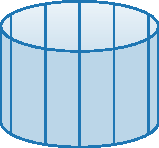
\includegraphics{figures/diagrams/cylinder.pdf}\hspace{1cm}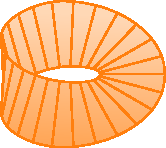
\includegraphics{figures/diagrams/mobius_strip.pdf}\caption{The Möbius strip and te cylinder are both fibre bundles with the same base space (\(\c{S}_1\)) and typical fibre (\([0,1]\)), but different total space and projection.}
\end{figure}

\emphmarginnote{Vector bundles} are fibre bundles where the typical fibre is isomorphic to \(\R^n\). The tangent bundle we have just constructed is the most important example of a vector bundle over a manifold, with total space the tangent bundle, base space the manifold, the natural projection, and typical fibre \(\R^n\). There are other important ones we can construct too. In constructing these, it will be useful to have a version of the \cref{lem:smooth_chart} that is a bit more specialised.
\begin{lemma}[Vector bundle chart lemma]
    Let \(X\) be a smooth manifold (with boundary), and suppose that for each \(p\in X\) we have \(E_p\), a \(k\)- dimension vector space. Let \(E = \coprod_{p\in X} E_p\), and \(\pi: E\to X\) be the map such that \(\pi: E_p \mapsto p\). If have the following:
    \begin{enumerate}[noitemsep]
        \item an open cover of \(X\), \(\cbr{U_a}_{a\in A}\).
        \item for each \(a \in A\), a bijection \(\Phi: \pi^{-1}(U_a) \to U_a \times \R^k\).
        \item for each \(a, b\in A\) with \(U_a \^ U_b \neq \emptyset\), a smooth map \(\tau_{ab} U_a\^ U_b \to \groupGL[k, \R]\) such that the map \(\Phi_a\circ \Phi_b^{-1}: (U_a\^ U_b) \times \R^k \to (U_a\^ U_b) \times \R^k\) is of the form \[ \Phi_a\circ \Phi_b^{-1}(p, v) = (p, \tau_{ab}(p)v)\]
    \end{enumerate}
    Then E has a unique topology and smooth structure making it into a smooth manifold with or without boundary and a smooth rank-k vector bundle over M; with \(\pi\) as projection and \(\cbr{(U_a, \Phi_a)}\) as smooth local trivializations.
\end{lemma}

Say something about frames?

\subsubsection{Principle bundles}
Another type of bundle that is important in the study of Riemannian manifolds are \emphmarginnote{principle \(G\)-bundles}, where \(G\) is a Lie group. This type of bundle associates the action of the Lie group \(G\) to the fibres of a bundle in a specific way. If \((E, B, \pi, F)\) is a fibre bundle, and we have a right group action \(\rho: P\times G\to P\) such that \begin{enumerate}[noitemsep]
    \item \(\rho\) \emph{preserves the fibres} of the bundle, i.e for \(p\in P\), \(g \in G\), then \(\pi(p) = \pi(\rho(p, g))\).
    \item \(\rho\) acts \emph{freely}, that is for \(g\in G\) and \(p\in P\), \(p\cdot g\neq p\) unless \(g\) is the identity element of \(G\). 
    \item \(\rho\) acts \emph{transitively} on the fibres, i.e. if \(b \in B\), and \(p \in \pi^{-1}(b)\), then the map \(g \mapsto p\cdot g\) is a homeomorphism from the group \(G\) onto the fibre \(\pi^{-1}(b)\).
\end{enumerate}
then the combination of the fibre bundle and \(\rho\) is a principle \(G\)-bundle. This definition is quite abstract, but important concrete examples of this exist. 

The \emphmarginnote{frame bundle} is one such example. For a given \(n\)-dimension vector bundle, \((E, X, \pi, V)\), we can construct a new fibre bundle containing all the possible \emphmarginnote{frames} (an ordered choice of basis) of this vector bundle. At a point \(p\in M\) we can think of a frame as a linear isomorphism between \(\R^n\) and the fibre at \(p\), \(V_p = \pi^{-1}(p)\). From our previous discussion of bases with respect to the change in chart, we saw that all choices of basis are related by an element of the general linear group \(\groupGL\). If we denote the set of all frames at \(p\) as \(F_p\), then we see that the action \(\groupGL\) on this is free and transitive. We then define the frame bundle as the disjoint union of the set of frames at each point, \[F(E) = \disjointU_{p\in X} F_p\]. The \emphmarginnote{topology on the frame bundle} is inherited from the topology on the vector bundle it is associated with, which itself



\subsection{Cotangent bundles and covector fields}

On a manifold, we denote the \emphmarginnote{cotangent space} at \(p\), \(T^*_pX\) to be the dual of the tangent space \[T^*_pX = \del{T_pX}^*\]. Elements of this are called \emphmarginnote{cotangent vectors}.

Given a chart on the manifold, \((U, \phi)\), and the induced basis on the tangent space, \(\cbr{\eval{\partial \phi_i}_p}\), we can define a basis on the cotangent space, \(\cbr{\eval{\d\phi^{i}}_p}\) by \(\eval{\d\phi^i}_p (\eval{\partial \phi_j}_p) = \delta^i_j\). Our choice of notation of \(\eval{\d \phi_i}_p\) will become apparent.

Previously, we saw how under a change of coordinates from \((U, \phi)\) to \((V, \psi)\) the coefficients of a tangent vector \(v\in T_pX\) transformed under the Jacobian of the differential. The coefficients of a cotangent vector also transform under the Jacobian, but in the opposite way. For \(v\in T_pX\), \(v = v^i \eval{\partial\phi_i}_p = \tilde v^i \eval{\partial \psi_i}_p\) and \(\omega \in T^*_pX\), \(\omega = \omega_i \eval{\d\phi_i}_p = \tilde \omega_i \eval{\d\psi_i}_p\) we get the transforms \[\underset{\text{Tangent vector transformation}}{\tilde v^j = \pd{\psi^j}{\phi^i}(p) v^i} \quad \quad \quad \underset{\text{Cotangent vector transformation}}{\omega_i = \pd{\psi^j}{\phi^i}(p)\tilde \omega_j}\]. This transform definition is equivalent to saying that \(\tilde \omega_j = \del{\pd{\psi^j}{\phi^i}(p)}^{-1} \omega_i\). Plugging this into the definition of the cotangent vectors and working it through in coordinates, we see that this leave the action of the cotangent vector on the tangent vector in coordinates invariant to the choice of coordinates, as we would expect.

Identically to the tangent bundle we can build the \emphmarginnote{cotangent bundle} from cotangent spaces, and this too is a \(2n\)-dimension manifold and a vector bundle. We build the natural coordinates again out of the bases induced by charts. Sections of this are called \emphmarginnote{covector fields}, denoted \(\omega \in \Gamma(T^*X)\). They are \emph{also} know as \emphmarginnote{differential 1-forms}, and the reason for this will again be apparent later. We can also break a covector field into component functions. The action of a covector field \(\omega \in \Gamma{T^*X}\) on a vector field \(V \in \Gamma(TX)\) is defined by \[\omega(V): X \to \R, \quad\quad \omega(V)(p) = \omega_p(V_p)\].

\todo{discuss coframes?}

\subsection{The differential of smooth functions}

The \emphmarginnote{gradient} of a function of a smooth function \(f: \R^n \to \R\) is one of the objects of central study in calculus. In this setting, it is equal to \[\Grad f = \sum_{i=1}^n \pd{f}{x^i} \pd{}{x^i}\]. In the absence of coordinates, this definition no longer makes sense.

We can associate the portal derivatives of smooth function to components of a vector field. However, it turns out to be more natural to associate them with covector fields. We specify the coordinate free definition of the \emphmarginnote{differential of a smooth function on a manifold} by its action on a tangent vector. \[\d f_p(v) = vf \quad f\in C^\infty(X), \; v \in T_pX\]. This definition of the differential maps smooth functions to \emph{smooth covector fields}\marginnote{\cite[proposition 11.18]{lee2013smooth}}.

Computing the effect of the differential in a chart, we see that \[\d f_p(\eval{\partial \phi^i}_p) = \pd{f}{\phi^i}(p)\]. This gives us the coordinate representation \[\d f_p = \pd{f}{\phi^i}\d \eval{\phi^i}_p\]. The components functions of this covector field are exactly the partial derivatives of \(f\), and so we see this as the analog to the classical gradient. 

If we apply the differential to one of the component functions of a chart \(\phi_i: U \to \R\) we see that \[\d (\phi_j)(p) = \pd{\phi^j}{\phi^i}(p) \eval{\d\phi^i}_p = \delta_i^j \eval{\d\phi^i}_p = \eval{\d\phi^j}_p\]. So the differential of our i'th component function is exactly the i'th basis element of the cotangent space, motivating our notation.

Like the classical gradient, this satisfies a number of properties. For \(a,b \in \R \; f,g \in \C^\infty(X)\):
\begin{itemize}[noitemsep]
    \item \(\d (af + bg) = a\d f + b \d g\) .
    \item \(\d (fg) = f \d g + g \d f\).
    \item \(\d (f/g) = (g \d f - f \d g) / g^2\) where \(g \neq 0\).
    \item If \(I \subset f(X) \subset \R\) is an interval, and \(h: I \to \R\) is smooth, then \(\d (h \circ f) = (h' \circ f) \d f\).
    \item If \(f\) is constant, then \(\d f = 0\).
\end{itemize}


\subsection{Tensor bundles and tensor fields}

Having discussed tangent and cotangent bundles and their sections, we can also talk about higher-order tensor (see \cref{sec:tensors}) bundles. We can define the \emphmarginnote{tensor bundles over \(X\)}

% \begin{tabular}{lcc}
%     \emphmarginnote{The bundle of covariant \(k\)-tensors on \(X\)} & \(T^kT^*X = T^{(0,k)}\) \\
%     \emphmarginnote{The bundle of contravariant \(k\)-tensors on \(X\)} & \(T^kTX = T^{(k, 0)}\) \\
%     \emphmarginnote{The bundle of mixed \((k,l)\)-tensors on \(X\)} & \(T^{(k,l)}TX\) \\
% \end{tabular}



% - manifolds - Manifolds are ways of understanding some complex space by breaking it into sections  %and mapping the sections onto a simpler space. We can use this to "glue" together the sections to get spaces that locally resemble the simple space, but have globally a very different structure. 

% -They are defined by an atlas of charts, that are invertible maps between the simple space and a subset of the manifold, and results in transition maps, that tell you how to map overlapping charts to one another. If the transitions maps (and charts?) preserve a certain structure then you get specific structure preserved on the manifold. The most useful of these preservations 

- Topological manifolds - the charts are continuous wrt to the topology on the simple space / manifolds

- Differentiable manifolds the transition maps have a notion of differentiation and are differentiable up to some degree, \(C^k\), \(k \in \{\N \cup \infty\}\).

\subsection{Tangent space and bundle}
With differentiable manifolds we can introduce the notion of tangent vectors and space as derivatives relating to coordinate charts

\subsection{Generic bundles}
Maybe refer to wieler?

\subsection{Riemannian Manifolds}
adds addition structure that allows us to define distances, along with a host of more complex tools. This is the layer where they become good models of physical surfaces.

\subsubsection{Definition of the metric}
- an inner product in the tangent space

\subsubsection{Geodesics}
- unit speed curves following the metric

\subsubsection{Exponential and Log maps}
- maps between the tangent space and the manifold

\subsection{Manifolds with boundary}

\subsection{Useful examples}
- spheres, toruses, hyperbolic space, polytopes, spd matrices


\section{Lie Groups}
brief section, mostly intro to basic concepts
goal is to get to homogenous spaces / lie groups - maybe put in the prev sections?

Ref risi kondor thesis, weiler, cohen
\subsection{Elementary concepts}
subgroups, stabilisers, products / semidirect products
\subsection{Homogenous spaces}
quotients of groups by a stabaliser - useful as you get an action on the homogenous space

\subsection{Lie groups}
Groups that are manifolds

\subsection{Useful examples}
SO, SE, E, O, SPD, GL

% Groups are very basic mathematical objects that are a building block for much of modern mathematics. A group consists of two elements, a set \(G\) and a operation \(\cdot : G \times G \to G \) that satisfies certain axioms. 
% \begin{definition}[Groups]
%     A group it a tuple \((G, \cdot)\), where \(G\) is a set and \(\cdot :G \times G\to G\) is a function satisfying the following group axioms:
%     \begin{enumerate}
%         \item Closure. For and \(g, h \in G\), \(g \cdot h\) is also an element of \(G\).
%         \item Associativity. For and \(g, h, i \in G\), \((g \cdot h) \cdot i = g \cdot (h\cdot i)\).
%         \item Identity. There is a unique element in \(G\), typically labelled \(e\), called the \emph{identity} for which \( g \cdot e = e \cdot g = g\) for any \(g \in G\).
%         \item Inverse. For any \(g\in G\) there exists another element 
%     \end{enumerate}
% \end{definition}

\section{Stochastic differential equations}

\emphmarginnote{Stochastic differential equations} (SDEs) will be the third core technical tool in this thesis. Here I give some preliminaries on the subject for the interested reader. Recc sme books?

\subsection{A review of measure theory based probability}

Something about the need for measure theory

A \emph{\(\sigma\)-algebra}, much like a topology, is a collection of sets obeying a set of rules. The definition even looks very similar. But this is where the similarity ends. 
\begin{definition}[Measurable space]
    A measurable space (\(X, \sigalg{X}\)) is a set \(X\) along with a collection of subsets \(\sigalg{X}\) of \(X\), called a \emphmarginnote{sigma/\(\sigma\)-algebra}, that satisfy the following:
    \begin{itemize}
        \item \(X \in \sigalg{X}\), and is called the \emph{universal set}.
        \item \(\sigalg{X}\) is closed under \emph{compliments}.
        \item \(\sigalg{X}\) is closed under \emph{countable} unions.
    \end{itemize}
\end{definition}
From this it also follows that a \(\sigma\)-algebra is closed under countable intersections, and that \(\emptyset \in \sigalg{X}\). The definition of a \(\sigma\)-algebra may seem rather abstract, but it has a number of nice properties.

Firstly it contains the limits of any sequence of sets contained within it, which allows us to define some sensible concepts of convergence of random variables, discussed later. For this, at a minimum, we need closure under countable unions and intersections. 

For a sequence of sets \(A_1, A_2, ....\) the \emphmarginnote{limit supremum} or outer limit is the set of elements that appear in \emph{infinitely many} of the \(A_n\). The \emphmarginnote{limit infimum} or \emph{inner limit} is the set of elements that appear in \emph{all but finitely many} \(A_i\), \[\limsup_{n\to \infty} A_n = \Int_{n=1}^\infty \U_{m=n}^\infty A_m \quad\quad \liminf_{n\to \infty} A_n = \U_{n=1}^\infty \Int_{m=n}^\infty A_m\]. These are related by a couple of simple identities \[ \liminf_{n\to \infty} A_n \subseteq \limsup_{n\to\infty}A_n \quad \del{\liminf_{n\to \infty} A_n}^c = \limsup_{n\to \infty}A_n^c\]. The \emphmarginnote{limit of a sequence of sets} is defined if and only if the limit supremum and limit infimum agree, i.e. \[\liminf_{n\to \infty} A_n = \limsup_{n\to\infty}A_n \implies \lim_{n\to \infty}A_n = \liminf_{n\to \infty} A_n = \limsup_{n\to\infty}A_n\]

needed to get to the point. ref some better intro material

- pushforward measures 
- also in one argument 
- conditional probabilities
- what is a density
% In order to work with probability on more complex spaces we require the language of measure theory and its application to probability. Here I give a brief review of the basic definitions of measure theory.

% In order to define probabilities on some space, that space must be a \emphmarginnote{measurable space}. A measurable space is a tuple \((X, \c{X})\) consisting of a a set \(Y\) and a \parmarginnote{\(\sigma\)-algebra} \(\c{X}\). The \(\sigma\)-algebra \(\c{X}\) is a set of subsets of of \(X\) that one can "measure". The \(\sigma\)-algebra must satisfy a set of axioms. These are that is must be closed under \emph{countable} intersections and unions, compliments. A useful corollary of this is that the \(\sigma\)-algebra also contains the limits of \emph{monotone sequences} of sets. In terms of probability, and thinking about each element of the set as a possible event, these are the sets of events we can ask probabilistic questions about.

\subsubsection{Sigma algebras and topologies on product spaces}
The interaction of \(\sigma\)-algebras and topologies on product spaces is one that requires an amount of subtly. 

% As with topologies, creating \(\sigma\)-algebras on product spaces is a necessity.
% First let us consider finite products on a collection of measurable spaces, \((X_a, \sigalg{X_a})_{a\in A}\).

% The \emphmarginnote{product \(\sigma\)-algebra} is generated by the collection of sets \[\cbrcolon{S_i \times ... \times S_n}{S_a \in \sigalg{X_a}, a\in A}\]. The \emphmarginnote{cylinder \(\sigma\)-algebra} is generated by the collection of sets \[\cbrcolon{\pi^{-1}_a(S_a)}{S_a \in \sigalg{X_a}, a \in A}\].We can see that the set \(\pi^{-1}_a(S_a) = S_a \prod_{a\in A\takeaway\cbr{a}}\)


\subsection{Stochastic processes}

Let \(\del{\Omega, \c{F}, \P}\) be a probability space, \(\del{S, \sigalg{S}}\) be a measurable space, called the \emph{observation space}, and \((I, \sigalg{I})\) a measurable, called the \emph{index set}.

A \emphmarginnote{stochastic process} is a function \(X: \Omega\x I \to S\) that is measurable from \(\c{F}\otimes\sigalg{I}\) to \(\sigalg{S}\). The index set and observation space can really be any measurable space that we like, but the usual study of stochastic processes is limited to some specific cases.

Typically the observation space is Euclidean space of some dimension, \(S=\R^n\). We will begin with this, and then later study the case where \(S=X\), a Riemannian manifold. The stochastic process can even take values in more abstract spaces, such as the tangent space at a point on a manifold.

In the simple case, the index set could be a finite collection of indices, \(1, ..., n\), or a countable number of points \(1, 2, ...\) with the discrete \(\sigma\)-algebra. Random variable over \(\R\), and multivariate distributions fall into these camps. These are not the interesting cases for stochastic process however. More interesting is when the index set is uncountable, and comes with some additional structural information, such as a topology or a metric. The index set \(I\) is often chose to be time and can be \(\cobr{0, \infty}\) or \(\sbr{0,T}\), but can also be other spaces such as Riemannian manifolds or other metric spaces. For now, we will use time, \(t \in \cobr{0, \infty}\) or  \(t \in \sbr{0,T}\) as our index set. This index set is both a metric space, and so has a topology, and is also \emph{totally ordered}.

By fixing the index argument this can be thought of as an indexed collection of random variables \(\cbrcolon{X_i: \Omega \to S = X(\cdot, i)}{i\in I}\). By fixing the \(\omega\) argument, we can can think of the \emphmarginnote{sample paths} of \(X\) as the functions \(X(\omega, \cdot): I \to S\). From this point of view we can see a stochastic process as a \emph{function-valued} random variable.

The \emphmarginnote{law of a stochastic process} is defined as \(\mu = \P \circ X^{-1} = X_* \P\), the pushforward measure in the first argument. The \emphmarginnote{finite-dimension marginals} of a stochastic process are the pushforwards of the projection of the law onto a finite index set. For \(\c{I}(i_1, ..., i_k) \subset I\), \(\mu_{i_1, ..., i_k} = (\proj_\c{I})_*\mu\). This is equivalent to saying \(\mu_{i_1, ..., i_k}(F_1\x ...\x F_k) = \P\sbr{\cbrcolon{\omega}{X(\omega, i_1)\in F_1, ..., X(\omega, i_1)\in F_n}}\).

One of the most important theorems in the study of stochastic processes is the \emph{Kolmogorov extension theorem}. Opposite to the projection discussed above, it tells us that if we can write down all sets of finite-dimension marginals, and they agree properly, then the overall stochastic process exists. There exist many statements of this theorem, often with specific index sets or observation space. A more generic statement for topological spaces is
\begin{theorem}[Kolmanagorov Extentsion Theorem]
    Let \(\del{\del{X_a, \sigalg{X_a}}, \topo{X_a}}_{a\in A}\) be a arbitrary collection of measurable spaces \(\del{X_a, \sigalg{X_a}}\) each equipped with topology \(\topo{X_a}\). For each finite \(B \subset A\), let \(\mu_B\) be an inner regular probability measure on the sigma algebra \(\sigalg{X_B} = \prod_{a \in B} \sigalg{X_a}\) with the product topology \(\topo{X_B} = \prod_{a\in B} \topo{X_a}\). Let \(C \subset B\). If for all \(C, B\), the measures are compatible in the sense that \[(\pi_{C \leftarrow B})_* \mu_B = \mu_C\], then there exists a unique probability measure \(\mu_A\) on \(\sigalg{X_A}\) such that \[(\pi_B)_* \mu_A = \mu_B\] for all finite \(B \subset A\).
\end{theorem}
\begin{proof}
    \textcite[theorem 2.4.3]{tao11}
\end{proof}
\todo{Kolmonogorov contiuity thm}
The above generally does not uniquely specify an SP though. There is a lot of "wiggle room" in the choice of \(X_t\) that still matches the right marginals and law. We can under conditions however choose one that is continuous a.s. using the KCT. Find a more general statement? Have one for complete metric spaces. 

An important class of stochastic process if that of \emph{martingales}. In order to define this, we need the concept of a \emph{filtration}. A \emphmarginnote{filtration} on a sigma algebra \(\sigalg{}\) is a collection of sigma algebras indexed by a totally ordered set \(\cbr{\sigalg{i}}_{i \in I}\), such that for all \(0 \leq i < j\), \[\sigalg{i} \subset \sigalg{j} \subset \sigalg{}\]. A stochastic process \(X_t\) on the probability space \((\Omega, \c{F}, \P)\) is a \emphmarginnote{martingale} with respect to the filtration \(\mathbb{F} = \cbr{\c{F}_t}_{t\in \ocbr{0, \infty}}\) if 
\begin{enumerate}[noitemsep]
    \item \(X_t\) is \(\c{F}_f\)-measurable for all \(t\).
    \item \(\E\sbr{\norm{X_t}_2} < \infty\) for all \(t\).
    \item \(\E\sbr{X_s \given \c{F}_t} = X_t\) for all \(s \geq t\).
\end{enumerate}
Effectively this says that the distribution of the  process 1. at time \(t\) is only dependant on its "history" (times \( < t\)), not its "future" (times \( > t\)), 2. that it is integrable, and 3. that the best guess for the process into the future is the last observed value.

The central martingales studied is that of the Brownian motion. Later we will see this arises in a number of different ways, and can be generalised greatly, but for now, we can specify the \emphmarginnote{Brownian motion on \(\R^n\)} via its finite dimension marginals. Let \[p(t, \v{x}_1, \v{x}_2) = \frac{1}{{2\pi t}^{n/2}} e^{-\frac{\norm{\v{x}_1 - \v{x}_2}^2_2}{2t}} \quad \text{for } \v{x}_1, \v{x}_2 \in \R^n, \; t>0\]. For \(0 \leq t_1 \leq ... \leq t_k\) we define the finite dimension marginal \(\nu_{t_1, ..., t_k}\) by picking some \(\v{x}\) to start the Brownian motion at and setting \[\nu_{t_1, ..., t_k}(F_1, ..., F_k) = \int_{F_1, ..., F_k} p(t_1, \v{x}, \v{x}_1)p(t_2-t_1, \v{x}_1, \v{x}_2) ... p(t_k-t_{k-1}, \v{x}_{k-1}, \v{x}_k) \d \v{x}_1...\d \v{x}_n \]. We use the convention that \(p(0, \v{x}_1, \v{x}_2) = \delta_{\v{x}_1}(\v{x}_2)\), and that \(\d \v{x}_1...\d \v{x}_n\) is the Lebesgue measure on \(\R^{n^k}\). 

This satisfies the conditions of Kolmonogorov's extension theorem, giving us a stochastic process, \(B_t\), with these marginals, and with law we denote \(\P^{\v{x}}\) such that \[\P^{\v{x}} (B_{t_1} \in F_1, ..., B_{t_k}\in F_k) = \nu_{t_1,...,t_k}(F_1, ..., F_k)\]. There remains however an ambiguity\todo{explain why}. There exist multiple \(B_t, \P^{\v{x}}\) that satisfy this. 

This leaves us with a choice of which Brownian motion to pick, and we can make it to suit our needs. We do however typically make a canonical choice. This Brownian motion also satisfies the Kolmogorov continuity theorem, so we can chose \(B_t\) such that its paths are continuous almost surely. This ends up being useful as the measure is then defined on the space \(C(\cobr{0, \infty}, \R^n)\) since this space has the structure of a \emphmarginnote{Polish space} (a complete separable metric space), useful properties for analysis. 


\subsection{Differential equations}

Differential equations are a wide class of equations that relate an unknown function to its derivatives.

\emphmarginnote{Ordinary differential equations (ODEs)} are equations of a function of a single variable, \(f(x)\), and its derivatives, \(\od[n]{f}{x}\).

\emphmarginnote{Partial differential equations (PDEs)} are equations of a function of multiple variables, \(f(x_1, ... x_n)\), and its various partial derivatives \(\frac{\partial^{i_1+...+i_n}{f}}{\partial{x^1}^{i_1}...\partial{x_n}^{i_n}}\). 


\emphmarginnote{Linear differential equation} are differential equations that are linear combinations of derivatives, with coefficients that are differentiable functions \(x_1, ..., x_n\).

The \emphmarginnote{order of a differential equation} is the highest order derivative that appears in the equation.

Finding solutions to differential equations is often difficult or impossible analytically, although for a larger class of equations solutions can be found via numerical integration.

One of the more simple differential equations can be written as \[\od{f(t)}{t} = b(t, f(t))\], with \(f: \R \to \R^n\). This is a \emph{first order, non-linear} differential equation. Coupled with an initial point \((f(t_0) = f_0)\), this constitutes an \emphmarginnote{initial value problem}. By the \emphmarginnote{Picard–Lindelöf theorem}, also known as the \emph{Cauchy–Lipschitz theorem}, this has a unique solution, defined by the integral equation \[f(t) = f(t_0) + \int_{t_0}^t b(s, f(t)) \d s\]. If we are lucky, the integral may be analytic. More likely we will need to use numerical solvers to approximate the solution to this equation. In a small abuse of notation, this ODE is typically written as \[\d f(t) = b(t, f(t))\d t\]. From now on we will also replace \(f(t)\) with \(X_t\) to denote the path through a space \(X\) over time. 

The study of stochastic differential equations aims to make rigorous the modification of this differential with the addition of a "noise" term. I.e. how can we make the equation \[\od{X_t}{t} = b(t, X_t) + \sigma(t, X_t) \cdot \text{"noise"}\] rigorous, and how can we integrate this to give us solutions so that the integration \[ X_t = X_0 + \int_0^t b(t, X_t) \d t + \int_0^t \sigma(t, X_t) \cdot "\text{noise}" \d t\] makes sense. 

A stochastic process seems the natural notion to use for the "noise", so let us denote this \(\del{W_t}_{t\geq 0}\). A natural set of conditions for this might be that 
\begin{itemize}
    \item \(W_{t_1} \indep W_{t_2}\) for \(t_1 \neq t_2\).
    \item \(W_t\) is \emph{stationary}, i.e. the distribution of the marginals \(W_{t+t_1}, ..., W_{t+t_n}\) does not depend on \(t\).
    \item \(\E\sbr{W_t}=0\).
\end{itemize}
However it turns out there is no stochastic process that satisfies the first two conditions and has continuous paths. If we add another condition, that the process have unit variance, \(\E\sbr{W_t} = 1\), then the function \((\omega, t) \to W_t(\omega)\) cannot even be measurable with respect to joint sigma algebra \(\c{F} \otimes \sigalg{I}\) to \(\sigalg{S}\) \cite[p. 180]{Kallianpur1980}. It is \emph{possible} to construct a \emphmarginnote{white noise process} satisfying these conditions, however it is defined on a very different, larger space of \emph{generalized functions}, a space where notions such as the Dirac delta can be made rigorous.

\subsection{A reminder on Riemann-Stieltjes integral}

The Riemann-Stieltjes integral is one of a number of useful theories of integration. It is a generalisation of the Riemannian integral that fixes a number of issues. While not as general as Lebesgue or Lebesgue-Stieltjes integration, the analogy of Riemann sums is useful when trying to define stochastic integrals.

The \emphmarginnote{Riemann-Stieltjes integral} of a function \(f: \sbr{a, b}\subset \R \to \R\) with respect to another function \(g: \R \to \R\) is denoted by \[\int_a^b f(x)\d g(x)\]. Given a \emphmarginnote{partition} \(P\) of the interval \(\sbr{a, b}\), we approximate the integral with a summation by \[S(P, f, g) = \sum_{i=0}^{n-1} f(c_i)[g(x_{i+1}) - g(x_i)]\], where \(c_i \in \sbr{x_i, x_{i+1}}\). The \emphmarginnote{norm of a partition} (or mesh) is the length of the largest subinterval, \(\max_i x_{i+1} - x_i\). To define the integral, define a sequence of partitions such that \(\lim_{n\to \infty} \norm{P_n} \to 0\). The the Riemann-Stieltjes integral is defined as \[\int_a^b f(x)\d g(x) = \lim_{n\to\infty} S(P_n, f, g)\], where this converges for all choices of \(c_i \in \sbr{x_i, x_{i+1}}\) and for all sequences of partitions with norm converging to \(0\). 

The class of integrands \(f\) and integrators \(g\) that are integrable is not simple, but for example if \(g\) is of bounded variation (on \(\sbr{a, b}\)), then all continuous functions \(f\) are integrable. One can also under conditions integrate discontinuous functions, but we run into significant issues when \(f\) and \(g\) share discontinuities. 

\subsection{The Ito and Stratonovich integrals}

To define a stochastic integral, we follow a similar process to the Riemann-Stieltjes integral. First we need to choose something to be our noise which we can integrate against. Consider a discretisation of the stochastic process \(X_t\) as \[X_{{k+1}} - X_{k} = b(t_k, X_{k}) \Delta t_k + \sigma(t_k, X_{k}) \text{"noise"} \Delta t_k\] on a partition \(0=t_0 < ... < t_n = t\), \(X_k = X_{t_k}, \; W_k = W_{t_k}, \; \Delta t_k = t_{k+1} - t_k\). Lets replace \(\text{"noise"} \Delta t_k\) with \(\Delta V_k = V_{t_{k+1}} - V_{t_k}\), the difference between some timepoints of a stochastic process \(\del{V_t}_{t \geq 0}\), a this seems a reasonable choice for the noise.

If we review our previous conditions for the "noise" term (stationary, independent, mean \(0\)) and instead apply them to the \emph{increments} \(\Delta V_{k}\), it turns out that only one stochastic process that satisfies these conditions, and it is the Brownian motion. Later we will see that we can integrate against a wide class of stochastic processes, but for now we will focus on integrating again Brownian motion. Thus, we approximate our stochastic differential equation by \[X_k = X_0 + \sum_{j=0}^{k-1} b(t_j, X_{j}) \Delta t_j + \sum_{j=0}^{k-1} \sigma(t_j, X_{j}) \Delta B_j \], giving rise to and integral of the form \[X_t = X_0 + \int_0^t b(s, X_x) \d s + "\int_0^t \sigma(s, X_s) \d B_s"\]. The first term is the Riemann-Stieltjes integral, but the second is new, and we will need to see find a way to define this integral.

For a sequence of partitions \(P_n\) such that \(\lim_{n\to \infty}\norm{P_n} \to 0\), define \[S(P_n, f, \del{B_t}_{t \geq 0}, \omega) = \sum_{i=0}^{n-1} f(c_i, \omega)\sbr{B_{t_{i+1}} - B_{t_i}}(\omega)\], again with \(c_i\in \sbr{t_i, t_{i+1}}\), and then define the integral as \[\int_0^t f(s, \omega) \d B_s(\omega) = \lim_{n\to \infty} S(P_n, f, \del{B_t}_{t \geq 0}, \omega)\]. As it turns out, this is not very well behaved with respect to the choice of \(c_i\), unsurprising as although we can choose the paths of our Brownian motion to be continuous, it is nowhere differentiable, and the total variation of the paths is in fact infinite almost surely, making it very poorly behaved as a Riemann-Stieltjes integral.

As an example of this, let us look at the example where we choose \(f(t, \omega) = B_t(\omega)\), and choose \(c_i = t_i + \alpha(t_{i+1} - t_i)\), where \(\alpha\) interpolates between choosing the start and end of the intervals in the discretisation. Then \[\E\sbr{S(P_n, f, \del{B_t}_{t \geq 0}, \omega)} &= \E\sbr{\sum_{i=0}^{n-1} f(c_i, \omega)\sbr{B_{t_{i+1}} - B_{t_i}}(\omega)} \\ &= \sum_{i=0}^{n-1} \E\sbr{B_{t_i + \alpha\del{t_{i+1} - t_i}}(\omega)\sbr{B_{t_{i+1}} - B_{t_i}}(\omega)} \\ &= \sum_{i=0}^{n-1} \E\sbr{{\sbr{B_{t_i + \alpha\del{t_{i+1} - t_i}} - B_{t_i}}(\omega)}^2} \\ &= \alpha t \]. Seeing as this is independent of the discretisation, we see that the choice of \(\alpha\) affects greatly the value the integral converges to. Nonetheless, we can develop a coherent theory of integration for stochastic integrals by fixing an \(\alpha\) and working through the consequences. There is much debate in the literature as to whether this choice of \(\alpha\) is philosophically important, or if it is simply a modelling assumption. While theory exists for \(\alpha\in\sbr{0,1}\), the two choices that prove most useful are \emphmarginnote{The \ito~integral}, \(\alpha=0\), usually denoted by \[\int_a^b f(t, \omega) \d B_t(\omega)\], along with the abuse of notation differential equation form \[\d X_t = \sigma(t, X_t) \d B_t\] and \emphmarginnote{the Stratonovich integral}, \(\alpha= \frac{1}{2}\), usually denoted \[\int_a^b f(t, \omega) \circ \d B_t(\omega)\], along with the abuse of notation differential equation form \[\d X_t = \sigma(t, \omega) \circ \d B_t\]. For \(\alpha \in \sbr{0,1}\) I will use \(\circ_\alpha\).

Briefly, what type of functions \(f(t, \omega)\) can we integrate, and what can we integrate them against? It can be shown that these integrals can be defined (i.e. the Riemann sums converge in probability on \(L^2\) in the limit) for any integrator \(\del{W_t}_{t\geq 0}\) the is a \emph{semimartingale}. A \emphmarginnote{semimartingale} is a stochastic process the can be decomposed into two more stochastic processes, \(W_t = M_t + A_t\), where \(M_t\) is a \emphmarginnote{local martingale}, a relaxed, localised version of the martingale property \todo{see ...}, and \(A_t\) is a stochastic process with bounded total variation. Against this integrator we can integrate any stochastic process \(\del{H_t}_{t\geq0}\) that has left-continuous \todo{cadlag?}, locally bounded paths that is adapted to \(W_t\). 

\subsubsection{Advantages to different stochastic integrals}\todo{alpha type?}
How then should be choose the value of \(\alpha\) to use? Both choices of \(\alpha\) have advantages and disadvantages. The \ito~integral primarily is attractive as function evaluations, \(f(c_i, \omega)\), are independent of the Brownian motion increments, \(\sbr{B_{t_{i+1}} - B_{t_i}}\). Firstly, this is attractive in definition as the process doesn't "look ahead" to evaluate the integrand. Secondly, if we look at \emphmarginnote{\ito{} processes}, processes which can be written as \[X_t = X_0 + \int_0^t b(s, \omega) \d s + \int_0^t \sigma(s, \omega) \d B_t\], leads to the fact that \(\E\sbr{\int_0^t f(t, \omega) \d B_t} = 0\) and the \emphmarginnote{martingale representation theorem}, which gives the connection that \[X_t \text{ is a martingale} \iff X_t \text{ is an \ito~process}\]. This property is very useful mathematically and makes proving statements about \ito integrals much easier. On the other hand, the \ito integral behaves poorly with a change of variable. \emphmarginnote{\ito's formula} states that for a twice differentiable function \(g(t, X_t) \in C^2\del{\cobr{0, \infty}, \R}\), the \ito{} process \(Y_t = g(t, X_t)\) is given by the formula \[\d Y_t &= \sbr{\pd{g}{t}(t, X_t) + \frac{1}{2} \pd[2]{g}{x}(t, X_t) \sigma(t, X_t)}\d t + \pd{g}{x}(t, X_t) \d X_t \\ &= \sbr{\pd{g}{t}(t, X_t) + \frac{1}{2} \pd[2]{g}{x}(t, X_t) \sigma(t, X_t) + \pd{g}{x}(t, X_t) b(t, X_t) }\d t + \pd{g}{x}(t, X_t) \sigma(t, X_t) \d X_t\]. Where we see an extra term involving the second derivative appears. This can make working with changes of variable trickier.

Ths Stratonovich integral, even against Brownian motion, are in general \emph{not} martingales. They also "look into the future" in the sense that the evaluation of the integrand in the discretised intervals is statistically dependent on the value of the jump of the integrator. It instead has a different intuitive interpretation. If we define a series of stochastic processes, \(\del{B_t^\tau}_{t \geq0}\), that converge to the white noise process in the limit \(\tau \to 0\), for example a Gaussian process with kernel \(\Sigma_{ij} = \exp\sbr{\frac{-(t_I - t_j)^2}{\tau^2}}\), and we define a series of stochastic differential equations as \[\od{X_t^\tau}{t} = b(t, X_t^\tau) + \sigma(t, X_t^\tau) \od{B_t^\tau}{t}\], the the solutions to this series of differential equations converges to the solution to the Stratonovich differential equation \[\d X_t = b(t, X_t)\d t + \sigma(t, X_t) \circ \d B_t\]. The \emphmarginnote{change of variable formula for Stratonovich integrals} is much nicer to work with. For a for a twice differentiable function \(g(t, X_t) \in C^2\del{\cobr{0, \infty}, \R}\), the \ito{} process \(Y_t = g(t, X_t)\) is given by the formula \[\d Y_t &= \pd{g}{t}(t, X_t)\d t + \pd{g}{x}(t, X_t) \d X_t \\ &= \sbr{\pd{g}{t}(t, X_t)  + \pd{g}{x}(t, X_t) b(t, X_t) }\d t + \pd{g}{x}(t, X_t) \sigma(t, X_t) \d X_t\].\todo{check?}

\subsubsection{Connections between different stochastic integrals}
From a technical and philosophical point of view, it is useful that there is a strong connection between integrals defined with \(\alpha\in \sbr{0,1}\). For a stochastic differential equation of the form \[\d X_t = b(t, X_t) \d t + \sigma(t, X_t) \circ_\alpha \d B_t\], with solution \(\del{X_t}_{t \geq 0}\) given by \[ X_t = X_0 + \int_0^t b(s, X_s) \d s + \int_0^t \sigma(s, X_s) \circ_\alpha \d B_s\] then \(X_t\) is also the solution to a \emph{modified \ito~equation} \[\d X_t = \sbr{b(t, X_t) + \alpha \pd{\sigma}{t}(s, X_s)\sigma(s, X_t)} \d t + \sigma(t, X_t) \d B_t\] with solutions given by \[X_t = X_0 = \int_0^t b(s, X_s) + \alpha \pd{\sigma}{t}(s, X_s)\sigma(s, X_t) \d s + \int_0^t \sigma(s, X_s) \d B_s\]. Using this connection we can map between using any \(\alpha\) we desire, particularly between the \ito{} and Stratonovich forms for the technical properties.

\todo{When do they coincide? When sigma is spatial constant. When sigma is continuous. When sigma varys smoothly in the sense from oskendel 3.10}

\subsubsection{Multidimension stochastic differential equations}

\subsubsection{Solutions to stochastic differential equations}

An important question to ask is when a stochastic differential equation that we write down has a solution, and when these solutions are unique. This can be summarised neatly for Euclidean stochastic differential equations via the following theorem
\begin{theorem}[Existance and uniqueness of solutions to a stochastic differential equation]
    Let \(T >0\) and 
    \begin{itemize}[noitemsep]
        \item \(b: \sbr{0, T} \times \R^n \to \R^n\)
        \item \(\sigma: \sbr{0, T} \x \R^n \to \R^{n \times m}\)
    \end{itemize} be measurable functions satisfying \[\norm{b(t, x)}_2 + \norm{\sigma(t, x)}_2 \leq  C(1 + \norm{x}_2), \quad x\in\R^n, t\in\sbr{0,T} \label{eq:exist_unique_cond_1}\] for some constant \(C\), and \[\norm{b(t, x) - b(t, y)}_2 + \norm{\sigma(t, x) - \sigma\del{t, y}}_2 \leq D\norm{x-y}_2 \label{eq:exist_unique_cond_2}\] for some constant \(D\). Let \(\c{F}_\infty\) be the \(\sigma\)-algebra generated by the \(m\)-dimension Brownian motion \(\del{B_t}_{t\geq 0}\), and \(Z\) be a random variable independent of this \(\sigma\)-algebra such that \(\E\sbr{\norm{Z}_2^2} < \infty\).

    The the stochastic differential equation \[\d X_t = b(t, X_t) \d t + \sigma(t, X_t) \d B_t, \quad 0\leq t\leq T, \; X_0 \sim Z\] has a unique \(t\)-path-continuous solution \(X_t(\omega)\) such that at tie \(t\), \(X_t(\omega)\) is adapted to the filtration \(\c{F}_t^Z\) generated by \(Z\) and \(\del{B_s}_{s\leq t}\). In addition \[\E\sbr{\int_0^T \norm{X_t}_2^2 \d t} < \infty .\]
\end{theorem}\begin{proof}
    \textcite[p. 66]{oksendal2003stochastic}
\end{proof}. The conditions of this theorem are reasonably natural. Condition \ref{eq:exist_unique_cond_1} tells us that the coefficients of the process do not blow up too fast, and so the process does not explode, i.e. that \(\norm{X_t}_2 < \infty\) for finite time. Condition \ref{eq:exist_unique_cond_2}, effectively a joint Lipschitz condition, says that the coefficients don't change too rapidly, and guarantees the the solutions to the stochastic differential equation is unique, in the sense that if \(X_1(t, \omega)\) and \(X_2(t, \omega)\) are two solutions to the stochastic differential equation, then \[X_1(t, \omega) = X_2(t, \omega)\quad \text{for all } 0 \leq t \leq T, \; \as \]

\subsubsection{Weak solutions}

\todo{uuuhhhh}

\subsection{\ito{} diffusions}

\subsection{Langevin Dynamics}

state some clear Langevin dynamics as I have found them difficult to find, and discuss implications of these (sgld, langevin sampling etc)

\subsection{Girsanov theory}

Give a brief account of what this type of tho does and why its important. 

\subsection{Time-reversal results}

Give a brief account of existing results - probably Anderson, Cattieux

\subsection{Stochastic calculus on manifolds}
Worth doing?

\section{Score-matching}
Worth a section to introduce it as an independent concept?

\subsection{ISM}

+ sliced

\subsection{DSM}


\section{Generative modelling}
Possibly now switch this section to just diffusion models? Unless an overview of the others is good to highlight the benefits?
% \begin{figure}[h]
%     \documentclass[tikz,10pt]{standalone}
\usepackage[standalone,commands]{../../MJH}

\graphicspath{/home/mhutchin/GoogleDrive/University - Postgraduate/Theses/Final/figures/diagrams/}

% \usepackage{tikz}
% \usetikzlibrary{positioning}

\usepackage{pgfplots}
\pgfplotsset{compat=1.17}
% \usepgfplotslibrary{external}
% \usepgfplotslibrary{groupplots}
% \usepgfplotslibrary{fillbetween}
% \usetikzlibrary{fadings}

\begin{document}
    % \tikzsetnextfilename{generative_model}
    \begin{tikzpicture}
        \node (simple) {
\includegraphics{../diagrams/simple_distribution.pdf}};
        % \node (simple) {% This file was created with tikzplotlib v0.10.1.
\begin{tikzpicture}

\definecolor{darkcyan23100171}{RGB}{23,100,171}
\definecolor{darkgray176}{RGB}{176,176,176}
\definecolor{ghostwhite247251255}{RGB}{247,251,255}
\definecolor{lavender207225242}{RGB}{207,225,242}
\definecolor{midnightblue848107}{RGB}{8,48,107}
\definecolor{skyblue147196222}{RGB}{147,196,222}
\definecolor{steelblue74151201}{RGB}{74,151,201}

\begin{axis}[
hide x axis,
hide y axis,
tick align=outside,
tick pos=left,
x grid style={darkgray176},
xmin=-2, xmax=2,
xtick style={color=black},
xtick={-2,0,2},
xticklabels={
  \(\displaystyle {\ensuremath{-}2}\),
  \(\displaystyle {0}\),
  \(\displaystyle {2}\)
},
y grid style={darkgray176},
ymin=-2, ymax=2,
ytick style={color=black},
ytick={-2,0,2},
yticklabels={
  \(\displaystyle {\ensuremath{-}2}\),
  \(\displaystyle {0}\),
  \(\displaystyle {2}\)
}
]
\addplot [draw=none]
table{%
x  y
-1.95959595959596 -2
-1.91919191919192 -2
-1.87878787878788 -2
-1.83838383838384 -2
-1.7979797979798 -2
-1.75757575757576 -2
-1.71717171717172 -2
-1.67676767676768 -2
-1.63636363636364 -2
-1.5959595959596 -2
-1.55555555555556 -2
-1.51515151515152 -2
-1.47474747474747 -2
-1.43434343434343 -2
-1.39393939393939 -2
-1.35353535353535 -2
-1.31313131313131 -2
-1.27272727272727 -2
-1.23232323232323 -2
-1.19191919191919 -2
-1.15151515151515 -2
-1.11111111111111 -2
-1.07070707070707 -2
-1.03030303030303 -2
-0.98989898989899 -2
-0.949494949494949 -2
-0.909090909090909 -2
-0.868686868686869 -2
-0.828282828282828 -2
-0.787878787878788 -2
-0.747474747474747 -2
-0.707070707070707 -2
-0.666666666666667 -2
-0.626262626262626 -2
-0.585858585858586 -2
-0.545454545454545 -2
-0.505050505050505 -2
-0.464646464646465 -2
-0.424242424242424 -2
-0.383838383838384 -2
-0.343434343434343 -2
-0.303030303030303 -2
-0.262626262626263 -2
-0.222222222222222 -2
-0.181818181818182 -2
-0.141414141414141 -2
-0.101010101010101 -2
-0.0606060606060606 -2
-0.0202020202020201 -2
0.0202020202020203 -2
0.060606060606061 -2
0.101010101010101 -2
0.141414141414141 -2
0.181818181818182 -2
0.222222222222222 -2
0.262626262626263 -2
0.303030303030303 -2
0.343434343434343 -2
0.383838383838384 -2
0.424242424242424 -2
0.464646464646465 -2
0.505050505050505 -2
0.545454545454546 -2
0.585858585858586 -2
0.626262626262626 -2
0.666666666666667 -2
0.707070707070707 -2
0.747474747474748 -2
0.787878787878788 -2
0.828282828282829 -2
0.868686868686869 -2
0.909090909090909 -2
0.94949494949495 -2
0.98989898989899 -2
1.03030303030303 -2
1.07070707070707 -2
1.11111111111111 -2
1.15151515151515 -2
1.19191919191919 -2
1.23232323232323 -2
1.27272727272727 -2
1.31313131313131 -2
1.35353535353535 -2
1.39393939393939 -2
1.43434343434343 -2
1.47474747474747 -2
1.51515151515152 -2
1.55555555555556 -2
1.5959595959596 -2
1.63636363636364 -2
1.67676767676768 -2
1.71717171717172 -2
1.75757575757576 -2
1.7979797979798 -2
1.83838383838384 -2
1.87878787878788 -2
1.91919191919192 -2
1.95959595959596 -2
2 -2
2 -1.95959595959596
2 -1.91919191919192
2 -1.87878787878788
2 -1.83838383838384
2 -1.7979797979798
2 -1.75757575757576
2 -1.71717171717172
2 -1.67676767676768
2 -1.63636363636364
2 -1.5959595959596
2 -1.55555555555556
2 -1.51515151515152
2 -1.47474747474747
2 -1.43434343434343
2 -1.39393939393939
2 -1.35353535353535
2 -1.31313131313131
2 -1.27272727272727
2 -1.23232323232323
2 -1.19191919191919
2 -1.15151515151515
2 -1.11111111111111
2 -1.07070707070707
2 -1.03030303030303
2 -0.98989898989899
2 -0.949494949494949
2 -0.909090909090909
2 -0.868686868686869
2 -0.828282828282828
2 -0.787878787878788
2 -0.747474747474747
2 -0.707070707070707
2 -0.666666666666667
2 -0.626262626262626
2 -0.585858585858586
2 -0.545454545454545
2 -0.505050505050505
2 -0.464646464646465
2 -0.424242424242424
2 -0.383838383838384
2 -0.343434343434343
2 -0.303030303030303
2 -0.262626262626263
2 -0.222222222222222
2 -0.181818181818182
2 -0.141414141414141
2 -0.101010101010101
2 -0.0606060606060606
2 -0.0202020202020201
2 0.0202020202020203
2 0.060606060606061
2 0.101010101010101
2 0.141414141414141
2 0.181818181818182
2 0.222222222222222
2 0.262626262626263
2 0.303030303030303
2 0.343434343434343
2 0.383838383838384
2 0.424242424242424
2 0.464646464646465
2 0.505050505050505
2 0.545454545454546
2 0.585858585858586
2 0.626262626262626
2 0.666666666666667
2 0.707070707070707
2 0.747474747474748
2 0.787878787878788
2 0.828282828282829
2 0.868686868686869
2 0.909090909090909
2 0.94949494949495
2 0.98989898989899
2 1.03030303030303
2 1.07070707070707
2 1.11111111111111
2 1.15151515151515
2 1.19191919191919
2 1.23232323232323
2 1.27272727272727
2 1.31313131313131
2 1.35353535353535
2 1.39393939393939
2 1.43434343434343
2 1.47474747474747
2 1.51515151515152
2 1.55555555555556
2 1.5959595959596
2 1.63636363636364
2 1.67676767676768
2 1.71717171717172
2 1.75757575757576
2 1.7979797979798
2 1.83838383838384
2 1.87878787878788
2 1.91919191919192
2 1.95959595959596
2 2
1.95959595959596 2
1.91919191919192 2
1.87878787878788 2
1.83838383838384 2
1.7979797979798 2
1.75757575757576 2
1.71717171717172 2
1.67676767676768 2
1.63636363636364 2
1.5959595959596 2
1.55555555555556 2
1.51515151515152 2
1.47474747474747 2
1.43434343434343 2
1.39393939393939 2
1.35353535353535 2
1.31313131313131 2
1.27272727272727 2
1.23232323232323 2
1.19191919191919 2
1.15151515151515 2
1.11111111111111 2
1.07070707070707 2
1.03030303030303 2
0.98989898989899 2
0.94949494949495 2
0.909090909090909 2
0.868686868686869 2
0.828282828282829 2
0.787878787878788 2
0.747474747474748 2
0.707070707070707 2
0.666666666666667 2
0.626262626262626 2
0.585858585858586 2
0.545454545454546 2
0.505050505050505 2
0.464646464646465 2
0.424242424242424 2
0.383838383838384 2
0.343434343434343 2
0.303030303030303 2
0.262626262626263 2
0.222222222222222 2
0.181818181818182 2
0.141414141414141 2
0.101010101010101 2
0.060606060606061 2
0.0202020202020203 2
-0.0202020202020201 2
-0.0606060606060606 2
-0.101010101010101 2
-0.141414141414141 2
-0.181818181818182 2
-0.222222222222222 2
-0.262626262626263 2
-0.303030303030303 2
-0.343434343434343 2
-0.383838383838384 2
-0.424242424242424 2
-0.464646464646465 2
-0.505050505050505 2
-0.545454545454545 2
-0.585858585858586 2
-0.626262626262626 2
-0.666666666666667 2
-0.707070707070707 2
-0.747474747474747 2
-0.787878787878788 2
-0.828282828282828 2
-0.868686868686869 2
-0.909090909090909 2
-0.949494949494949 2
-0.98989898989899 2
-1.03030303030303 2
-1.07070707070707 2
-1.11111111111111 2
-1.15151515151515 2
-1.19191919191919 2
-1.23232323232323 2
-1.27272727272727 2
-1.31313131313131 2
-1.35353535353535 2
-1.39393939393939 2
-1.43434343434343 2
-1.47474747474747 2
-1.51515151515152 2
-1.55555555555556 2
-1.5959595959596 2
-1.63636363636364 2
-1.67676767676768 2
-1.71717171717172 2
-1.75757575757576 2
-1.7979797979798 2
-1.83838383838384 2
-1.87878787878788 2
-1.91919191919192 2
-1.95959595959596 2
-2 2
-2 1.95959595959596
-2 1.91919191919192
-2 1.87878787878788
-2 1.83838383838384
-2 1.7979797979798
-2 1.75757575757576
-2 1.71717171717172
-2 1.67676767676768
-2 1.63636363636364
-2 1.5959595959596
-2 1.55555555555556
-2 1.51515151515152
-2 1.47474747474747
-2 1.43434343434343
-2 1.39393939393939
-2 1.35353535353535
-2 1.31313131313131
-2 1.27272727272727
-2 1.23232323232323
-2 1.19191919191919
-2 1.15151515151515
-2 1.11111111111111
-2 1.07070707070707
-2 1.03030303030303
-2 0.98989898989899
-2 0.94949494949495
-2 0.909090909090909
-2 0.868686868686869
-2 0.828282828282829
-2 0.787878787878788
-2 0.747474747474748
-2 0.707070707070707
-2 0.666666666666667
-2 0.626262626262626
-2 0.585858585858586
-2 0.545454545454546
-2 0.505050505050505
-2 0.464646464646465
-2 0.424242424242424
-2 0.383838383838384
-2 0.343434343434343
-2 0.303030303030303
-2 0.262626262626263
-2 0.222222222222222
-2 0.181818181818182
-2 0.141414141414141
-2 0.101010101010101
-2 0.060606060606061
-2 0.0202020202020203
-2 -0.0202020202020201
-2 -0.0606060606060606
-2 -0.101010101010101
-2 -0.141414141414141
-2 -0.181818181818182
-2 -0.222222222222222
-2 -0.262626262626263
-2 -0.303030303030303
-2 -0.343434343434343
-2 -0.383838383838384
-2 -0.424242424242424
-2 -0.464646464646465
-2 -0.505050505050505
-2 -0.545454545454545
-2 -0.585858585858586
-2 -0.626262626262626
-2 -0.666666666666667
-2 -0.707070707070707
-2 -0.747474747474747
-2 -0.787878787878788
-2 -0.828282828282828
-2 -0.868686868686869
-2 -0.909090909090909
-2 -0.949494949494949
-2 -0.98989898989899
-2 -1.03030303030303
-2 -1.07070707070707
-2 -1.11111111111111
-2 -1.15151515151515
-2 -1.19191919191919
-2 -1.23232323232323
-2 -1.27272727272727
-2 -1.31313131313131
-2 -1.35353535353535
-2 -1.39393939393939
-2 -1.43434343434343
-2 -1.47474747474747
-2 -1.51515151515152
-2 -1.55555555555556
-2 -1.5959595959596
-2 -1.63636363636364
-2 -1.67676767676768
-2 -1.71717171717172
-2 -1.75757575757576
-2 -1.7979797979798
-2 -1.83838383838384
-2 -1.87878787878788
-2 -1.91919191919192
-2 -1.95959595959596
-2 -2
-1.95959595959596 -2

-0.324472883686381 -1.91919191919192
-0.343434343434343 -1.9160663051261
-0.383838383838384 -1.90852116670104
-0.424242424242424 -1.90000663184958
-0.464646464646465 -1.89047869403537
-0.505050505050505 -1.87988757491763
-0.508918384395951 -1.87878787878788
-0.545454545454545 -1.8687390284875
-0.585858585858586 -1.85652942463433
-0.626262626262626 -1.84313431096661
-0.639592611261213 -1.83838383838384
-0.666666666666667 -1.8289845436415
-0.707070707070707 -1.81380405924709
-0.745776346953784 -1.7979797979798
-0.747474747474747 -1.79729970941921
-0.787878787878788 -1.78018649540984
-0.828282828282828 -1.76158983483682
-0.836538224711169 -1.75757575757576
-0.868686868686869 -1.74215709080962
-0.909090909090909 -1.72127583341941
-0.916640686161939 -1.71717171717172
-0.949494949494949 -1.69945939855923
-0.988631448111743 -1.67676767676768
-0.98989898989899 -1.67603601551574
-1.03030303030303 -1.651691437786
-1.05418232463594 -1.63636363636364
-1.07070707070707 -1.62574568493161
-1.11111111111111 -1.59828495629982
-1.1144009731905 -1.5959595959596
-1.15151515151515 -1.56955385581596
-1.17018882693894 -1.55555555555556
-1.19191919191919 -1.53909433876947
-1.22205119628112 -1.51515151515152
-1.23232323232323 -1.5068707204197
-1.27047829616178 -1.47474747474747
-1.27272727272727 -1.47281881543358
-1.31313131313131 -1.43691883292068
-1.31593403191767 -1.43434343434343
-1.35353535353535 -1.39894912296432
-1.35868825930117 -1.39393939393939
-1.39393939393939 -1.35868825930117
-1.39894912296432 -1.35353535353535
-1.43434343434343 -1.31593403191767
-1.43691883292068 -1.31313131313131
-1.47281881543358 -1.27272727272727
-1.47474747474747 -1.27047829616178
-1.5068707204197 -1.23232323232323
-1.51515151515152 -1.22205119628112
-1.53909433876947 -1.19191919191919
-1.55555555555556 -1.17018882693894
-1.56955385581596 -1.15151515151515
-1.5959595959596 -1.1144009731905
-1.59828495629982 -1.11111111111111
-1.62574568493161 -1.07070707070707
-1.63636363636364 -1.05418232463594
-1.651691437786 -1.03030303030303
-1.67603601551574 -0.98989898989899
-1.67676767676768 -0.988631448111743
-1.69945939855923 -0.949494949494949
-1.71717171717172 -0.916640686161939
-1.72127583341941 -0.909090909090909
-1.74215709080962 -0.868686868686869
-1.75757575757576 -0.836538224711169
-1.76158983483682 -0.828282828282828
-1.78018649540984 -0.787878787878788
-1.79729970941921 -0.747474747474747
-1.7979797979798 -0.745776346953784
-1.81380405924709 -0.707070707070707
-1.8289845436415 -0.666666666666667
-1.83838383838384 -0.639592611261213
-1.84313431096661 -0.626262626262626
-1.85652942463433 -0.585858585858586
-1.8687390284875 -0.545454545454545
-1.87878787878788 -0.508918384395951
-1.87988757491763 -0.505050505050505
-1.89047869403537 -0.464646464646465
-1.90000663184958 -0.424242424242424
-1.90852116670104 -0.383838383838384
-1.9160663051261 -0.343434343434343
-1.91919191919192 -0.324472883686381
-1.92288337251272 -0.303030303030303
-1.92893268619117 -0.262626262626263
-1.934063075467 -0.222222222222222
-1.9383001797535 -0.181818181818182
-1.94166504980535 -0.141414141414141
-1.94417432210924 -0.101010101010101
-1.94584035604447 -0.0606060606060606
-1.94667133539732 -0.0202020202020201
-1.94667133539732 0.0202020202020203
-1.94584035604447 0.060606060606061
-1.94417432210924 0.101010101010101
-1.94166504980535 0.141414141414141
-1.9383001797535 0.181818181818182
-1.934063075467 0.222222222222222
-1.92893268619117 0.262626262626263
-1.92288337251272 0.303030303030303
-1.91919191919192 0.324472883686381
-1.9160663051261 0.343434343434343
-1.90852116670104 0.383838383838384
-1.90000663184958 0.424242424242424
-1.89047869403537 0.464646464646465
-1.87988757491763 0.505050505050505
-1.87878787878788 0.508918384395952
-1.8687390284875 0.545454545454546
-1.85652942463433 0.585858585858586
-1.84313431096661 0.626262626262626
-1.83838383838384 0.639592611261213
-1.8289845436415 0.666666666666667
-1.81380405924709 0.707070707070707
-1.7979797979798 0.745776346953784
-1.79729970941921 0.747474747474748
-1.78018649540984 0.787878787878788
-1.76158983483682 0.828282828282829
-1.75757575757576 0.836538224711169
-1.74215709080962 0.868686868686869
-1.72127583341941 0.909090909090909
-1.71717171717172 0.916640686161939
-1.69945939855923 0.94949494949495
-1.67676767676768 0.988631448111743
-1.67603601551574 0.98989898989899
-1.651691437786 1.03030303030303
-1.63636363636364 1.05418232463594
-1.62574568493161 1.07070707070707
-1.59828495629982 1.11111111111111
-1.5959595959596 1.1144009731905
-1.56955385581596 1.15151515151515
-1.55555555555556 1.17018882693894
-1.53909433876947 1.19191919191919
-1.51515151515152 1.22205119628112
-1.5068707204197 1.23232323232323
-1.47474747474747 1.27047829616178
-1.47281881543358 1.27272727272727
-1.43691883292068 1.31313131313131
-1.43434343434343 1.31593403191767
-1.39894912296432 1.35353535353535
-1.39393939393939 1.35868825930117
-1.35868825930117 1.39393939393939
-1.35353535353535 1.39894912296432
-1.31593403191767 1.43434343434343
-1.31313131313131 1.43691883292068
-1.27272727272727 1.47281881543358
-1.27047829616178 1.47474747474747
-1.23232323232323 1.5068707204197
-1.22205119628112 1.51515151515152
-1.19191919191919 1.53909433876947
-1.17018882693894 1.55555555555556
-1.15151515151515 1.56955385581596
-1.1144009731905 1.5959595959596
-1.11111111111111 1.59828495629982
-1.07070707070707 1.62574568493161
-1.05418232463594 1.63636363636364
-1.03030303030303 1.651691437786
-0.98989898989899 1.67603601551574
-0.988631448111743 1.67676767676768
-0.949494949494949 1.69945939855923
-0.916640686161938 1.71717171717172
-0.909090909090909 1.72127583341941
-0.868686868686869 1.74215709080962
-0.836538224711168 1.75757575757576
-0.828282828282828 1.76158983483682
-0.787878787878788 1.78018649540984
-0.747474747474747 1.79729970941921
-0.745776346953783 1.7979797979798
-0.707070707070707 1.81380405924709
-0.666666666666667 1.8289845436415
-0.639592611261212 1.83838383838384
-0.626262626262626 1.84313431096661
-0.585858585858586 1.85652942463433
-0.545454545454545 1.8687390284875
-0.508918384395951 1.87878787878788
-0.505050505050505 1.87988757491763
-0.464646464646465 1.89047869403537
-0.424242424242424 1.90000663184958
-0.383838383838384 1.90852116670104
-0.343434343434343 1.9160663051261
-0.324472883686378 1.91919191919192
-0.303030303030303 1.92288337251272
-0.262626262626263 1.92893268619117
-0.222222222222222 1.934063075467
-0.181818181818182 1.9383001797535
-0.141414141414141 1.94166504980535
-0.101010101010101 1.94417432210924
-0.0606060606060606 1.94584035604447
-0.0202020202020201 1.94667133539732
0.0202020202020203 1.94667133539732
0.060606060606061 1.94584035604447
0.101010101010101 1.94417432210924
0.141414141414141 1.94166504980535
0.181818181818182 1.9383001797535
0.222222222222222 1.934063075467
0.262626262626263 1.92893268619117
0.303030303030303 1.92288337251272
0.324472883686378 1.91919191919192
0.343434343434343 1.9160663051261
0.383838383838384 1.90852116670104
0.424242424242424 1.90000663184958
0.464646464646465 1.89047869403537
0.505050505050505 1.87988757491763
0.508918384395952 1.87878787878788
0.545454545454546 1.8687390284875
0.585858585858586 1.85652942463433
0.626262626262626 1.84313431096661
0.639592611261212 1.83838383838384
0.666666666666667 1.8289845436415
0.707070707070707 1.81380405924709
0.745776346953783 1.7979797979798
0.747474747474748 1.79729970941921
0.787878787878788 1.78018649540984
0.828282828282829 1.76158983483682
0.836538224711168 1.75757575757576
0.868686868686869 1.74215709080962
0.909090909090909 1.72127583341941
0.916640686161938 1.71717171717172
0.94949494949495 1.69945939855923
0.988631448111743 1.67676767676768
0.98989898989899 1.67603601551574
1.03030303030303 1.651691437786
1.05418232463594 1.63636363636364
1.07070707070707 1.62574568493161
1.11111111111111 1.59828495629982
1.1144009731905 1.5959595959596
1.15151515151515 1.56955385581596
1.17018882693894 1.55555555555556
1.19191919191919 1.53909433876947
1.22205119628112 1.51515151515152
1.23232323232323 1.5068707204197
1.27047829616178 1.47474747474747
1.27272727272727 1.47281881543358
1.31313131313131 1.43691883292068
1.31593403191767 1.43434343434343
1.35353535353535 1.39894912296432
1.35868825930117 1.39393939393939
1.39393939393939 1.35868825930117
1.39894912296432 1.35353535353535
1.43434343434343 1.31593403191767
1.43691883292068 1.31313131313131
1.47281881543358 1.27272727272727
1.47474747474747 1.27047829616178
1.5068707204197 1.23232323232323
1.51515151515152 1.22205119628112
1.53909433876947 1.19191919191919
1.55555555555556 1.17018882693894
1.56955385581596 1.15151515151515
1.5959595959596 1.1144009731905
1.59828495629982 1.11111111111111
1.62574568493161 1.07070707070707
1.63636363636364 1.05418232463594
1.651691437786 1.03030303030303
1.67603601551574 0.98989898989899
1.67676767676768 0.988631448111743
1.69945939855923 0.94949494949495
1.71717171717172 0.916640686161938
1.72127583341941 0.909090909090909
1.74215709080962 0.868686868686869
1.75757575757576 0.836538224711168
1.76158983483682 0.828282828282829
1.78018649540984 0.787878787878788
1.79729970941921 0.747474747474748
1.7979797979798 0.745776346953783
1.81380405924709 0.707070707070707
1.8289845436415 0.666666666666667
1.83838383838384 0.639592611261212
1.84313431096661 0.626262626262626
1.85652942463433 0.585858585858586
1.8687390284875 0.545454545454546
1.87878787878788 0.508918384395952
1.87988757491763 0.505050505050505
1.89047869403537 0.464646464646465
1.90000663184958 0.424242424242424
1.90852116670104 0.383838383838384
1.9160663051261 0.343434343434343
1.91919191919192 0.324472883686378
1.92288337251272 0.303030303030303
1.92893268619117 0.262626262626263
1.934063075467 0.222222222222222
1.9383001797535 0.181818181818182
1.94166504980535 0.141414141414141
1.94417432210924 0.101010101010101
1.94584035604447 0.060606060606061
1.94667133539732 0.0202020202020203
1.94667133539732 -0.0202020202020201
1.94584035604447 -0.0606060606060606
1.94417432210924 -0.101010101010101
1.94166504980535 -0.141414141414141
1.9383001797535 -0.181818181818182
1.934063075467 -0.222222222222222
1.92893268619117 -0.262626262626263
1.92288337251272 -0.303030303030303
1.91919191919192 -0.324472883686378
1.9160663051261 -0.343434343434343
1.90852116670104 -0.383838383838384
1.90000663184958 -0.424242424242424
1.89047869403537 -0.464646464646465
1.87988757491763 -0.505050505050505
1.87878787878788 -0.508918384395951
1.8687390284875 -0.545454545454545
1.85652942463433 -0.585858585858586
1.84313431096661 -0.626262626262626
1.83838383838384 -0.639592611261212
1.8289845436415 -0.666666666666667
1.81380405924709 -0.707070707070707
1.7979797979798 -0.745776346953783
1.79729970941921 -0.747474747474747
1.78018649540984 -0.787878787878788
1.76158983483682 -0.828282828282828
1.75757575757576 -0.836538224711168
1.74215709080962 -0.868686868686869
1.72127583341941 -0.909090909090909
1.71717171717172 -0.916640686161938
1.69945939855923 -0.949494949494949
1.67676767676768 -0.988631448111743
1.67603601551574 -0.98989898989899
1.651691437786 -1.03030303030303
1.63636363636364 -1.05418232463594
1.62574568493161 -1.07070707070707
1.59828495629982 -1.11111111111111
1.5959595959596 -1.1144009731905
1.56955385581596 -1.15151515151515
1.55555555555556 -1.17018882693894
1.53909433876947 -1.19191919191919
1.51515151515152 -1.22205119628112
1.5068707204197 -1.23232323232323
1.47474747474747 -1.27047829616178
1.47281881543358 -1.27272727272727
1.43691883292068 -1.31313131313131
1.43434343434343 -1.31593403191767
1.39894912296432 -1.35353535353535
1.39393939393939 -1.35868825930117
1.35868825930117 -1.39393939393939
1.35353535353535 -1.39894912296432
1.31593403191767 -1.43434343434343
1.31313131313131 -1.43691883292068
1.27272727272727 -1.47281881543358
1.27047829616178 -1.47474747474747
1.23232323232323 -1.5068707204197
1.22205119628112 -1.51515151515152
1.19191919191919 -1.53909433876947
1.17018882693894 -1.55555555555556
1.15151515151515 -1.56955385581596
1.1144009731905 -1.5959595959596
1.11111111111111 -1.59828495629982
1.07070707070707 -1.62574568493161
1.05418232463594 -1.63636363636364
1.03030303030303 -1.651691437786
0.98989898989899 -1.67603601551574
0.988631448111743 -1.67676767676768
0.94949494949495 -1.69945939855923
0.916640686161939 -1.71717171717172
0.909090909090909 -1.72127583341941
0.868686868686869 -1.74215709080962
0.836538224711169 -1.75757575757576
0.828282828282829 -1.76158983483682
0.787878787878788 -1.78018649540984
0.747474747474748 -1.79729970941921
0.745776346953784 -1.7979797979798
0.707070707070707 -1.81380405924709
0.666666666666667 -1.8289845436415
0.639592611261213 -1.83838383838384
0.626262626262626 -1.84313431096661
0.585858585858586 -1.85652942463433
0.545454545454546 -1.8687390284875
0.508918384395952 -1.87878787878788
0.505050505050505 -1.87988757491763
0.464646464646465 -1.89047869403537
0.424242424242424 -1.90000663184958
0.383838383838384 -1.90852116670104
0.343434343434343 -1.9160663051261
0.324472883686381 -1.91919191919192
0.303030303030303 -1.92288337251272
0.262626262626263 -1.92893268619117
0.222222222222222 -1.934063075467
0.181818181818182 -1.9383001797535
0.141414141414141 -1.94166504980535
0.101010101010101 -1.94417432210924
0.060606060606061 -1.94584035604447
0.0202020202020203 -1.94667133539732
-0.0202020202020201 -1.94667133539732
-0.0606060606060606 -1.94584035604447
-0.101010101010101 -1.94417432210924
-0.141414141414141 -1.94166504980535
-0.181818181818182 -1.9383001797535
-0.222222222222222 -1.934063075467
-0.262626262626263 -1.92893268619117
-0.303030303030303 -1.92288337251272
-0.324472883686381 -1.91919191919192
};
\addplot [draw=none, fill=ghostwhite247251255]
table{%
x  y
-0.303030303030303 -1.92288337251272
-0.262626262626263 -1.92893268619117
-0.222222222222222 -1.934063075467
-0.181818181818182 -1.9383001797535
-0.141414141414141 -1.94166504980535
-0.101010101010101 -1.94417432210924
-0.0606060606060606 -1.94584035604447
-0.0202020202020201 -1.94667133539732
0.0202020202020203 -1.94667133539732
0.060606060606061 -1.94584035604447
0.101010101010101 -1.94417432210924
0.141414141414141 -1.94166504980535
0.181818181818182 -1.9383001797535
0.222222222222222 -1.934063075467
0.262626262626263 -1.92893268619117
0.303030303030303 -1.92288337251272
0.324472883686381 -1.91919191919192
0.343434343434343 -1.9160663051261
0.383838383838384 -1.90852116670104
0.424242424242424 -1.90000663184958
0.464646464646465 -1.89047869403537
0.505050505050505 -1.87988757491763
0.508918384395952 -1.87878787878788
0.545454545454546 -1.8687390284875
0.585858585858586 -1.85652942463433
0.626262626262626 -1.84313431096661
0.639592611261213 -1.83838383838384
0.666666666666667 -1.8289845436415
0.707070707070707 -1.81380405924709
0.745776346953784 -1.7979797979798
0.747474747474748 -1.79729970941921
0.787878787878788 -1.78018649540984
0.828282828282829 -1.76158983483682
0.836538224711169 -1.75757575757576
0.868686868686869 -1.74215709080962
0.909090909090909 -1.72127583341941
0.916640686161939 -1.71717171717172
0.94949494949495 -1.69945939855923
0.988631448111743 -1.67676767676768
0.98989898989899 -1.67603601551574
1.03030303030303 -1.651691437786
1.05418232463594 -1.63636363636364
1.07070707070707 -1.62574568493161
1.11111111111111 -1.59828495629982
1.1144009731905 -1.5959595959596
1.15151515151515 -1.56955385581596
1.17018882693894 -1.55555555555556
1.19191919191919 -1.53909433876947
1.22205119628112 -1.51515151515152
1.23232323232323 -1.5068707204197
1.27047829616178 -1.47474747474747
1.27272727272727 -1.47281881543358
1.31313131313131 -1.43691883292068
1.31593403191767 -1.43434343434343
1.35353535353535 -1.39894912296432
1.35868825930117 -1.39393939393939
1.39393939393939 -1.35868825930117
1.39894912296432 -1.35353535353535
1.43434343434343 -1.31593403191767
1.43691883292068 -1.31313131313131
1.47281881543358 -1.27272727272727
1.47474747474747 -1.27047829616178
1.5068707204197 -1.23232323232323
1.51515151515152 -1.22205119628112
1.53909433876947 -1.19191919191919
1.55555555555556 -1.17018882693894
1.56955385581596 -1.15151515151515
1.5959595959596 -1.1144009731905
1.59828495629982 -1.11111111111111
1.62574568493161 -1.07070707070707
1.63636363636364 -1.05418232463594
1.651691437786 -1.03030303030303
1.67603601551574 -0.98989898989899
1.67676767676768 -0.988631448111743
1.69945939855923 -0.949494949494949
1.71717171717172 -0.916640686161938
1.72127583341941 -0.909090909090909
1.74215709080962 -0.868686868686869
1.75757575757576 -0.836538224711168
1.76158983483682 -0.828282828282828
1.78018649540984 -0.787878787878788
1.79729970941921 -0.747474747474747
1.7979797979798 -0.745776346953783
1.81380405924709 -0.707070707070707
1.8289845436415 -0.666666666666667
1.83838383838384 -0.639592611261212
1.84313431096661 -0.626262626262626
1.85652942463433 -0.585858585858586
1.8687390284875 -0.545454545454545
1.87878787878788 -0.508918384395951
1.87988757491763 -0.505050505050505
1.89047869403537 -0.464646464646465
1.90000663184958 -0.424242424242424
1.90852116670104 -0.383838383838384
1.9160663051261 -0.343434343434343
1.91919191919192 -0.324472883686378
1.92288337251272 -0.303030303030303
1.92893268619117 -0.262626262626263
1.934063075467 -0.222222222222222
1.9383001797535 -0.181818181818182
1.94166504980535 -0.141414141414141
1.94417432210924 -0.101010101010101
1.94584035604447 -0.0606060606060606
1.94667133539732 -0.0202020202020201
1.94667133539732 0.0202020202020203
1.94584035604447 0.060606060606061
1.94417432210924 0.101010101010101
1.94166504980535 0.141414141414141
1.9383001797535 0.181818181818182
1.934063075467 0.222222222222222
1.92893268619118 0.262626262626263
1.92288337251272 0.303030303030303
1.91919191919192 0.324472883686378
1.9160663051261 0.343434343434343
1.90852116670104 0.383838383838384
1.90000663184958 0.424242424242424
1.89047869403537 0.464646464646465
1.87988757491763 0.505050505050505
1.87878787878788 0.508918384395952
1.8687390284875 0.545454545454546
1.85652942463433 0.585858585858586
1.84313431096661 0.626262626262626
1.83838383838384 0.639592611261212
1.8289845436415 0.666666666666667
1.81380405924709 0.707070707070707
1.7979797979798 0.745776346953783
1.79729970941921 0.747474747474748
1.78018649540984 0.787878787878788
1.76158983483682 0.828282828282829
1.75757575757576 0.836538224711168
1.74215709080962 0.868686868686869
1.72127583341941 0.909090909090909
1.71717171717172 0.916640686161938
1.69945939855923 0.94949494949495
1.67676767676768 0.988631448111743
1.67603601551574 0.98989898989899
1.651691437786 1.03030303030303
1.63636363636364 1.05418232463594
1.62574568493161 1.07070707070707
1.59828495629982 1.11111111111111
1.5959595959596 1.1144009731905
1.56955385581596 1.15151515151515
1.55555555555556 1.17018882693894
1.53909433876947 1.19191919191919
1.51515151515152 1.22205119628112
1.5068707204197 1.23232323232323
1.47474747474747 1.27047829616178
1.47281881543358 1.27272727272727
1.43691883292068 1.31313131313131
1.43434343434343 1.31593403191767
1.39894912296432 1.35353535353535
1.39393939393939 1.35868825930117
1.35868825930117 1.39393939393939
1.35353535353535 1.39894912296432
1.31593403191767 1.43434343434343
1.31313131313131 1.43691883292068
1.27272727272727 1.47281881543358
1.27047829616178 1.47474747474747
1.23232323232323 1.5068707204197
1.22205119628112 1.51515151515152
1.19191919191919 1.53909433876947
1.17018882693894 1.55555555555556
1.15151515151515 1.56955385581596
1.1144009731905 1.5959595959596
1.11111111111111 1.59828495629982
1.07070707070707 1.62574568493161
1.05418232463594 1.63636363636364
1.03030303030303 1.651691437786
0.98989898989899 1.67603601551574
0.988631448111743 1.67676767676768
0.94949494949495 1.69945939855923
0.916640686161938 1.71717171717172
0.909090909090909 1.72127583341941
0.868686868686869 1.74215709080962
0.836538224711168 1.75757575757576
0.828282828282829 1.76158983483682
0.787878787878788 1.78018649540984
0.747474747474748 1.79729970941921
0.745776346953783 1.7979797979798
0.707070707070707 1.81380405924709
0.666666666666667 1.8289845436415
0.639592611261212 1.83838383838384
0.626262626262626 1.84313431096661
0.585858585858586 1.85652942463433
0.545454545454546 1.8687390284875
0.508918384395952 1.87878787878788
0.505050505050505 1.87988757491763
0.464646464646465 1.89047869403537
0.424242424242424 1.90000663184958
0.383838383838384 1.90852116670104
0.343434343434343 1.9160663051261
0.324472883686378 1.91919191919192
0.303030303030303 1.92288337251272
0.262626262626263 1.92893268619118
0.222222222222222 1.934063075467
0.181818181818182 1.9383001797535
0.141414141414141 1.94166504980535
0.101010101010101 1.94417432210924
0.060606060606061 1.94584035604447
0.0202020202020203 1.94667133539732
-0.0202020202020201 1.94667133539732
-0.0606060606060606 1.94584035604447
-0.101010101010101 1.94417432210924
-0.141414141414141 1.94166504980535
-0.181818181818182 1.9383001797535
-0.222222222222222 1.934063075467
-0.262626262626263 1.92893268619117
-0.303030303030303 1.92288337251272
-0.324472883686378 1.91919191919192
-0.343434343434343 1.9160663051261
-0.383838383838384 1.90852116670104
-0.424242424242424 1.90000663184958
-0.464646464646465 1.89047869403537
-0.505050505050505 1.87988757491763
-0.508918384395951 1.87878787878788
-0.545454545454545 1.8687390284875
-0.585858585858586 1.85652942463433
-0.626262626262626 1.84313431096661
-0.639592611261212 1.83838383838384
-0.666666666666667 1.8289845436415
-0.707070707070707 1.81380405924709
-0.745776346953783 1.7979797979798
-0.747474747474747 1.79729970941921
-0.787878787878788 1.78018649540984
-0.828282828282828 1.76158983483682
-0.836538224711168 1.75757575757576
-0.868686868686869 1.74215709080962
-0.909090909090909 1.72127583341941
-0.916640686161938 1.71717171717172
-0.949494949494949 1.69945939855923
-0.988631448111743 1.67676767676768
-0.98989898989899 1.67603601551574
-1.03030303030303 1.651691437786
-1.05418232463594 1.63636363636364
-1.07070707070707 1.62574568493161
-1.11111111111111 1.59828495629982
-1.1144009731905 1.5959595959596
-1.15151515151515 1.56955385581596
-1.17018882693894 1.55555555555556
-1.19191919191919 1.53909433876947
-1.22205119628112 1.51515151515152
-1.23232323232323 1.5068707204197
-1.27047829616178 1.47474747474747
-1.27272727272727 1.47281881543358
-1.31313131313131 1.43691883292068
-1.31593403191767 1.43434343434343
-1.35353535353535 1.39894912296432
-1.35868825930117 1.39393939393939
-1.39393939393939 1.35868825930117
-1.39894912296432 1.35353535353535
-1.43434343434343 1.31593403191767
-1.43691883292068 1.31313131313131
-1.47281881543358 1.27272727272727
-1.47474747474747 1.27047829616178
-1.5068707204197 1.23232323232323
-1.51515151515152 1.22205119628112
-1.53909433876947 1.19191919191919
-1.55555555555556 1.17018882693894
-1.56955385581596 1.15151515151515
-1.5959595959596 1.1144009731905
-1.59828495629982 1.11111111111111
-1.62574568493161 1.07070707070707
-1.63636363636364 1.05418232463594
-1.651691437786 1.03030303030303
-1.67603601551574 0.98989898989899
-1.67676767676768 0.988631448111743
-1.69945939855923 0.94949494949495
-1.71717171717172 0.916640686161939
-1.72127583341941 0.909090909090909
-1.74215709080962 0.868686868686869
-1.75757575757576 0.836538224711169
-1.76158983483682 0.828282828282829
-1.78018649540984 0.787878787878788
-1.79729970941921 0.747474747474748
-1.7979797979798 0.745776346953784
-1.81380405924709 0.707070707070707
-1.8289845436415 0.666666666666667
-1.83838383838384 0.639592611261213
-1.84313431096661 0.626262626262626
-1.85652942463433 0.585858585858586
-1.8687390284875 0.545454545454546
-1.87878787878788 0.508918384395952
-1.87988757491763 0.505050505050505
-1.89047869403537 0.464646464646465
-1.90000663184958 0.424242424242424
-1.90852116670104 0.383838383838384
-1.9160663051261 0.343434343434343
-1.91919191919192 0.324472883686381
-1.92288337251272 0.303030303030303
-1.92893268619117 0.262626262626263
-1.934063075467 0.222222222222222
-1.9383001797535 0.181818181818182
-1.94166504980535 0.141414141414141
-1.94417432210924 0.101010101010101
-1.94584035604447 0.060606060606061
-1.94667133539732 0.0202020202020203
-1.94667133539732 -0.0202020202020201
-1.94584035604447 -0.0606060606060606
-1.94417432210924 -0.101010101010101
-1.94166504980535 -0.141414141414141
-1.9383001797535 -0.181818181818182
-1.934063075467 -0.222222222222222
-1.92893268619117 -0.262626262626263
-1.92288337251272 -0.303030303030303
-1.91919191919192 -0.324472883686381
-1.9160663051261 -0.343434343434343
-1.90852116670104 -0.383838383838384
-1.90000663184958 -0.424242424242424
-1.89047869403537 -0.464646464646465
-1.87988757491763 -0.505050505050505
-1.87878787878788 -0.508918384395951
-1.8687390284875 -0.545454545454545
-1.85652942463433 -0.585858585858586
-1.84313431096661 -0.626262626262626
-1.83838383838384 -0.639592611261213
-1.8289845436415 -0.666666666666667
-1.81380405924709 -0.707070707070707
-1.7979797979798 -0.745776346953784
-1.79729970941921 -0.747474747474747
-1.78018649540984 -0.787878787878788
-1.76158983483682 -0.828282828282828
-1.75757575757576 -0.836538224711169
-1.74215709080962 -0.868686868686869
-1.72127583341941 -0.909090909090909
-1.71717171717172 -0.916640686161939
-1.69945939855923 -0.949494949494949
-1.67676767676768 -0.988631448111743
-1.67603601551574 -0.98989898989899
-1.651691437786 -1.03030303030303
-1.63636363636364 -1.05418232463594
-1.62574568493161 -1.07070707070707
-1.59828495629982 -1.11111111111111
-1.5959595959596 -1.1144009731905
-1.56955385581596 -1.15151515151515
-1.55555555555556 -1.17018882693894
-1.53909433876947 -1.19191919191919
-1.51515151515152 -1.22205119628112
-1.5068707204197 -1.23232323232323
-1.47474747474747 -1.27047829616178
-1.47281881543358 -1.27272727272727
-1.43691883292068 -1.31313131313131
-1.43434343434343 -1.31593403191767
-1.39894912296432 -1.35353535353535
-1.39393939393939 -1.35868825930117
-1.35868825930117 -1.39393939393939
-1.35353535353535 -1.39894912296432
-1.31593403191767 -1.43434343434343
-1.31313131313131 -1.43691883292068
-1.27272727272727 -1.47281881543358
-1.27047829616178 -1.47474747474747
-1.23232323232323 -1.5068707204197
-1.22205119628112 -1.51515151515152
-1.19191919191919 -1.53909433876947
-1.17018882693894 -1.55555555555556
-1.15151515151515 -1.56955385581596
-1.1144009731905 -1.5959595959596
-1.11111111111111 -1.59828495629982
-1.07070707070707 -1.62574568493161
-1.05418232463594 -1.63636363636364
-1.03030303030303 -1.651691437786
-0.98989898989899 -1.67603601551574
-0.988631448111743 -1.67676767676768
-0.949494949494949 -1.69945939855923
-0.916640686161939 -1.71717171717172
-0.909090909090909 -1.72127583341941
-0.868686868686869 -1.74215709080962
-0.836538224711169 -1.75757575757576
-0.828282828282828 -1.76158983483682
-0.787878787878788 -1.78018649540984
-0.747474747474747 -1.79729970941921
-0.745776346953784 -1.7979797979798
-0.707070707070707 -1.81380405924709
-0.666666666666667 -1.8289845436415
-0.639592611261213 -1.83838383838384
-0.626262626262626 -1.84313431096661
-0.585858585858586 -1.85652942463433
-0.545454545454545 -1.8687390284875
-0.508918384395951 -1.87878787878788
-0.505050505050505 -1.87988757491763
-0.464646464646465 -1.89047869403537
-0.424242424242424 -1.90000663184958
-0.383838383838384 -1.90852116670104
-0.343434343434343 -1.9160663051261
-0.324472883686381 -1.91919191919192
-0.303030303030303 -1.92288337251272

-0.326511978514879 -1.51515151515152
-0.343434343434343 -1.51157873593586
-0.383838383838384 -1.50192128964378
-0.424242424242424 -1.49102305843877
-0.464646464646465 -1.47882771588424
-0.476974762922763 -1.47474747474747
-0.505050505050505 -1.46557161687091
-0.545454545454545 -1.45105760477207
-0.585858585858586 -1.43507878514109
-0.587593640546897 -1.43434343434343
-0.626262626262626 -1.41804116841356
-0.666666666666667 -1.39942552609465
-0.677798064544075 -1.39393939393939
-0.707070707070707 -1.37950615521297
-0.747474747474747 -1.35796486100754
-0.755305468339091 -1.35353535353535
-0.787878787878788 -1.33499561030599
-0.823576823826741 -1.31313131313131
-0.828282828282828 -1.31021893084621
-0.868686868686869 -1.28384091169725
-0.884721712101521 -1.27272727272727
-0.909090909090909 -1.25556049462109
-0.940208339795968 -1.23232323232323
-0.949494949494949 -1.22524435389151
-0.98989898989899 -1.19279734043258
-0.990948508229583 -1.19191919191919
-1.03030303030303 -1.15810427868499
-1.03763460099531 -1.15151515151515
-1.07070707070707 -1.12085546175303
-1.08080413990973 -1.11111111111111
-1.11111111111111 -1.08080413990973
-1.12085546175303 -1.07070707070707
-1.15151515151515 -1.03763460099531
-1.15810427868499 -1.03030303030303
-1.19191919191919 -0.990948508229583
-1.19279734043258 -0.98989898989899
-1.22524435389151 -0.949494949494949
-1.23232323232323 -0.940208339795968
-1.25556049462109 -0.909090909090909
-1.27272727272727 -0.884721712101521
-1.28384091169725 -0.868686868686869
-1.31021893084621 -0.828282828282828
-1.31313131313131 -0.823576823826741
-1.33499561030599 -0.787878787878788
-1.35353535353535 -0.755305468339091
-1.35796486100754 -0.747474747474747
-1.37950615521297 -0.707070707070707
-1.39393939393939 -0.677798064544075
-1.39942552609465 -0.666666666666667
-1.41804116841356 -0.626262626262626
-1.43434343434343 -0.587593640546897
-1.43507878514109 -0.585858585858586
-1.45105760477207 -0.545454545454545
-1.46557161687091 -0.505050505050505
-1.47474747474747 -0.476974762922763
-1.47882771588424 -0.464646464646465
-1.49102305843877 -0.424242424242424
-1.50192128964378 -0.383838383838384
-1.51157873593586 -0.343434343434343
-1.51515151515152 -0.326511978514879
-1.52021679707099 -0.303030303030303
-1.52779164410206 -0.262626262626263
-1.53421582972706 -0.222222222222222
-1.5395214591804 -0.181818181818182
-1.54373489185673 -0.141414141414141
-1.5468769596799 -0.101010101010101
-1.54896313885306 -0.0606060606060606
-1.55000367697331 -0.0202020202020201
-1.55000367697331 0.0202020202020203
-1.54896313885306 0.060606060606061
-1.5468769596799 0.101010101010101
-1.54373489185673 0.141414141414141
-1.5395214591804 0.181818181818182
-1.53421582972706 0.222222222222222
-1.52779164410206 0.262626262626263
-1.52021679707099 0.303030303030303
-1.51515151515152 0.326511978514879
-1.51157873593586 0.343434343434343
-1.50192128964378 0.383838383838384
-1.49102305843877 0.424242424242424
-1.47882771588424 0.464646464646465
-1.47474747474747 0.476974762922764
-1.46557161687091 0.505050505050505
-1.45105760477207 0.545454545454546
-1.43507878514109 0.585858585858586
-1.43434343434343 0.587593640546897
-1.41804116841356 0.626262626262626
-1.39942552609465 0.666666666666667
-1.39393939393939 0.677798064544076
-1.37950615521297 0.707070707070707
-1.35796486100754 0.747474747474748
-1.35353535353535 0.755305468339091
-1.33499561030599 0.787878787878788
-1.31313131313131 0.823576823826741
-1.31021893084621 0.828282828282829
-1.28384091169725 0.868686868686869
-1.27272727272727 0.884721712101521
-1.25556049462109 0.909090909090909
-1.23232323232323 0.940208339795968
-1.22524435389151 0.94949494949495
-1.19279734043258 0.98989898989899
-1.19191919191919 0.990948508229583
-1.15810427868499 1.03030303030303
-1.15151515151515 1.03763460099531
-1.12085546175303 1.07070707070707
-1.11111111111111 1.08080413990973
-1.08080413990973 1.11111111111111
-1.07070707070707 1.12085546175303
-1.03763460099531 1.15151515151515
-1.03030303030303 1.158104278685
-0.990948508229583 1.19191919191919
-0.98989898989899 1.19279734043258
-0.949494949494949 1.22524435389151
-0.940208339795967 1.23232323232323
-0.909090909090909 1.25556049462109
-0.884721712101521 1.27272727272727
-0.868686868686869 1.28384091169725
-0.828282828282828 1.31021893084621
-0.823576823826741 1.31313131313131
-0.787878787878788 1.33499561030599
-0.75530546833909 1.35353535353535
-0.747474747474747 1.35796486100754
-0.707070707070707 1.37950615521297
-0.677798064544075 1.39393939393939
-0.666666666666667 1.39942552609465
-0.626262626262626 1.41804116841356
-0.587593640546896 1.43434343434343
-0.585858585858586 1.43507878514109
-0.545454545454545 1.45105760477207
-0.505050505050505 1.46557161687091
-0.476974762922763 1.47474747474747
-0.464646464646465 1.47882771588424
-0.424242424242424 1.49102305843878
-0.383838383838384 1.50192128964378
-0.343434343434343 1.51157873593586
-0.326511978514878 1.51515151515152
-0.303030303030303 1.52021679707099
-0.262626262626263 1.52779164410206
-0.222222222222222 1.53421582972706
-0.181818181818182 1.5395214591804
-0.141414141414141 1.54373489185673
-0.101010101010101 1.5468769596799
-0.0606060606060606 1.54896313885306
-0.0202020202020201 1.55000367697331
0.0202020202020203 1.55000367697331
0.060606060606061 1.54896313885306
0.101010101010101 1.5468769596799
0.141414141414141 1.54373489185673
0.181818181818182 1.5395214591804
0.222222222222222 1.53421582972706
0.262626262626263 1.52779164410206
0.303030303030303 1.52021679707099
0.326511978514878 1.51515151515152
0.343434343434343 1.51157873593586
0.383838383838384 1.50192128964378
0.424242424242424 1.49102305843877
0.464646464646465 1.47882771588424
0.476974762922763 1.47474747474747
0.505050505050505 1.46557161687091
0.545454545454546 1.45105760477207
0.585858585858586 1.43507878514109
0.587593640546896 1.43434343434343
0.626262626262626 1.41804116841356
0.666666666666667 1.39942552609465
0.677798064544076 1.39393939393939
0.707070707070707 1.37950615521297
0.747474747474748 1.35796486100754
0.75530546833909 1.35353535353535
0.787878787878788 1.33499561030599
0.823576823826741 1.31313131313131
0.828282828282829 1.31021893084621
0.868686868686869 1.28384091169725
0.884721712101521 1.27272727272727
0.909090909090909 1.25556049462109
0.940208339795967 1.23232323232323
0.94949494949495 1.22524435389151
0.98989898989899 1.19279734043258
0.990948508229583 1.19191919191919
1.03030303030303 1.15810427868499
1.03763460099531 1.15151515151515
1.07070707070707 1.12085546175303
1.08080413990973 1.11111111111111
1.11111111111111 1.08080413990973
1.12085546175303 1.07070707070707
1.15151515151515 1.03763460099531
1.15810427868499 1.03030303030303
1.19191919191919 0.990948508229583
1.19279734043258 0.98989898989899
1.22524435389151 0.94949494949495
1.23232323232323 0.940208339795967
1.25556049462109 0.909090909090909
1.27272727272727 0.884721712101521
1.28384091169725 0.868686868686869
1.31021893084621 0.828282828282829
1.31313131313131 0.823576823826741
1.33499561030599 0.787878787878788
1.35353535353535 0.75530546833909
1.35796486100754 0.747474747474748
1.37950615521297 0.707070707070707
1.39393939393939 0.677798064544076
1.39942552609465 0.666666666666667
1.41804116841356 0.626262626262626
1.43434343434343 0.587593640546896
1.43507878514109 0.585858585858586
1.45105760477207 0.545454545454546
1.46557161687091 0.505050505050505
1.47474747474747 0.476974762922763
1.47882771588424 0.464646464646465
1.49102305843877 0.424242424242424
1.50192128964378 0.383838383838384
1.51157873593586 0.343434343434343
1.51515151515152 0.326511978514878
1.52021679707099 0.303030303030303
1.52779164410206 0.262626262626263
1.53421582972706 0.222222222222222
1.5395214591804 0.181818181818182
1.54373489185673 0.141414141414141
1.5468769596799 0.101010101010101
1.54896313885306 0.060606060606061
1.55000367697331 0.0202020202020203
1.55000367697331 -0.0202020202020201
1.54896313885306 -0.0606060606060606
1.5468769596799 -0.101010101010101
1.54373489185673 -0.141414141414141
1.5395214591804 -0.181818181818182
1.53421582972706 -0.222222222222222
1.52779164410206 -0.262626262626263
1.52021679707099 -0.303030303030303
1.51515151515152 -0.326511978514878
1.51157873593586 -0.343434343434343
1.50192128964378 -0.383838383838384
1.49102305843878 -0.424242424242424
1.47882771588424 -0.464646464646465
1.47474747474747 -0.476974762922763
1.46557161687091 -0.505050505050505
1.45105760477207 -0.545454545454545
1.43507878514109 -0.585858585858586
1.43434343434343 -0.587593640546896
1.41804116841356 -0.626262626262626
1.39942552609465 -0.666666666666667
1.39393939393939 -0.677798064544075
1.37950615521297 -0.707070707070707
1.35796486100754 -0.747474747474747
1.35353535353535 -0.75530546833909
1.33499561030599 -0.787878787878788
1.31313131313131 -0.823576823826741
1.31021893084621 -0.828282828282828
1.28384091169725 -0.868686868686869
1.27272727272727 -0.884721712101521
1.25556049462109 -0.909090909090909
1.23232323232323 -0.940208339795967
1.22524435389151 -0.949494949494949
1.19279734043258 -0.98989898989899
1.19191919191919 -0.990948508229583
1.158104278685 -1.03030303030303
1.15151515151515 -1.03763460099531
1.12085546175303 -1.07070707070707
1.11111111111111 -1.08080413990973
1.08080413990973 -1.11111111111111
1.07070707070707 -1.12085546175303
1.03763460099531 -1.15151515151515
1.03030303030303 -1.15810427868499
0.990948508229583 -1.19191919191919
0.98989898989899 -1.19279734043258
0.94949494949495 -1.22524435389151
0.940208339795968 -1.23232323232323
0.909090909090909 -1.25556049462109
0.884721712101521 -1.27272727272727
0.868686868686869 -1.28384091169725
0.828282828282829 -1.31021893084621
0.823576823826741 -1.31313131313131
0.787878787878788 -1.33499561030599
0.755305468339091 -1.35353535353535
0.747474747474748 -1.35796486100754
0.707070707070707 -1.37950615521297
0.677798064544076 -1.39393939393939
0.666666666666667 -1.39942552609465
0.626262626262626 -1.41804116841356
0.587593640546897 -1.43434343434343
0.585858585858586 -1.43507878514109
0.545454545454546 -1.45105760477207
0.505050505050505 -1.46557161687091
0.476974762922764 -1.47474747474747
0.464646464646465 -1.47882771588424
0.424242424242424 -1.49102305843877
0.383838383838384 -1.50192128964378
0.343434343434343 -1.51157873593586
0.326511978514879 -1.51515151515152
0.303030303030303 -1.52021679707099
0.262626262626263 -1.52779164410206
0.222222222222222 -1.53421582972706
0.181818181818182 -1.5395214591804
0.141414141414141 -1.54373489185673
0.101010101010101 -1.5468769596799
0.060606060606061 -1.54896313885306
0.0202020202020203 -1.55000367697331
-0.0202020202020201 -1.55000367697331
-0.0606060606060606 -1.54896313885306
-0.101010101010101 -1.5468769596799
-0.141414141414141 -1.54373489185673
-0.181818181818182 -1.5395214591804
-0.222222222222222 -1.53421582972706
-0.262626262626263 -1.52779164410206
-0.303030303030303 -1.52021679707099
-0.326511978514879 -1.51515151515152
};
\addplot [draw=none, fill=lavender207225242]
table{%
x  y
-0.303030303030303 -1.52021679707099
-0.262626262626263 -1.52779164410206
-0.222222222222222 -1.53421582972706
-0.181818181818182 -1.5395214591804
-0.141414141414141 -1.54373489185673
-0.101010101010101 -1.5468769596799
-0.0606060606060606 -1.54896313885306
-0.0202020202020201 -1.55000367697331
0.0202020202020203 -1.55000367697331
0.060606060606061 -1.54896313885306
0.101010101010101 -1.5468769596799
0.141414141414141 -1.54373489185673
0.181818181818182 -1.5395214591804
0.222222222222222 -1.53421582972706
0.262626262626263 -1.52779164410206
0.303030303030303 -1.52021679707099
0.326511978514879 -1.51515151515152
0.343434343434343 -1.51157873593586
0.383838383838384 -1.50192128964378
0.424242424242424 -1.49102305843877
0.464646464646465 -1.47882771588424
0.476974762922764 -1.47474747474747
0.505050505050505 -1.46557161687091
0.545454545454546 -1.45105760477207
0.585858585858586 -1.43507878514109
0.587593640546897 -1.43434343434343
0.626262626262626 -1.41804116841356
0.666666666666667 -1.39942552609465
0.677798064544076 -1.39393939393939
0.707070707070707 -1.37950615521297
0.747474747474748 -1.35796486100754
0.755305468339091 -1.35353535353535
0.787878787878788 -1.33499561030599
0.823576823826741 -1.31313131313131
0.828282828282829 -1.31021893084621
0.868686868686869 -1.28384091169725
0.884721712101521 -1.27272727272727
0.909090909090909 -1.25556049462109
0.940208339795968 -1.23232323232323
0.94949494949495 -1.22524435389151
0.98989898989899 -1.19279734043258
0.990948508229583 -1.19191919191919
1.03030303030303 -1.15810427868499
1.03763460099531 -1.15151515151515
1.07070707070707 -1.12085546175303
1.08080413990973 -1.11111111111111
1.11111111111111 -1.08080413990973
1.12085546175303 -1.07070707070707
1.15151515151515 -1.03763460099531
1.158104278685 -1.03030303030303
1.19191919191919 -0.990948508229583
1.19279734043258 -0.98989898989899
1.22524435389151 -0.949494949494949
1.23232323232323 -0.940208339795967
1.25556049462109 -0.909090909090909
1.27272727272727 -0.884721712101521
1.28384091169725 -0.868686868686869
1.31021893084621 -0.828282828282828
1.31313131313131 -0.823576823826741
1.33499561030599 -0.787878787878788
1.35353535353535 -0.75530546833909
1.35796486100754 -0.747474747474747
1.37950615521297 -0.707070707070707
1.39393939393939 -0.677798064544075
1.39942552609465 -0.666666666666667
1.41804116841356 -0.626262626262626
1.43434343434343 -0.587593640546896
1.43507878514109 -0.585858585858586
1.45105760477207 -0.545454545454545
1.46557161687091 -0.505050505050505
1.47474747474747 -0.476974762922763
1.47882771588425 -0.464646464646465
1.49102305843877 -0.424242424242424
1.50192128964378 -0.383838383838384
1.51157873593586 -0.343434343434343
1.51515151515152 -0.326511978514878
1.52021679707099 -0.303030303030303
1.52779164410206 -0.262626262626263
1.53421582972706 -0.222222222222222
1.5395214591804 -0.181818181818182
1.54373489185673 -0.141414141414141
1.5468769596799 -0.101010101010101
1.54896313885306 -0.0606060606060606
1.55000367697331 -0.0202020202020201
1.55000367697331 0.0202020202020203
1.54896313885306 0.060606060606061
1.5468769596799 0.101010101010101
1.54373489185673 0.141414141414141
1.5395214591804 0.181818181818182
1.53421582972706 0.222222222222222
1.52779164410206 0.262626262626263
1.52021679707099 0.303030303030303
1.51515151515152 0.326511978514878
1.51157873593586 0.343434343434343
1.50192128964378 0.383838383838384
1.49102305843877 0.424242424242424
1.47882771588424 0.464646464646465
1.47474747474747 0.476974762922763
1.46557161687091 0.505050505050505
1.45105760477207 0.545454545454546
1.43507878514109 0.585858585858586
1.43434343434343 0.587593640546896
1.41804116841356 0.626262626262626
1.39942552609465 0.666666666666667
1.39393939393939 0.677798064544076
1.37950615521297 0.707070707070707
1.35796486100754 0.747474747474748
1.35353535353535 0.75530546833909
1.33499561030599 0.787878787878788
1.31313131313131 0.82357682382674
1.31021893084621 0.828282828282829
1.28384091169725 0.868686868686869
1.27272727272727 0.884721712101521
1.25556049462109 0.909090909090909
1.23232323232323 0.940208339795967
1.22524435389151 0.94949494949495
1.19279734043258 0.98989898989899
1.19191919191919 0.990948508229583
1.15810427868499 1.03030303030303
1.15151515151515 1.03763460099531
1.12085546175303 1.07070707070707
1.11111111111111 1.08080413990973
1.08080413990973 1.11111111111111
1.07070707070707 1.12085546175303
1.03763460099531 1.15151515151515
1.03030303030303 1.15810427868499
0.990948508229583 1.19191919191919
0.98989898989899 1.19279734043258
0.94949494949495 1.22524435389151
0.940208339795967 1.23232323232323
0.909090909090909 1.25556049462109
0.884721712101521 1.27272727272727
0.868686868686869 1.28384091169725
0.828282828282829 1.31021893084621
0.82357682382674 1.31313131313131
0.787878787878788 1.33499561030599
0.75530546833909 1.35353535353535
0.747474747474748 1.35796486100754
0.707070707070707 1.37950615521297
0.677798064544076 1.39393939393939
0.666666666666667 1.39942552609465
0.626262626262626 1.41804116841356
0.587593640546896 1.43434343434343
0.585858585858586 1.43507878514109
0.545454545454546 1.45105760477207
0.505050505050505 1.46557161687091
0.476974762922763 1.47474747474747
0.464646464646465 1.47882771588424
0.424242424242424 1.49102305843877
0.383838383838384 1.50192128964378
0.343434343434343 1.51157873593586
0.326511978514878 1.51515151515152
0.303030303030303 1.52021679707099
0.262626262626263 1.52779164410206
0.222222222222222 1.53421582972706
0.181818181818182 1.5395214591804
0.141414141414141 1.54373489185673
0.101010101010101 1.5468769596799
0.060606060606061 1.54896313885306
0.0202020202020203 1.55000367697331
-0.0202020202020201 1.55000367697331
-0.0606060606060606 1.54896313885306
-0.101010101010101 1.5468769596799
-0.141414141414141 1.54373489185673
-0.181818181818182 1.5395214591804
-0.222222222222222 1.53421582972706
-0.262626262626263 1.52779164410206
-0.303030303030303 1.52021679707099
-0.326511978514878 1.51515151515152
-0.343434343434343 1.51157873593586
-0.383838383838384 1.50192128964378
-0.424242424242424 1.49102305843877
-0.464646464646465 1.47882771588425
-0.476974762922763 1.47474747474747
-0.505050505050505 1.46557161687091
-0.545454545454545 1.45105760477207
-0.585858585858586 1.43507878514109
-0.587593640546896 1.43434343434343
-0.626262626262626 1.41804116841356
-0.666666666666667 1.39942552609465
-0.677798064544075 1.39393939393939
-0.707070707070707 1.37950615521297
-0.747474747474747 1.35796486100754
-0.75530546833909 1.35353535353535
-0.787878787878788 1.33499561030599
-0.823576823826741 1.31313131313131
-0.828282828282828 1.31021893084621
-0.868686868686869 1.28384091169725
-0.884721712101521 1.27272727272727
-0.909090909090909 1.25556049462109
-0.940208339795967 1.23232323232323
-0.949494949494949 1.22524435389151
-0.98989898989899 1.19279734043258
-0.990948508229583 1.19191919191919
-1.03030303030303 1.158104278685
-1.03763460099531 1.15151515151515
-1.07070707070707 1.12085546175303
-1.08080413990973 1.11111111111111
-1.11111111111111 1.08080413990973
-1.12085546175303 1.07070707070707
-1.15151515151515 1.03763460099531
-1.15810427868499 1.03030303030303
-1.19191919191919 0.990948508229583
-1.19279734043258 0.98989898989899
-1.22524435389151 0.94949494949495
-1.23232323232323 0.940208339795968
-1.25556049462109 0.909090909090909
-1.27272727272727 0.884721712101521
-1.28384091169725 0.868686868686869
-1.31021893084621 0.828282828282829
-1.31313131313131 0.823576823826741
-1.33499561030599 0.787878787878788
-1.35353535353535 0.755305468339091
-1.35796486100754 0.747474747474748
-1.37950615521297 0.707070707070707
-1.39393939393939 0.677798064544076
-1.39942552609465 0.666666666666667
-1.41804116841356 0.626262626262626
-1.43434343434343 0.587593640546897
-1.43507878514109 0.585858585858586
-1.45105760477207 0.545454545454546
-1.46557161687091 0.505050505050505
-1.47474747474747 0.476974762922764
-1.47882771588424 0.464646464646465
-1.49102305843877 0.424242424242424
-1.50192128964378 0.383838383838384
-1.51157873593586 0.343434343434343
-1.51515151515152 0.326511978514879
-1.52021679707099 0.303030303030303
-1.52779164410206 0.262626262626263
-1.53421582972706 0.222222222222222
-1.5395214591804 0.181818181818182
-1.54373489185673 0.141414141414141
-1.5468769596799 0.101010101010101
-1.54896313885306 0.060606060606061
-1.55000367697331 0.0202020202020203
-1.55000367697331 -0.0202020202020201
-1.54896313885306 -0.0606060606060606
-1.5468769596799 -0.101010101010101
-1.54373489185673 -0.141414141414141
-1.5395214591804 -0.181818181818182
-1.53421582972706 -0.222222222222222
-1.52779164410206 -0.262626262626263
-1.52021679707099 -0.303030303030303
-1.51515151515152 -0.326511978514879
-1.51157873593586 -0.343434343434343
-1.50192128964378 -0.383838383838384
-1.49102305843877 -0.424242424242424
-1.47882771588424 -0.464646464646465
-1.47474747474747 -0.476974762922763
-1.46557161687091 -0.505050505050505
-1.45105760477207 -0.545454545454545
-1.43507878514109 -0.585858585858586
-1.43434343434343 -0.587593640546897
-1.41804116841356 -0.626262626262626
-1.39942552609465 -0.666666666666667
-1.39393939393939 -0.677798064544075
-1.37950615521297 -0.707070707070707
-1.35796486100754 -0.747474747474747
-1.35353535353535 -0.755305468339091
-1.33499561030599 -0.787878787878788
-1.31313131313131 -0.823576823826741
-1.31021893084621 -0.828282828282828
-1.28384091169725 -0.868686868686868
-1.27272727272727 -0.884721712101521
-1.25556049462109 -0.909090909090909
-1.23232323232323 -0.940208339795968
-1.22524435389151 -0.949494949494949
-1.19279734043258 -0.98989898989899
-1.19191919191919 -0.990948508229583
-1.15810427868499 -1.03030303030303
-1.15151515151515 -1.03763460099531
-1.12085546175303 -1.07070707070707
-1.11111111111111 -1.08080413990973
-1.08080413990973 -1.11111111111111
-1.07070707070707 -1.12085546175303
-1.03763460099531 -1.15151515151515
-1.03030303030303 -1.15810427868499
-0.990948508229583 -1.19191919191919
-0.98989898989899 -1.19279734043258
-0.949494949494949 -1.22524435389151
-0.940208339795968 -1.23232323232323
-0.909090909090909 -1.25556049462109
-0.884721712101521 -1.27272727272727
-0.868686868686868 -1.28384091169725
-0.828282828282828 -1.31021893084621
-0.823576823826741 -1.31313131313131
-0.787878787878788 -1.33499561030599
-0.755305468339091 -1.35353535353535
-0.747474747474747 -1.35796486100754
-0.707070707070707 -1.37950615521297
-0.677798064544075 -1.39393939393939
-0.666666666666667 -1.39942552609465
-0.626262626262626 -1.41804116841356
-0.587593640546897 -1.43434343434343
-0.585858585858586 -1.43507878514109
-0.545454545454545 -1.45105760477207
-0.505050505050505 -1.46557161687091
-0.476974762922763 -1.47474747474747
-0.464646464646465 -1.47882771588424
-0.424242424242424 -1.49102305843877
-0.383838383838384 -1.50192128964378
-0.343434343434343 -1.51157873593586
-0.326511978514879 -1.51515151515152
-0.303030303030303 -1.52021679707099

-0.269955854531656 -1.23232323232323
-0.303030303030303 -1.22475010794758
-0.343434343434343 -1.21406887970102
-0.383838383838384 -1.201884571757
-0.41325304784556 -1.19191919191919
-0.424242424242424 -1.18818837439534
-0.464646464646465 -1.17301983497084
-0.505050505050505 -1.15615870394546
-0.515275558023312 -1.15151515151515
-0.545454545454545 -1.13767493200008
-0.585858585858586 -1.11738380046415
-0.597444735690496 -1.11111111111111
-0.626262626262626 -1.09525810968465
-0.666666666666667 -1.07111070415082
-0.667302551263683 -1.07070707070707
-0.707070707070707 -1.04489624174303
-0.72801341197001 -1.03030303030303
-0.747474747474747 -1.01637116742872
-0.782137405769254 -0.98989898989899
-0.787878787878788 -0.985372349520574
-0.828282828282828 -0.951662491426701
-0.830753997555616 -0.949494949494949
-0.868686868686869 -0.914917420772903
-0.874773282224207 -0.909090909090909
-0.909090909090909 -0.874773282224207
-0.914917420772903 -0.868686868686869
-0.949494949494949 -0.830753997555616
-0.951662491426701 -0.828282828282828
-0.985372349520574 -0.787878787878788
-0.98989898989899 -0.782137405769254
-1.01637116742872 -0.747474747474747
-1.03030303030303 -0.72801341197001
-1.04489624174303 -0.707070707070707
-1.07070707070707 -0.667302551263683
-1.07111070415082 -0.666666666666667
-1.09525810968465 -0.626262626262626
-1.11111111111111 -0.597444735690496
-1.11738380046415 -0.585858585858586
-1.13767493200008 -0.545454545454545
-1.15151515151515 -0.515275558023312
-1.15615870394546 -0.505050505050505
-1.17301983497084 -0.464646464646465
-1.18818837439534 -0.424242424242424
-1.19191919191919 -0.41325304784556
-1.201884571757 -0.383838383838384
-1.21406887970102 -0.343434343434343
-1.22475010794758 -0.303030303030303
-1.23232323232323 -0.269955854531656
-1.23401087274623 -0.262626262626263
-1.24197495791586 -0.222222222222222
-1.24855236512535 -0.181818181818182
-1.25377577220753 -0.141414141414141
-1.25767100457053 -0.101010101010101
-1.26025724811704 -0.0606060606060606
-1.26154720682864 -0.0202020202020201
-1.26154720682864 0.0202020202020203
-1.26025724811704 0.060606060606061
-1.25767100457053 0.101010101010101
-1.25377577220753 0.141414141414141
-1.24855236512535 0.181818181818182
-1.24197495791586 0.222222222222222
-1.23401087274623 0.262626262626263
-1.23232323232323 0.269955854531656
-1.22475010794758 0.303030303030303
-1.21406887970102 0.343434343434343
-1.201884571757 0.383838383838384
-1.19191919191919 0.41325304784556
-1.18818837439534 0.424242424242424
-1.17301983497084 0.464646464646465
-1.15615870394545 0.505050505050505
-1.15151515151515 0.515275558023312
-1.13767493200008 0.545454545454546
-1.11738380046415 0.585858585858586
-1.11111111111111 0.597444735690496
-1.09525810968465 0.626262626262626
-1.07111070415082 0.666666666666667
-1.07070707070707 0.667302551263683
-1.04489624174303 0.707070707070707
-1.03030303030303 0.72801341197001
-1.01637116742872 0.747474747474748
-0.98989898989899 0.782137405769254
-0.985372349520574 0.787878787878788
-0.951662491426701 0.828282828282829
-0.949494949494949 0.830753997555616
-0.914917420772902 0.868686868686869
-0.909090909090909 0.874773282224207
-0.874773282224206 0.909090909090909
-0.868686868686869 0.914917420772903
-0.830753997555615 0.94949494949495
-0.828282828282828 0.951662491426701
-0.787878787878788 0.985372349520574
-0.782137405769253 0.98989898989899
-0.747474747474747 1.01637116742872
-0.728013411970009 1.03030303030303
-0.707070707070707 1.04489624174303
-0.667302551263682 1.07070707070707
-0.666666666666667 1.07111070415082
-0.626262626262626 1.09525810968465
-0.597444735690496 1.11111111111111
-0.585858585858586 1.11738380046415
-0.545454545454545 1.13767493200008
-0.515275558023312 1.15151515151515
-0.505050505050505 1.15615870394545
-0.464646464646465 1.17301983497084
-0.424242424242424 1.18818837439534
-0.413253047845559 1.19191919191919
-0.383838383838384 1.201884571757
-0.343434343434343 1.21406887970102
-0.303030303030303 1.22475010794758
-0.269955854531654 1.23232323232323
-0.262626262626263 1.23401087274623
-0.222222222222222 1.24197495791586
-0.181818181818182 1.24855236512535
-0.141414141414141 1.25377577220753
-0.101010101010101 1.25767100457053
-0.0606060606060606 1.26025724811704
-0.0202020202020201 1.26154720682864
0.0202020202020203 1.26154720682864
0.060606060606061 1.26025724811704
0.101010101010101 1.25767100457053
0.141414141414141 1.25377577220753
0.181818181818182 1.24855236512535
0.222222222222222 1.24197495791586
0.262626262626263 1.23401087274623
0.269955854531654 1.23232323232323
0.303030303030303 1.22475010794758
0.343434343434343 1.21406887970102
0.383838383838384 1.201884571757
0.413253047845559 1.19191919191919
0.424242424242424 1.18818837439534
0.464646464646465 1.17301983497084
0.505050505050505 1.15615870394545
0.515275558023312 1.15151515151515
0.545454545454546 1.13767493200008
0.585858585858586 1.11738380046415
0.597444735690496 1.11111111111111
0.626262626262626 1.09525810968465
0.666666666666667 1.07111070415082
0.667302551263682 1.07070707070707
0.707070707070707 1.04489624174303
0.728013411970009 1.03030303030303
0.747474747474748 1.01637116742872
0.782137405769253 0.98989898989899
0.787878787878788 0.985372349520574
0.828282828282829 0.951662491426701
0.830753997555615 0.94949494949495
0.868686868686869 0.914917420772902
0.874773282224206 0.909090909090909
0.909090909090909 0.874773282224206
0.914917420772902 0.868686868686869
0.94949494949495 0.830753997555615
0.951662491426701 0.828282828282829
0.985372349520574 0.787878787878788
0.98989898989899 0.782137405769253
1.01637116742872 0.747474747474748
1.03030303030303 0.728013411970009
1.04489624174303 0.707070707070707
1.07070707070707 0.667302551263682
1.07111070415082 0.666666666666667
1.09525810968465 0.626262626262626
1.11111111111111 0.597444735690496
1.11738380046415 0.585858585858586
1.13767493200008 0.545454545454546
1.15151515151515 0.515275558023312
1.15615870394545 0.505050505050505
1.17301983497084 0.464646464646465
1.18818837439534 0.424242424242424
1.19191919191919 0.413253047845559
1.201884571757 0.383838383838384
1.21406887970102 0.343434343434343
1.22475010794758 0.303030303030303
1.23232323232323 0.269955854531654
1.23401087274623 0.262626262626263
1.24197495791586 0.222222222222222
1.24855236512535 0.181818181818182
1.25377577220753 0.141414141414141
1.25767100457053 0.101010101010101
1.26025724811704 0.060606060606061
1.26154720682864 0.0202020202020203
1.26154720682864 -0.0202020202020201
1.26025724811704 -0.0606060606060606
1.25767100457053 -0.101010101010101
1.25377577220753 -0.141414141414141
1.24855236512535 -0.181818181818182
1.24197495791586 -0.222222222222222
1.23401087274623 -0.262626262626263
1.23232323232323 -0.269955854531654
1.22475010794758 -0.303030303030303
1.21406887970102 -0.343434343434343
1.201884571757 -0.383838383838384
1.19191919191919 -0.413253047845559
1.18818837439534 -0.424242424242424
1.17301983497084 -0.464646464646465
1.15615870394545 -0.505050505050505
1.15151515151515 -0.515275558023312
1.13767493200008 -0.545454545454545
1.11738380046415 -0.585858585858586
1.11111111111111 -0.597444735690496
1.09525810968465 -0.626262626262626
1.07111070415082 -0.666666666666667
1.07070707070707 -0.667302551263682
1.04489624174303 -0.707070707070707
1.03030303030303 -0.728013411970009
1.01637116742872 -0.747474747474747
0.98989898989899 -0.782137405769253
0.985372349520574 -0.787878787878788
0.951662491426701 -0.828282828282828
0.94949494949495 -0.830753997555615
0.914917420772903 -0.868686868686869
0.909090909090909 -0.874773282224206
0.874773282224207 -0.909090909090909
0.868686868686869 -0.914917420772902
0.830753997555616 -0.949494949494949
0.828282828282829 -0.951662491426701
0.787878787878788 -0.985372349520574
0.782137405769254 -0.98989898989899
0.747474747474748 -1.01637116742872
0.72801341197001 -1.03030303030303
0.707070707070707 -1.04489624174303
0.667302551263683 -1.07070707070707
0.666666666666667 -1.07111070415082
0.626262626262626 -1.09525810968465
0.597444735690496 -1.11111111111111
0.585858585858586 -1.11738380046415
0.545454545454546 -1.13767493200008
0.515275558023312 -1.15151515151515
0.505050505050505 -1.15615870394545
0.464646464646465 -1.17301983497084
0.424242424242424 -1.18818837439534
0.41325304784556 -1.19191919191919
0.383838383838384 -1.201884571757
0.343434343434343 -1.21406887970102
0.303030303030303 -1.22475010794758
0.269955854531656 -1.23232323232323
0.262626262626263 -1.23401087274623
0.222222222222222 -1.24197495791586
0.181818181818182 -1.24855236512535
0.141414141414141 -1.25377577220753
0.101010101010101 -1.25767100457053
0.060606060606061 -1.26025724811704
0.0202020202020203 -1.26154720682864
-0.0202020202020201 -1.26154720682864
-0.0606060606060606 -1.26025724811704
-0.101010101010101 -1.25767100457053
-0.141414141414141 -1.25377577220753
-0.181818181818182 -1.24855236512535
-0.222222222222222 -1.24197495791586
-0.262626262626263 -1.23401087274623
-0.269955854531656 -1.23232323232323
};
\addplot [draw=none, fill=skyblue147196222]
table{%
x  y
-0.262626262626263 -1.23401087274623
-0.222222222222222 -1.24197495791586
-0.181818181818182 -1.24855236512535
-0.141414141414141 -1.25377577220753
-0.101010101010101 -1.25767100457053
-0.0606060606060606 -1.26025724811704
-0.0202020202020201 -1.26154720682864
0.0202020202020203 -1.26154720682864
0.060606060606061 -1.26025724811704
0.101010101010101 -1.25767100457053
0.141414141414141 -1.25377577220753
0.181818181818182 -1.24855236512535
0.222222222222222 -1.24197495791586
0.262626262626263 -1.23401087274623
0.269955854531656 -1.23232323232323
0.303030303030303 -1.22475010794758
0.343434343434343 -1.21406887970102
0.383838383838384 -1.201884571757
0.41325304784556 -1.19191919191919
0.424242424242424 -1.18818837439534
0.464646464646465 -1.17301983497084
0.505050505050505 -1.15615870394545
0.515275558023312 -1.15151515151515
0.545454545454546 -1.13767493200008
0.585858585858586 -1.11738380046415
0.597444735690496 -1.11111111111111
0.626262626262626 -1.09525810968465
0.666666666666667 -1.07111070415082
0.667302551263683 -1.07070707070707
0.707070707070707 -1.04489624174303
0.72801341197001 -1.03030303030303
0.747474747474748 -1.01637116742872
0.782137405769254 -0.98989898989899
0.787878787878788 -0.985372349520574
0.828282828282829 -0.951662491426701
0.830753997555616 -0.949494949494949
0.868686868686869 -0.914917420772902
0.874773282224206 -0.909090909090909
0.909090909090909 -0.874773282224207
0.914917420772903 -0.868686868686869
0.94949494949495 -0.830753997555615
0.951662491426701 -0.828282828282828
0.985372349520574 -0.787878787878788
0.98989898989899 -0.782137405769253
1.01637116742872 -0.747474747474747
1.03030303030303 -0.728013411970009
1.04489624174303 -0.707070707070707
1.07070707070707 -0.667302551263682
1.07111070415082 -0.666666666666667
1.09525810968465 -0.626262626262626
1.11111111111111 -0.597444735690496
1.11738380046415 -0.585858585858586
1.13767493200008 -0.545454545454545
1.15151515151515 -0.515275558023312
1.15615870394545 -0.505050505050505
1.17301983497084 -0.464646464646465
1.18818837439534 -0.424242424242424
1.19191919191919 -0.413253047845559
1.201884571757 -0.383838383838384
1.21406887970102 -0.343434343434343
1.22475010794758 -0.303030303030303
1.23232323232323 -0.269955854531654
1.23401087274623 -0.262626262626263
1.24197495791586 -0.222222222222222
1.24855236512535 -0.181818181818182
1.25377577220753 -0.141414141414141
1.25767100457053 -0.101010101010101
1.26025724811704 -0.0606060606060606
1.26154720682864 -0.0202020202020201
1.26154720682864 0.0202020202020203
1.26025724811704 0.060606060606061
1.25767100457053 0.101010101010101
1.25377577220753 0.141414141414141
1.24855236512535 0.181818181818182
1.24197495791586 0.222222222222222
1.23401087274623 0.262626262626263
1.23232323232323 0.269955854531654
1.22475010794758 0.303030303030303
1.21406887970102 0.343434343434343
1.201884571757 0.383838383838384
1.19191919191919 0.413253047845559
1.18818837439534 0.424242424242424
1.17301983497084 0.464646464646465
1.15615870394545 0.505050505050505
1.15151515151515 0.515275558023312
1.13767493200008 0.545454545454546
1.11738380046415 0.585858585858586
1.11111111111111 0.597444735690496
1.09525810968465 0.626262626262626
1.07111070415082 0.666666666666667
1.07070707070707 0.667302551263682
1.04489624174303 0.707070707070707
1.03030303030303 0.728013411970009
1.01637116742872 0.747474747474748
0.98989898989899 0.782137405769253
0.985372349520574 0.787878787878788
0.951662491426701 0.828282828282829
0.94949494949495 0.830753997555615
0.914917420772903 0.868686868686869
0.909090909090909 0.874773282224206
0.874773282224206 0.909090909090909
0.868686868686869 0.914917420772903
0.830753997555615 0.94949494949495
0.828282828282829 0.951662491426701
0.787878787878788 0.985372349520574
0.782137405769253 0.98989898989899
0.747474747474748 1.01637116742872
0.728013411970009 1.03030303030303
0.707070707070707 1.04489624174303
0.667302551263682 1.07070707070707
0.666666666666667 1.07111070415082
0.626262626262626 1.09525810968465
0.597444735690496 1.11111111111111
0.585858585858586 1.11738380046415
0.545454545454546 1.13767493200008
0.515275558023312 1.15151515151515
0.505050505050505 1.15615870394545
0.464646464646465 1.17301983497084
0.424242424242424 1.18818837439534
0.413253047845559 1.19191919191919
0.383838383838384 1.201884571757
0.343434343434343 1.21406887970102
0.303030303030303 1.22475010794758
0.269955854531654 1.23232323232323
0.262626262626263 1.23401087274623
0.222222222222222 1.24197495791586
0.181818181818182 1.24855236512535
0.141414141414141 1.25377577220753
0.101010101010101 1.25767100457053
0.060606060606061 1.26025724811704
0.0202020202020203 1.26154720682864
-0.0202020202020201 1.26154720682864
-0.0606060606060606 1.26025724811704
-0.101010101010101 1.25767100457053
-0.141414141414141 1.25377577220753
-0.181818181818182 1.24855236512535
-0.222222222222222 1.24197495791586
-0.262626262626263 1.23401087274623
-0.269955854531654 1.23232323232323
-0.303030303030303 1.22475010794758
-0.343434343434343 1.21406887970102
-0.383838383838384 1.201884571757
-0.413253047845559 1.19191919191919
-0.424242424242424 1.18818837439534
-0.464646464646465 1.17301983497084
-0.505050505050505 1.15615870394545
-0.515275558023312 1.15151515151515
-0.545454545454545 1.13767493200008
-0.585858585858586 1.11738380046415
-0.597444735690496 1.11111111111111
-0.626262626262626 1.09525810968465
-0.666666666666667 1.07111070415082
-0.667302551263682 1.07070707070707
-0.707070707070707 1.04489624174303
-0.728013411970009 1.03030303030303
-0.747474747474747 1.01637116742872
-0.782137405769253 0.98989898989899
-0.787878787878788 0.985372349520574
-0.828282828282828 0.951662491426701
-0.830753997555615 0.94949494949495
-0.868686868686869 0.914917420772903
-0.874773282224207 0.909090909090909
-0.909090909090909 0.874773282224206
-0.914917420772902 0.868686868686869
-0.949494949494949 0.830753997555616
-0.951662491426701 0.828282828282829
-0.985372349520574 0.787878787878788
-0.98989898989899 0.782137405769254
-1.01637116742872 0.747474747474748
-1.03030303030303 0.72801341197001
-1.04489624174303 0.707070707070707
-1.07070707070707 0.667302551263683
-1.07111070415082 0.666666666666667
-1.09525810968465 0.626262626262626
-1.11111111111111 0.597444735690496
-1.11738380046415 0.585858585858586
-1.13767493200008 0.545454545454546
-1.15151515151515 0.515275558023312
-1.15615870394545 0.505050505050505
-1.17301983497084 0.464646464646465
-1.18818837439534 0.424242424242424
-1.19191919191919 0.41325304784556
-1.201884571757 0.383838383838384
-1.21406887970102 0.343434343434343
-1.22475010794758 0.303030303030303
-1.23232323232323 0.269955854531656
-1.23401087274623 0.262626262626263
-1.24197495791586 0.222222222222222
-1.24855236512535 0.181818181818182
-1.25377577220753 0.141414141414141
-1.25767100457053 0.101010101010101
-1.26025724811704 0.060606060606061
-1.26154720682864 0.0202020202020203
-1.26154720682864 -0.0202020202020201
-1.26025724811704 -0.0606060606060606
-1.25767100457053 -0.101010101010101
-1.25377577220753 -0.141414141414141
-1.24855236512535 -0.181818181818182
-1.24197495791586 -0.222222222222222
-1.23401087274623 -0.262626262626263
-1.23232323232323 -0.269955854531656
-1.22475010794758 -0.303030303030303
-1.21406887970102 -0.343434343434343
-1.201884571757 -0.383838383838384
-1.19191919191919 -0.41325304784556
-1.18818837439534 -0.424242424242424
-1.17301983497084 -0.464646464646465
-1.15615870394546 -0.505050505050505
-1.15151515151515 -0.515275558023312
-1.13767493200008 -0.545454545454545
-1.11738380046415 -0.585858585858586
-1.11111111111111 -0.597444735690496
-1.09525810968465 -0.626262626262626
-1.07111070415082 -0.666666666666667
-1.07070707070707 -0.667302551263683
-1.04489624174303 -0.707070707070707
-1.03030303030303 -0.72801341197001
-1.01637116742872 -0.747474747474747
-0.98989898989899 -0.782137405769254
-0.985372349520574 -0.787878787878788
-0.951662491426701 -0.828282828282828
-0.949494949494949 -0.830753997555616
-0.914917420772903 -0.868686868686869
-0.909090909090909 -0.874773282224207
-0.874773282224207 -0.909090909090909
-0.868686868686869 -0.914917420772903
-0.830753997555616 -0.949494949494949
-0.828282828282828 -0.951662491426701
-0.787878787878788 -0.985372349520574
-0.782137405769254 -0.98989898989899
-0.747474747474747 -1.01637116742872
-0.72801341197001 -1.03030303030303
-0.707070707070707 -1.04489624174303
-0.667302551263683 -1.07070707070707
-0.666666666666667 -1.07111070415082
-0.626262626262626 -1.09525810968465
-0.597444735690496 -1.11111111111111
-0.585858585858586 -1.11738380046415
-0.545454545454545 -1.13767493200008
-0.515275558023312 -1.15151515151515
-0.505050505050505 -1.15615870394546
-0.464646464646465 -1.17301983497084
-0.424242424242424 -1.18818837439534
-0.41325304784556 -1.19191919191919
-0.383838383838384 -1.201884571757
-0.343434343434343 -1.21406887970102
-0.303030303030303 -1.22475010794758
-0.269955854531656 -1.23232323232323
-0.262626262626263 -1.23401087274623

-0.190254894978045 -0.98989898989899
-0.222222222222222 -0.983342019711003
-0.262626262626263 -0.973324388824259
-0.303030303030303 -0.961512460276373
-0.338617077583985 -0.94949494949495
-0.343434343434343 -0.947839854246071
-0.383838383838384 -0.932185500373162
-0.424242424242424 -0.914519881252722
-0.435483776625702 -0.909090909090909
-0.464646464646465 -0.894640482720843
-0.505050505050505 -0.872496024172317
-0.511449810056883 -0.868686868686869
-0.545454545454545 -0.847773960977817
-0.574525461882071 -0.828282828282828
-0.585858585858586 -0.820388577800723
-0.626262626262626 -0.790013860036834
-0.628922809514177 -0.787878787878788
-0.666666666666667 -0.756172592737927
-0.6763720087838 -0.747474747474747
-0.707070707070707 -0.718505300873769
-0.718505300873769 -0.707070707070707
-0.747474747474747 -0.6763720087838
-0.756172592737927 -0.666666666666667
-0.787878787878788 -0.628922809514177
-0.790013860036834 -0.626262626262626
-0.820388577800723 -0.585858585858586
-0.828282828282828 -0.574525461882071
-0.847773960977817 -0.545454545454545
-0.868686868686869 -0.511449810056883
-0.872496024172317 -0.505050505050505
-0.894640482720843 -0.464646464646465
-0.909090909090909 -0.435483776625702
-0.914519881252722 -0.424242424242424
-0.932185500373162 -0.383838383838384
-0.947839854246071 -0.343434343434343
-0.94949494949495 -0.338617077583985
-0.961512460276373 -0.303030303030303
-0.973324388824259 -0.262626262626263
-0.983342019711003 -0.222222222222222
-0.98989898989899 -0.190254894978045
-0.991613989974689 -0.181818181818182
-0.998178795726308 -0.141414141414141
-1.00307434443968 -0.101010101010101
-1.00632474905913 -0.0606060606060606
-1.00794597601619 -0.0202020202020201
-1.00794597601619 0.0202020202020203
-1.00632474905913 0.060606060606061
-1.00307434443968 0.101010101010101
-0.998178795726308 0.141414141414141
-0.991613989974689 0.181818181818182
-0.98989898989899 0.190254894978046
-0.983342019711003 0.222222222222222
-0.973324388824259 0.262626262626263
-0.961512460276373 0.303030303030303
-0.949494949494949 0.338617077583985
-0.947839854246071 0.343434343434343
-0.932185500373162 0.383838383838384
-0.914519881252722 0.424242424242424
-0.909090909090909 0.435483776625702
-0.894640482720843 0.464646464646465
-0.872496024172317 0.505050505050505
-0.868686868686869 0.511449810056883
-0.847773960977817 0.545454545454546
-0.828282828282828 0.574525461882071
-0.820388577800722 0.585858585858586
-0.790013860036834 0.626262626262626
-0.787878787878788 0.628922809514177
-0.756172592737927 0.666666666666667
-0.747474747474747 0.676372008783801
-0.718505300873769 0.707070707070707
-0.707070707070707 0.71850530087377
-0.6763720087838 0.747474747474748
-0.666666666666667 0.756172592737927
-0.628922809514177 0.787878787878788
-0.626262626262626 0.790013860036834
-0.585858585858586 0.820388577800722
-0.57452546188207 0.828282828282829
-0.545454545454545 0.847773960977817
-0.511449810056882 0.868686868686869
-0.505050505050505 0.872496024172317
-0.464646464646465 0.894640482720843
-0.435483776625702 0.909090909090909
-0.424242424242424 0.914519881252722
-0.383838383838384 0.932185500373162
-0.343434343434343 0.94783985424607
-0.338617077583983 0.94949494949495
-0.303030303030303 0.961512460276373
-0.262626262626263 0.973324388824259
-0.222222222222222 0.983342019711003
-0.190254894978044 0.98989898989899
-0.181818181818182 0.991613989974689
-0.141414141414141 0.998178795726308
-0.101010101010101 1.00307434443968
-0.0606060606060606 1.00632474905913
-0.0202020202020201 1.00794597601619
0.0202020202020203 1.00794597601619
0.060606060606061 1.00632474905913
0.101010101010101 1.00307434443968
0.141414141414141 0.998178795726308
0.181818181818182 0.991613989974689
0.190254894978044 0.98989898989899
0.222222222222222 0.983342019711003
0.262626262626263 0.973324388824259
0.303030303030303 0.961512460276373
0.338617077583983 0.94949494949495
0.343434343434343 0.94783985424607
0.383838383838384 0.932185500373162
0.424242424242424 0.914519881252722
0.435483776625702 0.909090909090909
0.464646464646465 0.894640482720843
0.505050505050505 0.872496024172317
0.511449810056882 0.868686868686869
0.545454545454546 0.847773960977817
0.574525461882071 0.828282828282829
0.585858585858586 0.820388577800722
0.626262626262626 0.790013860036834
0.628922809514176 0.787878787878788
0.666666666666667 0.756172592737927
0.6763720087838 0.747474747474748
0.707070707070707 0.718505300873769
0.718505300873769 0.707070707070707
0.747474747474748 0.6763720087838
0.756172592737927 0.666666666666667
0.787878787878788 0.628922809514176
0.790013860036834 0.626262626262626
0.820388577800722 0.585858585858586
0.828282828282829 0.574525461882071
0.847773960977817 0.545454545454546
0.868686868686869 0.511449810056882
0.872496024172317 0.505050505050505
0.894640482720843 0.464646464646465
0.909090909090909 0.435483776625702
0.914519881252722 0.424242424242424
0.932185500373162 0.383838383838384
0.94783985424607 0.343434343434343
0.94949494949495 0.338617077583983
0.961512460276373 0.303030303030303
0.973324388824259 0.262626262626263
0.983342019711003 0.222222222222222
0.98989898989899 0.190254894978044
0.991613989974689 0.181818181818182
0.998178795726308 0.141414141414141
1.00307434443968 0.101010101010101
1.00632474905913 0.060606060606061
1.00794597601619 0.0202020202020203
1.00794597601619 -0.0202020202020201
1.00632474905913 -0.0606060606060606
1.00307434443968 -0.101010101010101
0.998178795726308 -0.141414141414141
0.991613989974689 -0.181818181818182
0.98989898989899 -0.190254894978044
0.983342019711003 -0.222222222222222
0.973324388824259 -0.262626262626263
0.961512460276373 -0.303030303030303
0.94949494949495 -0.338617077583983
0.94783985424607 -0.343434343434343
0.932185500373162 -0.383838383838384
0.914519881252722 -0.424242424242424
0.909090909090909 -0.435483776625702
0.894640482720843 -0.464646464646465
0.872496024172317 -0.505050505050505
0.868686868686869 -0.511449810056882
0.847773960977817 -0.545454545454545
0.828282828282829 -0.57452546188207
0.820388577800722 -0.585858585858586
0.790013860036834 -0.626262626262626
0.787878787878788 -0.628922809514177
0.756172592737927 -0.666666666666667
0.747474747474748 -0.6763720087838
0.71850530087377 -0.707070707070707
0.707070707070707 -0.718505300873769
0.676372008783801 -0.747474747474747
0.666666666666667 -0.756172592737927
0.628922809514177 -0.787878787878788
0.626262626262626 -0.790013860036834
0.585858585858586 -0.820388577800722
0.574525461882071 -0.828282828282828
0.545454545454546 -0.847773960977817
0.511449810056883 -0.868686868686869
0.505050505050505 -0.872496024172317
0.464646464646465 -0.894640482720843
0.435483776625702 -0.909090909090909
0.424242424242424 -0.914519881252722
0.383838383838384 -0.932185500373162
0.343434343434343 -0.947839854246071
0.338617077583985 -0.949494949494949
0.303030303030303 -0.961512460276373
0.262626262626263 -0.973324388824259
0.222222222222222 -0.983342019711003
0.190254894978046 -0.98989898989899
0.181818181818182 -0.991613989974689
0.141414141414141 -0.998178795726308
0.101010101010101 -1.00307434443968
0.060606060606061 -1.00632474905913
0.0202020202020203 -1.00794597601619
-0.0202020202020201 -1.00794597601619
-0.0606060606060606 -1.00632474905913
-0.101010101010101 -1.00307434443968
-0.141414141414141 -0.998178795726308
-0.181818181818182 -0.991613989974689
-0.190254894978045 -0.98989898989899
};
\addplot [draw=none, fill=steelblue74151201]
table{%
x  y
-0.181818181818182 -0.991613989974689
-0.141414141414141 -0.998178795726308
-0.101010101010101 -1.00307434443968
-0.0606060606060606 -1.00632474905913
-0.0202020202020201 -1.00794597601619
0.0202020202020203 -1.00794597601619
0.060606060606061 -1.00632474905913
0.101010101010101 -1.00307434443968
0.141414141414141 -0.998178795726308
0.181818181818182 -0.991613989974689
0.190254894978046 -0.98989898989899
0.222222222222222 -0.983342019711003
0.262626262626263 -0.973324388824259
0.303030303030303 -0.961512460276373
0.338617077583985 -0.949494949494949
0.343434343434343 -0.947839854246071
0.383838383838384 -0.932185500373162
0.424242424242424 -0.914519881252722
0.435483776625702 -0.909090909090909
0.464646464646465 -0.894640482720843
0.505050505050505 -0.872496024172317
0.511449810056883 -0.868686868686869
0.545454545454546 -0.847773960977817
0.574525461882071 -0.828282828282828
0.585858585858586 -0.820388577800722
0.626262626262626 -0.790013860036834
0.628922809514177 -0.787878787878788
0.666666666666667 -0.756172592737927
0.676372008783801 -0.747474747474747
0.707070707070707 -0.718505300873769
0.718505300873769 -0.707070707070707
0.747474747474748 -0.6763720087838
0.756172592737927 -0.666666666666667
0.787878787878788 -0.628922809514177
0.790013860036834 -0.626262626262626
0.820388577800722 -0.585858585858586
0.828282828282829 -0.57452546188207
0.847773960977817 -0.545454545454545
0.868686868686869 -0.511449810056882
0.872496024172317 -0.505050505050505
0.894640482720843 -0.464646464646465
0.909090909090909 -0.435483776625702
0.914519881252722 -0.424242424242424
0.932185500373162 -0.383838383838384
0.94783985424607 -0.343434343434343
0.94949494949495 -0.338617077583983
0.961512460276373 -0.303030303030303
0.973324388824259 -0.262626262626263
0.983342019711003 -0.222222222222222
0.98989898989899 -0.190254894978044
0.991613989974689 -0.181818181818182
0.998178795726308 -0.141414141414141
1.00307434443968 -0.101010101010101
1.00632474905913 -0.0606060606060606
1.00794597601619 -0.0202020202020201
1.00794597601619 0.0202020202020203
1.00632474905913 0.060606060606061
1.00307434443968 0.101010101010101
0.998178795726308 0.141414141414141
0.991613989974689 0.181818181818182
0.98989898989899 0.190254894978044
0.983342019711003 0.222222222222222
0.973324388824259 0.262626262626263
0.961512460276373 0.303030303030303
0.94949494949495 0.338617077583983
0.94783985424607 0.343434343434343
0.932185500373162 0.383838383838384
0.914519881252722 0.424242424242424
0.909090909090909 0.435483776625702
0.894640482720843 0.464646464646465
0.872496024172317 0.505050505050505
0.868686868686869 0.511449810056882
0.847773960977817 0.545454545454546
0.828282828282829 0.574525461882071
0.820388577800722 0.585858585858586
0.790013860036834 0.626262626262626
0.787878787878788 0.628922809514176
0.756172592737927 0.666666666666667
0.747474747474748 0.6763720087838
0.718505300873769 0.707070707070707
0.707070707070707 0.718505300873769
0.6763720087838 0.747474747474748
0.666666666666667 0.756172592737927
0.628922809514176 0.787878787878788
0.626262626262626 0.790013860036834
0.585858585858586 0.820388577800722
0.574525461882071 0.828282828282829
0.545454545454546 0.847773960977817
0.511449810056882 0.868686868686869
0.505050505050505 0.872496024172317
0.464646464646465 0.894640482720843
0.435483776625702 0.909090909090909
0.424242424242424 0.914519881252722
0.383838383838384 0.932185500373162
0.343434343434343 0.94783985424607
0.338617077583983 0.94949494949495
0.303030303030303 0.961512460276373
0.262626262626263 0.973324388824259
0.222222222222222 0.983342019711003
0.190254894978044 0.98989898989899
0.181818181818182 0.991613989974689
0.141414141414141 0.998178795726308
0.101010101010101 1.00307434443968
0.060606060606061 1.00632474905913
0.0202020202020203 1.00794597601619
-0.0202020202020201 1.00794597601619
-0.0606060606060606 1.00632474905913
-0.101010101010101 1.00307434443968
-0.141414141414141 0.998178795726308
-0.181818181818182 0.991613989974689
-0.190254894978044 0.98989898989899
-0.222222222222222 0.983342019711003
-0.262626262626263 0.973324388824259
-0.303030303030303 0.961512460276373
-0.338617077583983 0.94949494949495
-0.343434343434343 0.94783985424607
-0.383838383838384 0.932185500373162
-0.424242424242424 0.914519881252722
-0.435483776625702 0.909090909090909
-0.464646464646465 0.894640482720843
-0.505050505050505 0.872496024172317
-0.511449810056882 0.868686868686869
-0.545454545454545 0.847773960977817
-0.57452546188207 0.828282828282829
-0.585858585858586 0.820388577800722
-0.626262626262626 0.790013860036834
-0.628922809514177 0.787878787878788
-0.666666666666667 0.756172592737927
-0.6763720087838 0.747474747474748
-0.707070707070707 0.718505300873769
-0.718505300873769 0.707070707070707
-0.747474747474747 0.676372008783801
-0.756172592737927 0.666666666666667
-0.787878787878788 0.628922809514177
-0.790013860036834 0.626262626262626
-0.820388577800722 0.585858585858586
-0.828282828282828 0.574525461882071
-0.847773960977817 0.545454545454546
-0.868686868686869 0.511449810056883
-0.872496024172317 0.505050505050505
-0.894640482720843 0.464646464646465
-0.909090909090909 0.435483776625702
-0.914519881252722 0.424242424242424
-0.932185500373162 0.383838383838384
-0.947839854246071 0.343434343434343
-0.949494949494949 0.338617077583985
-0.961512460276373 0.303030303030303
-0.973324388824259 0.262626262626263
-0.983342019711003 0.222222222222222
-0.98989898989899 0.190254894978046
-0.991613989974689 0.181818181818182
-0.998178795726308 0.141414141414141
-1.00307434443968 0.101010101010101
-1.00632474905913 0.060606060606061
-1.00794597601619 0.0202020202020203
-1.00794597601619 -0.0202020202020201
-1.00632474905913 -0.0606060606060606
-1.00307434443968 -0.101010101010101
-0.998178795726308 -0.141414141414141
-0.991613989974689 -0.181818181818182
-0.98989898989899 -0.190254894978045
-0.983342019711003 -0.222222222222222
-0.973324388824259 -0.262626262626263
-0.961512460276373 -0.303030303030303
-0.949494949494949 -0.338617077583985
-0.947839854246071 -0.343434343434343
-0.932185500373162 -0.383838383838384
-0.914519881252722 -0.424242424242424
-0.909090909090909 -0.435483776625702
-0.894640482720843 -0.464646464646465
-0.872496024172317 -0.505050505050505
-0.868686868686869 -0.511449810056883
-0.847773960977817 -0.545454545454545
-0.828282828282828 -0.574525461882071
-0.820388577800723 -0.585858585858586
-0.790013860036834 -0.626262626262626
-0.787878787878788 -0.628922809514177
-0.756172592737927 -0.666666666666667
-0.747474747474747 -0.6763720087838
-0.718505300873769 -0.707070707070707
-0.707070707070707 -0.718505300873769
-0.6763720087838 -0.747474747474747
-0.666666666666667 -0.756172592737927
-0.628922809514177 -0.787878787878788
-0.626262626262626 -0.790013860036834
-0.585858585858586 -0.820388577800723
-0.574525461882071 -0.828282828282828
-0.545454545454545 -0.847773960977817
-0.511449810056883 -0.868686868686869
-0.505050505050505 -0.872496024172317
-0.464646464646465 -0.894640482720843
-0.435483776625702 -0.909090909090909
-0.424242424242424 -0.914519881252722
-0.383838383838384 -0.932185500373162
-0.343434343434343 -0.947839854246071
-0.338617077583985 -0.949494949494949
-0.303030303030303 -0.961512460276373
-0.262626262626263 -0.973324388824259
-0.222222222222222 -0.983342019711003
-0.190254894978045 -0.98989898989899
-0.181818181818182 -0.991613989974689

-0.105751726515903 -0.747474747474747
-0.141414141414141 -0.741603546346784
-0.181818181818182 -0.732688729161163
-0.222222222222222 -0.721463032617598
-0.262626262626263 -0.707870685281644
-0.264665024464447 -0.707070707070707
-0.303030303030303 -0.691402077934447
-0.343434343434343 -0.672322076948609
-0.354047501692357 -0.666666666666667
-0.383838383838384 -0.650005092857428
-0.421641395627023 -0.626262626262626
-0.424242424242424 -0.624535693641163
-0.464646464646465 -0.594971696001821
-0.476010094228943 -0.585858585858586
-0.505050505050505 -0.56100755099347
-0.521786279807881 -0.545454545454545
-0.545454545454545 -0.521786279807881
-0.56100755099347 -0.505050505050505
-0.585858585858586 -0.476010094228943
-0.594971696001821 -0.464646464646465
-0.624535693641163 -0.424242424242424
-0.626262626262626 -0.421641395627023
-0.650005092857428 -0.383838383838384
-0.666666666666667 -0.354047501692357
-0.672322076948609 -0.343434343434343
-0.691402077934447 -0.303030303030303
-0.707070707070707 -0.264665024464447
-0.707870685281644 -0.262626262626263
-0.721463032617598 -0.222222222222222
-0.732688729161163 -0.181818181818182
-0.741603546346784 -0.141414141414141
-0.747474747474747 -0.105751726515903
-0.748233237315203 -0.101010101010101
-0.752543078187715 -0.0606060606060606
-0.754692727545627 -0.0202020202020201
-0.754692727545627 0.0202020202020203
-0.752543078187715 0.060606060606061
-0.748233237315202 0.101010101010101
-0.747474747474747 0.105751726515902
-0.741603546346784 0.141414141414141
-0.732688729161163 0.181818181818182
-0.721463032617598 0.222222222222222
-0.707870685281644 0.262626262626263
-0.707070707070707 0.264665024464447
-0.691402077934447 0.303030303030303
-0.672322076948609 0.343434343434343
-0.666666666666667 0.354047501692357
-0.650005092857428 0.383838383838384
-0.626262626262626 0.421641395627022
-0.624535693641163 0.424242424242424
-0.594971696001821 0.464646464646465
-0.585858585858586 0.476010094228944
-0.56100755099347 0.505050505050505
-0.545454545454545 0.521786279807881
-0.521786279807881 0.545454545454546
-0.505050505050505 0.56100755099347
-0.476010094228943 0.585858585858586
-0.464646464646465 0.594971696001822
-0.424242424242424 0.624535693641163
-0.421641395627022 0.626262626262626
-0.383838383838384 0.650005092857428
-0.354047501692357 0.666666666666667
-0.343434343434343 0.672322076948609
-0.303030303030303 0.691402077934447
-0.264665024464447 0.707070707070707
-0.262626262626263 0.707870685281644
-0.222222222222222 0.721463032617598
-0.181818181818182 0.732688729161163
-0.141414141414141 0.741603546346784
-0.1057517265159 0.747474747474748
-0.101010101010101 0.748233237315203
-0.0606060606060606 0.752543078187715
-0.0202020202020201 0.754692727545627
0.0202020202020203 0.754692727545627
0.060606060606061 0.752543078187715
0.101010101010101 0.748233237315203
0.105751726515901 0.747474747474748
0.141414141414141 0.741603546346784
0.181818181818182 0.732688729161163
0.222222222222222 0.721463032617597
0.262626262626263 0.707870685281644
0.264665024464446 0.707070707070707
0.303030303030303 0.691402077934447
0.343434343434343 0.672322076948609
0.354047501692357 0.666666666666667
0.383838383838384 0.650005092857428
0.421641395627022 0.626262626262626
0.424242424242424 0.624535693641163
0.464646464646465 0.594971696001821
0.476010094228943 0.585858585858586
0.505050505050505 0.56100755099347
0.521786279807881 0.545454545454546
0.545454545454546 0.521786279807881
0.56100755099347 0.505050505050505
0.585858585858586 0.476010094228943
0.594971696001821 0.464646464646465
0.624535693641163 0.424242424242424
0.626262626262626 0.421641395627022
0.650005092857428 0.383838383838384
0.666666666666667 0.354047501692357
0.672322076948609 0.343434343434343
0.691402077934447 0.303030303030303
0.707070707070707 0.264665024464446
0.707870685281644 0.262626262626263
0.721463032617597 0.222222222222222
0.732688729161163 0.181818181818182
0.741603546346784 0.141414141414141
0.747474747474748 0.105751726515901
0.748233237315203 0.101010101010101
0.752543078187715 0.060606060606061
0.754692727545627 0.0202020202020203
0.754692727545627 -0.0202020202020201
0.752543078187715 -0.0606060606060606
0.748233237315203 -0.101010101010101
0.747474747474748 -0.1057517265159
0.741603546346784 -0.141414141414141
0.732688729161163 -0.181818181818182
0.721463032617598 -0.222222222222222
0.707870685281644 -0.262626262626263
0.707070707070707 -0.264665024464447
0.691402077934447 -0.303030303030303
0.672322076948609 -0.343434343434343
0.666666666666667 -0.354047501692357
0.650005092857428 -0.383838383838384
0.626262626262626 -0.421641395627022
0.624535693641163 -0.424242424242424
0.594971696001822 -0.464646464646465
0.585858585858586 -0.476010094228943
0.56100755099347 -0.505050505050505
0.545454545454546 -0.521786279807881
0.521786279807881 -0.545454545454545
0.505050505050505 -0.56100755099347
0.476010094228944 -0.585858585858586
0.464646464646465 -0.594971696001821
0.424242424242424 -0.624535693641163
0.421641395627022 -0.626262626262626
0.383838383838384 -0.650005092857428
0.354047501692357 -0.666666666666667
0.343434343434343 -0.672322076948609
0.303030303030303 -0.691402077934447
0.264665024464447 -0.707070707070707
0.262626262626263 -0.707870685281644
0.222222222222222 -0.721463032617598
0.181818181818182 -0.732688729161163
0.141414141414141 -0.741603546346784
0.105751726515902 -0.747474747474747
0.101010101010101 -0.748233237315202
0.060606060606061 -0.752543078187715
0.0202020202020203 -0.754692727545627
-0.0202020202020201 -0.754692727545627
-0.0606060606060606 -0.752543078187715
-0.101010101010101 -0.748233237315203
-0.105751726515903 -0.747474747474747
};
\addplot [draw=none, fill=darkcyan23100171]
table{%
x  y
-0.101010101010101 -0.748233237315203
-0.0606060606060605 -0.752543078187715
-0.0202020202020201 -0.754692727545627
0.0202020202020203 -0.754692727545627
0.060606060606061 -0.752543078187715
0.101010101010101 -0.748233237315202
0.105751726515902 -0.747474747474747
0.141414141414141 -0.741603546346784
0.181818181818182 -0.732688729161163
0.222222222222222 -0.721463032617598
0.262626262626263 -0.707870685281644
0.264665024464447 -0.707070707070707
0.303030303030303 -0.691402077934447
0.343434343434343 -0.672322076948609
0.354047501692357 -0.666666666666667
0.383838383838384 -0.650005092857428
0.421641395627022 -0.626262626262626
0.424242424242424 -0.624535693641163
0.464646464646465 -0.594971696001821
0.476010094228944 -0.585858585858586
0.505050505050505 -0.56100755099347
0.521786279807881 -0.545454545454545
0.545454545454546 -0.521786279807881
0.56100755099347 -0.505050505050505
0.585858585858586 -0.476010094228943
0.594971696001822 -0.464646464646465
0.624535693641163 -0.424242424242424
0.626262626262626 -0.421641395627022
0.650005092857428 -0.383838383838384
0.666666666666667 -0.354047501692357
0.672322076948609 -0.343434343434343
0.691402077934447 -0.303030303030303
0.707070707070707 -0.264665024464447
0.707870685281644 -0.262626262626263
0.721463032617598 -0.222222222222222
0.732688729161163 -0.181818181818182
0.741603546346784 -0.141414141414141
0.747474747474748 -0.1057517265159
0.748233237315203 -0.101010101010101
0.752543078187715 -0.0606060606060606
0.754692727545627 -0.0202020202020201
0.754692727545627 0.0202020202020203
0.752543078187715 0.060606060606061
0.748233237315203 0.101010101010101
0.747474747474748 0.105751726515901
0.741603546346784 0.141414141414141
0.732688729161163 0.181818181818182
0.721463032617597 0.222222222222222
0.707870685281644 0.262626262626263
0.707070707070707 0.264665024464446
0.691402077934447 0.303030303030303
0.672322076948609 0.343434343434343
0.666666666666667 0.354047501692357
0.650005092857428 0.383838383838384
0.626262626262626 0.421641395627022
0.624535693641163 0.424242424242424
0.594971696001821 0.464646464646465
0.585858585858586 0.476010094228943
0.56100755099347 0.505050505050505
0.545454545454546 0.521786279807881
0.521786279807881 0.545454545454546
0.505050505050505 0.56100755099347
0.476010094228943 0.585858585858586
0.464646464646465 0.594971696001821
0.424242424242424 0.624535693641163
0.421641395627022 0.626262626262626
0.383838383838384 0.650005092857428
0.354047501692357 0.666666666666667
0.343434343434343 0.672322076948609
0.303030303030303 0.691402077934447
0.264665024464446 0.707070707070707
0.262626262626263 0.707870685281644
0.222222222222222 0.721463032617597
0.181818181818182 0.732688729161163
0.141414141414141 0.741603546346784
0.105751726515901 0.747474747474748
0.101010101010101 0.748233237315203
0.060606060606061 0.752543078187715
0.0202020202020203 0.754692727545627
-0.0202020202020201 0.754692727545627
-0.0606060606060606 0.752543078187715
-0.101010101010101 0.748233237315203
-0.1057517265159 0.747474747474748
-0.141414141414141 0.741603546346784
-0.181818181818182 0.732688729161163
-0.222222222222222 0.721463032617598
-0.262626262626263 0.707870685281644
-0.264665024464447 0.707070707070707
-0.303030303030303 0.691402077934447
-0.343434343434343 0.672322076948609
-0.354047501692357 0.666666666666667
-0.383838383838384 0.650005092857428
-0.421641395627022 0.626262626262626
-0.424242424242424 0.624535693641163
-0.464646464646465 0.594971696001822
-0.476010094228943 0.585858585858586
-0.505050505050505 0.56100755099347
-0.521786279807881 0.545454545454546
-0.545454545454545 0.521786279807881
-0.56100755099347 0.505050505050505
-0.585858585858586 0.476010094228944
-0.594971696001821 0.464646464646465
-0.624535693641163 0.424242424242424
-0.626262626262626 0.421641395627022
-0.650005092857428 0.383838383838384
-0.666666666666667 0.354047501692357
-0.672322076948609 0.343434343434343
-0.691402077934447 0.303030303030303
-0.707070707070707 0.264665024464447
-0.707870685281644 0.262626262626263
-0.721463032617598 0.222222222222222
-0.732688729161163 0.181818181818182
-0.741603546346784 0.141414141414141
-0.747474747474747 0.105751726515902
-0.748233237315202 0.101010101010101
-0.752543078187715 0.060606060606061
-0.754692727545627 0.0202020202020203
-0.754692727545627 -0.0202020202020201
-0.752543078187715 -0.0606060606060605
-0.748233237315203 -0.101010101010101
-0.747474747474747 -0.105751726515903
-0.741603546346784 -0.141414141414141
-0.732688729161163 -0.181818181818182
-0.721463032617598 -0.222222222222222
-0.707870685281644 -0.262626262626263
-0.707070707070707 -0.264665024464447
-0.691402077934447 -0.303030303030303
-0.672322076948609 -0.343434343434343
-0.666666666666667 -0.354047501692357
-0.650005092857428 -0.383838383838384
-0.626262626262626 -0.421641395627023
-0.624535693641163 -0.424242424242424
-0.594971696001821 -0.464646464646465
-0.585858585858586 -0.476010094228943
-0.56100755099347 -0.505050505050505
-0.545454545454545 -0.521786279807881
-0.521786279807881 -0.545454545454545
-0.505050505050505 -0.56100755099347
-0.476010094228943 -0.585858585858586
-0.464646464646465 -0.594971696001821
-0.424242424242424 -0.624535693641163
-0.421641395627023 -0.626262626262626
-0.383838383838384 -0.650005092857428
-0.354047501692357 -0.666666666666667
-0.343434343434343 -0.672322076948609
-0.303030303030303 -0.691402077934447
-0.264665024464447 -0.707070707070707
-0.262626262626263 -0.707870685281644
-0.222222222222222 -0.721463032617598
-0.181818181818182 -0.732688729161163
-0.141414141414141 -0.741603546346784
-0.105751726515903 -0.747474747474747
-0.101010101010101 -0.748233237315203

-0.158294268900492 -0.424242424242424
-0.181818181818182 -0.414878916717094
-0.222222222222222 -0.394682603098554
-0.240237135105593 -0.383838383838384
-0.262626262626263 -0.368948878459963
-0.295377272122519 -0.343434343434343
-0.303030303030303 -0.336743416197402
-0.336743416197402 -0.303030303030303
-0.343434343434343 -0.295377272122519
-0.368948878459963 -0.262626262626263
-0.383838383838384 -0.240237135105593
-0.394682603098554 -0.222222222222222
-0.414878916717094 -0.181818181818182
-0.424242424242424 -0.158294268900492
-0.430415752839027 -0.141414141414141
-0.441476929703462 -0.101010101010101
-0.448821009495475 -0.0606060606060606
-0.452484067338292 -0.0202020202020201
-0.452484067338292 0.0202020202020203
-0.448821009495475 0.060606060606061
-0.441476929703462 0.101010101010101
-0.430415752839027 0.141414141414141
-0.424242424242424 0.158294268900492
-0.414878916717094 0.181818181818182
-0.394682603098554 0.222222222222222
-0.383838383838384 0.240237135105593
-0.368948878459963 0.262626262626263
-0.343434343434343 0.295377272122519
-0.336743416197402 0.303030303030303
-0.303030303030303 0.336743416197402
-0.295377272122519 0.343434343434343
-0.262626262626263 0.368948878459963
-0.240237135105593 0.383838383838384
-0.222222222222222 0.394682603098554
-0.181818181818182 0.414878916717094
-0.158294268900492 0.424242424242424
-0.141414141414141 0.430415752839027
-0.101010101010101 0.441476929703462
-0.0606060606060606 0.448821009495475
-0.0202020202020201 0.452484067338292
0.0202020202020203 0.452484067338292
0.060606060606061 0.448821009495475
0.101010101010101 0.441476929703462
0.141414141414141 0.430415752839027
0.158294268900492 0.424242424242424
0.181818181818182 0.414878916717094
0.222222222222222 0.394682603098554
0.240237135105592 0.383838383838384
0.262626262626263 0.368948878459963
0.295377272122519 0.343434343434343
0.303030303030303 0.336743416197402
0.336743416197402 0.303030303030303
0.343434343434343 0.295377272122519
0.368948878459963 0.262626262626263
0.383838383838384 0.240237135105592
0.394682603098554 0.222222222222222
0.414878916717094 0.181818181818182
0.424242424242424 0.158294268900492
0.430415752839027 0.141414141414141
0.441476929703462 0.101010101010101
0.448821009495475 0.060606060606061
0.452484067338292 0.0202020202020203
0.452484067338292 -0.0202020202020201
0.448821009495475 -0.0606060606060606
0.441476929703462 -0.101010101010101
0.430415752839027 -0.141414141414141
0.424242424242424 -0.158294268900492
0.414878916717094 -0.181818181818182
0.394682603098554 -0.222222222222222
0.383838383838384 -0.240237135105593
0.368948878459963 -0.262626262626263
0.343434343434343 -0.295377272122519
0.336743416197402 -0.303030303030303
0.303030303030303 -0.336743416197402
0.295377272122519 -0.343434343434343
0.262626262626263 -0.368948878459963
0.240237135105593 -0.383838383838384
0.222222222222222 -0.394682603098554
0.181818181818182 -0.414878916717094
0.158294268900492 -0.424242424242424
0.141414141414141 -0.430415752839027
0.101010101010101 -0.441476929703462
0.060606060606061 -0.448821009495475
0.0202020202020203 -0.452484067338292
-0.0202020202020201 -0.452484067338292
-0.0606060606060606 -0.448821009495475
-0.101010101010101 -0.441476929703462
-0.141414141414141 -0.430415752839027
-0.158294268900492 -0.424242424242424
};
\addplot [draw=none, fill=midnightblue848107]
table{%
x  y
-0.141414141414141 -0.430415752839027
-0.101010101010101 -0.441476929703462
-0.0606060606060606 -0.448821009495475
-0.0202020202020201 -0.452484067338292
0.0202020202020203 -0.452484067338292
0.060606060606061 -0.448821009495475
0.101010101010101 -0.441476929703462
0.141414141414141 -0.430415752839027
0.158294268900492 -0.424242424242424
0.181818181818182 -0.414878916717094
0.222222222222222 -0.394682603098554
0.240237135105593 -0.383838383838384
0.262626262626263 -0.368948878459963
0.295377272122519 -0.343434343434343
0.303030303030303 -0.336743416197402
0.336743416197402 -0.303030303030303
0.343434343434343 -0.295377272122519
0.368948878459963 -0.262626262626263
0.383838383838384 -0.240237135105593
0.394682603098554 -0.222222222222222
0.414878916717094 -0.181818181818182
0.424242424242424 -0.158294268900492
0.430415752839027 -0.141414141414141
0.441476929703462 -0.101010101010101
0.448821009495475 -0.0606060606060606
0.452484067338292 -0.0202020202020201
0.452484067338292 0.0202020202020203
0.448821009495475 0.060606060606061
0.441476929703462 0.101010101010101
0.430415752839027 0.141414141414141
0.424242424242424 0.158294268900492
0.414878916717094 0.181818181818182
0.394682603098554 0.222222222222222
0.383838383838384 0.240237135105592
0.368948878459963 0.262626262626263
0.343434343434343 0.295377272122519
0.336743416197402 0.303030303030303
0.303030303030303 0.336743416197402
0.295377272122519 0.343434343434343
0.262626262626263 0.368948878459963
0.240237135105592 0.383838383838384
0.222222222222222 0.394682603098554
0.181818181818182 0.414878916717094
0.158294268900492 0.424242424242424
0.141414141414141 0.430415752839027
0.101010101010101 0.441476929703462
0.060606060606061 0.448821009495475
0.0202020202020203 0.452484067338292
-0.0202020202020201 0.452484067338292
-0.0606060606060606 0.448821009495475
-0.101010101010101 0.441476929703462
-0.141414141414141 0.430415752839027
-0.158294268900492 0.424242424242424
-0.181818181818182 0.414878916717094
-0.222222222222222 0.394682603098554
-0.240237135105593 0.383838383838384
-0.262626262626263 0.368948878459963
-0.295377272122519 0.343434343434343
-0.303030303030303 0.336743416197402
-0.336743416197402 0.303030303030303
-0.343434343434343 0.295377272122519
-0.368948878459963 0.262626262626263
-0.383838383838384 0.240237135105593
-0.394682603098554 0.222222222222222
-0.414878916717094 0.181818181818182
-0.424242424242424 0.158294268900492
-0.430415752839027 0.141414141414141
-0.441476929703462 0.101010101010101
-0.448821009495475 0.060606060606061
-0.452484067338292 0.0202020202020203
-0.452484067338292 -0.0202020202020201
-0.448821009495475 -0.0606060606060606
-0.441476929703462 -0.101010101010101
-0.430415752839027 -0.141414141414141
-0.424242424242424 -0.158294268900492
-0.414878916717094 -0.181818181818182
-0.394682603098554 -0.222222222222222
-0.383838383838384 -0.240237135105593
-0.368948878459963 -0.262626262626263
-0.343434343434343 -0.295377272122519
-0.336743416197402 -0.303030303030303
-0.303030303030303 -0.336743416197402
-0.295377272122519 -0.343434343434343
-0.262626262626263 -0.368948878459963
-0.240237135105593 -0.383838383838384
-0.222222222222222 -0.394682603098554
-0.181818181818182 -0.414878916717094
-0.158294268900492 -0.424242424242424
-0.141414141414141 -0.430415752839027
};
\end{axis}

\end{tikzpicture}
};
        \node (complex) at (3,0) {
\includegraphics{../diagrams/simple_distribution.pdf}};
        \draw[-stealth] (simple) -- node [above] {\(f\)} (complex);
    \end{tikzpicture}
\end{document}
%     \caption{test}
% \end{figure}
\emphmarginnote{(Deep) Generative models} are in short models that leverage the power of deep learning in some fashion to achieve \emphmarginnote{Generative Modelling}. The question then is what is this? While the applications of it are many, at its heart it is about taking a set of samples we have, and generating new data that is drawn from the same distribution as the samples, or at least as close as we can. 

\subsection{Gaussian Processes}

\subsection{Neural Processes}

\subsection{Diffusion Models}

% Typically in generate models such as VAEs and normalising flows the transformation we ask the model a model to turn random noise in to interesting data through a series of intermediate steps. The intermediate steps, and the path on should take between each of these however remain unspecified, and the model must learn to pick one possible solution from a typically infinite set of choices. By contrast \emphmarginnote{diffusion models} specify the whole generative process process from the simple noise distribution to the data distribution. This specification of the mapping is a key element in their success. It significantly reduces the task we ask the model to learn from that of exploring the infinite space of possible mappings between data and noise, to a simple regression problem of matching the pre-specific path. The innovation in these models is being able to specify this mapping, and train the resulting model in an efficient way.

% In the following I consider the continuous time formulation of diffusion models introduced in \textcite{song2020score}, which defines the corruption of noise into data via an SDE. There also exists the discrete view of diffusion modelling \textcite{sohl2015deep,ho2020denoising} where the corruption of data is done in a series of discrete step. Since the links between the two are very clear, and the discrete view can be seen as a discretisation of the continuous time version, I will not develop this.

% The recipe for producing a diffusion model has two key steps:
% \1 Specify a way of corrupting data into noise via a diffusion equations.
% \2 Reverse this process of corruption to be able to turn noise into data, giving us a generative model. 
% \0
% This recipe as it turns out can be applied much more general than diffusion models, and this will be discussed later, but for now we will consider the case of modelling distributions supported on \(\R^n\) using diffusions as the corrupting process.

% The main tool for this corruption is a \emphmarginnote{stochastic differential equation} (SDE). Typically we use \emphmarginnote{linear SDEs}. These have the form \[\d \v{X}_t = b(\v{X}_t, t) \d t + \Sigma(\v{X}_t, t) \d \v{B}_t\] where \(b : \R^n \times \R \to \R^n\) and \(\Sigma : \R^n \times \R \to \R^{(n\times n)}\).